\begin{chapter}{Spawning in tunneling problems}
\label{ch:spawntunneling}

In this chapter we will apply the theoretical ideas of spawning developed in the
last chapter to the tunneling problem which motivated these ideas in the first place.
We will briefly review the original work from the paper \cite{GHJ_tunneling_spawning}
and then extend these ideas further. We will explore the advantages of the new
projection method over the lumping method for spawning and see how this helps
to get better results at finite times. What was done in that paper is a procedure
we call now \emph{aposteriori spawning} because we need a full simulation before
we can start to analyze the benefits of spawning. While this provides us with
insight to the fundamental process, we need to interleave spawning and propagation
tightly if we want to improve the simulation algorithms in practice. If done
right this reduces the wall time and memory cost drastically. But it is a highly
non-trivial task with many pitfalls potentially turning the simulation results
into garbage. We will look at all these details in the section on
\emph{spawning and propagation}.


\section{Adapting the theoretical basis}

In a first step we adapt the theory from the last chapter to the tunneling
problem. This gives simplified formulae for computing the spawned wavepackets.
In the tunneling problem our original wavepacket $\Ket{\Psi}$ has only a single
component $\Phi_0$ and the potential consists of a single real valued function.
An example for a typical potential was given in figure \ref{fig:eckart_potential}.
The component $\Phi_0$ is given according to the definition from \eqref{fig:eckart_potential}
with a basis of size $K$. Adapting the notation from \cite{GHJ_tunneling_spawning}
we write

\begin{equation} \label{eq:decompose_psi_tunnel}
  \Ket{\Psi} = u\ofs{t} \rassign v\ofs{t} + w\ofs{t}
\end{equation}

where we decompose the wavepacket into two parts. These two parts will approximately
be the reflected and the transmitted part of the incoming wavefunction. The main
point of this whole chapter is to try to replace the transmitted part $w$ by a newly
spawned wavepacket $\tilde{w}$. This spawned wavepacket will be independent from
the original $v$ and both can be propagated independently\footnote{This is not the
complete truth. The parameter sets $\Pi$ and $\tilde{\Pi}$ can be propagated independently
of each other by the usual algorithms from \cite{FGL_semiclassical_dynamics}. But
of course the packets may still interact and thus the coefficients $c$ and $\tilde{c}$
can not be propagated separately. In the case of the tunneling problem this rapidly
becomes negligible because the two packets reside on different sides of the potential
hill. We will return on this issue in more detail later.}.
The $w\ofs{t}$ from above is our fragment and we rewrite the equation in more detail as

\begin{equation}
  \Ket{\Psi} = \sum_{k=0}^{K_0-1} c_k \phi_k + \underbrace{\sum_{k=K_0}^{K-1} c_k \phi_k}_{\rassign w}
\end{equation}

where we omitted the global phase which is present for both summands.
The first few coefficients $c_0, \ldots, c_{K_0-1}$ are usually not interesting for
spawning, they remain at the mother wavepacket and belong to the reflected part.
For a picture of the actual situation we refer to figure \ref{fig:tunneling_highfreq}
from the last chapter. The value denoted by $K_0$ is the cutoff where the fragment
starts and hence we set $\alpha = K_0$ and $\beta = K-1$. For the estimated position
and momentum we plug in these values in \eqref{eq:estimate_pos} and \eqref{eq:estimate_mom}
and get

\begin{align}
  \tilde{q} & \assign \frac{\Braket{w | x | w}}{\Braket{w|w}}
            = \frac{\sqrt{2 \varepsilon^2}}{\sum_{k=K_0}^{K-1} \conj{c_k} c_k} \Re \left(Q \sum_{k=K_0+1}^{K-1} \conj{c_k} c_{k-1} \sqrt{k} \right) + q
            \label{eq:estimate_pos_tunnel} \\
  \tilde{p} & \assign \frac{\Braket{w | y | w}}{\Braket{w|w}}
            = \frac{\sqrt{2 \varepsilon^2}}{\sum_{k=K_0}^{K-1} \conj{c_k} c_k} \Re \left(P \sum_{k=K_0+1}^{K-1} \conj{c_k} c_{k-1} \sqrt{k} \right) + p \,.
            \label{eq:estimate_mom_tunnel}
\end{align}

These two formulae are equivalent to formula 14 and 15 from \cite{GHJ_tunneling_spawning}.
Notice that our sums stop at $K-1$ inclusive because our basis is of overall size $K$.
For the second moments we apply the same simplifications to \eqref{eq:est_second_moment_pos_final}
and \eqref{eq:est_second_moment_mom_final} which then yields

\begin{align} \label{eq:est_second_moment_pos_tunnel}
  \frac{\Braket{w|\left(x-\tilde{q}\right)^2|w}}{\Braket{w|w}} & =
  \frac{
    \varepsilon^2 \Re \left( Q^2 \sum_{k=K_0}^{K-3} \conj{c_{k+2}} c_{k} \sqrt{k^2+3k+2} \right)
    + \frac{\varepsilon^2}{2} |Q|^2 \sum_{k=K_0}^{K-1} \conj{c_k} c_k \left(2k+1\right)
  }{\sum_{k=K_0}^{K-1} \conj{c_k} c_k}
  - \left(q - \tilde{q}\right)^2 \\
  \label{eq:est_second_moment_mom_tunnel}
  \frac{\Braket{w|\left(x-\tilde{p}\right)^2|w}}{\Braket{w|w}} & =
  \frac{
    \varepsilon^2 \Re \left( P^2 \sum_{k=K_0}^{K-3} \conj{c_{k+2}} c_{k} \sqrt{k^2+3k+2} \right)
    + \frac{\varepsilon^2}{2} |P|^2 \sum_{k=K_0}^{K-1} \conj{c_k} c_k \left(2k+1\right)
  }{\sum_{k=K_0}^{K-1} \conj{c_k} c_k}
  - \left(p - \tilde{p}\right)^2 \,.
\end{align}

Additionally we can set $k=0$ in \eqref{eq:estimate_abssqrPQ} in this special setup
and get

\begin{equation}
\label{eq:estimate_abssqrPQ_tunnel}
\begin{split}
  |P|^2 & = \frac{2}{\varepsilon^2} \Braket{\phi_k | \left(x-p\right)^2 | \phi_k} \\
  |Q|^2 & = \frac{2}{\varepsilon^2} \Braket{\phi_k | \left(x-q\right)^2 | \phi_k} \,.
\end{split}
\end{equation}

The foundation for this step are theoretical results \cite{GHJ_exponentially_accurate}
proving that in the tunneling problem the transmitted part $w$ is at least
asymptotically always a Gaussian in leading order. Hence we can concentrate on
$\phi_0$ while estimating parameters\footnote{We exploit this fact only for $\tilde{P}$
and $\tilde{Q}$ and only in the final step there because of the troubles shown at the
end of the last chapter. For the second moments we still use the whole $w$ and
not only $\phi_0$. The same holds for the estimated position and momentum as we
can obtain exact results using the complete $w$ easily.}.
Plugging in the results from \eqref{eq:est_second_moment_pos_tunnel} and
\eqref{eq:est_second_moment_mom_tunnel} here replacing the brakets we end up with
two relations for $|\tilde{Q}|^2$ and $|\tilde{P}|^2$ which are equivalent to the
ones for $|A|^2$ and $|B|^2$ in the aforementioned paper. This is all we had to do
and we are now ready to use the lumping or projection methods directly as defined
in the algorithms \ref{al:lumping_method} and \ref{al:projection_method} for
spawning wavepackets in tunneling problems. This also concludes our review of the
theory part of reference \cite{GHJ_tunneling_spawning}.


\section{Aposteriori spawning}

In this section we will explain the term \emph{aposteriori spawning} in details.
This name stems from the fact, that all computations are done after the simulation.
It means that first we need a full simulation of the packet $\Ket{\Psi}$ being
propagated through time. During this simulation nothing related to spawning
happens. But afterwards we perform spawning computations and see what would happen
if we used spawning to improve the simulation. The whole effort only helps to
enhance our understanding of spawning. It does not provide us with a better
or faster simulation or more exact results. This can only be the case if we
use spawning \emph{during} the simulation.

In an aposteriori spawning simulation we do compute a spawned wavepacket for
each timestep of the original simulation. After we spawned the new packet,
we measure energies and norms and test how much error we introduced while spawning
this new wavepacket. Algorithm \ref{al:aposteriori_spawning} gives a more schematic
overview on how aposteriori spawning works in general.

\begin{algorithm}
\caption{Aposteriori spawning method (in general)}
\label{al:aposteriori_spawning}
\begin{algorithmic}
  \REQUIRE A time series $t$ consisting of timesteps $\{\tau_0, \ldots, \tau_{\text{max}}\}$
  \REQUIRE The wavepackets $\Psi\ofs{t}$ with parameters $\Pi$ and coefficients $\{c^i_k\}_{k=0}^{K-1}$
  \REQUIRE The component $0 \leq \nu \leq N$ of $\Psi$ examined for spawning
  \REQUIRE Integers $\alpha \geq 0$ and $\beta \leq K-1$

  \FORALL{$\tau_i \in t$}
    \STATE // Construct the fragment as subset of $\Phi_\nu$
    \STATE $w \assign \sum_{k=\alpha}^{\beta} c_k^\nu \phi_k$

    \STATE // Estimate the parameters of the fragment by algorithm \ref{al:parameter_estimation}
    \STATE $\tilde{\Pi} \assign \textbf{estimate\_parameters}(w)$
    \STATE // Move the fragment $w$ to the new basis by either algorithm \ref{al:lumping_method} or \ref{al:projection_method}
    \STATE $\tilde{w} \assign \textbf{change\_basis}(\tilde{\Pi}, w)$
    \STATE // Measure norms, energies etc
    \STATE $\textbf{measure}(\tilde{w})$
  \ENDFOR
\end{algorithmic}
\end{algorithm}

For the tunneling problem this algorithm simplifies a little bit. First our
packet $\Ket{\Psi}$ consists only of a single component $\Phi_0$ and we set
$\nu = 0$. Then we are interested in removing the high frequencies from
the original wavepacket and put them into a new packet where the same information
on the wavefunction can be (approximately) represented by much less and lower frequencies.
Hence we set $\beta = K-1$ and $\alpha = K_0$ where the correct choice of $K_0$ poses
a new problem. Luckily it turns out that this choice is not critical as long
as there is a region around $K_0$ where the coefficients $c_i$ are very small.
In other words, there are two bulges of large coefficients separated by a region
with almost zeros and we can choose $K_0$ arbitrary but well within this region.
If we refer to figure \ref{fig:tunneling_highfreq} then this region would range
from about $40$ up to about $100$ and we can choose $K_0 = 50$. But we should keep
in mind that for more advanced applications of spawning it may be difficult or
even impossible to know a good $K_0$ a priori. In the aposteriori spawning process
this has no importance as we can always look at the coefficients of the original
simulation. For the spawning propagation algorithm one could try to use some
statistical methods developed for classification problems.


\FloatBarrier
\section{Basic tunneling simulations}

In this section we show the results of three tunneling simulations.
First we send a wavepacket $\Ket{\Psi} = \phi_0$ from the left. Then we try the
same simulation setup with a $\phi_2$ and a $\phi_3$. All three simulations
are very similar in the sense that we use the same initial parameters for
the wavepackets with the only exception being the reduced momentum for the later
two. The following plots build the reference to which we compare the various
spawning approaches from the next section.

\begin{figure}[h!]
  \centering
  \subfloat[][]{
    \label{fig:traject_phi0_P}
    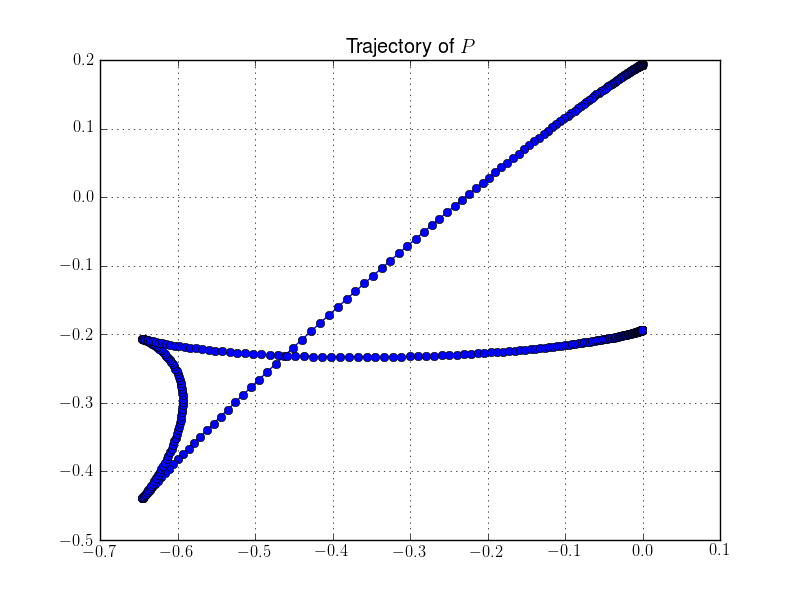
\includegraphics[width=0.5\linewidth]{./figures/tunnel_basic/phi0_trajectory_P.png}
  }
  \subfloat[][]{
    \label{fig:traject_phi0_Q}
    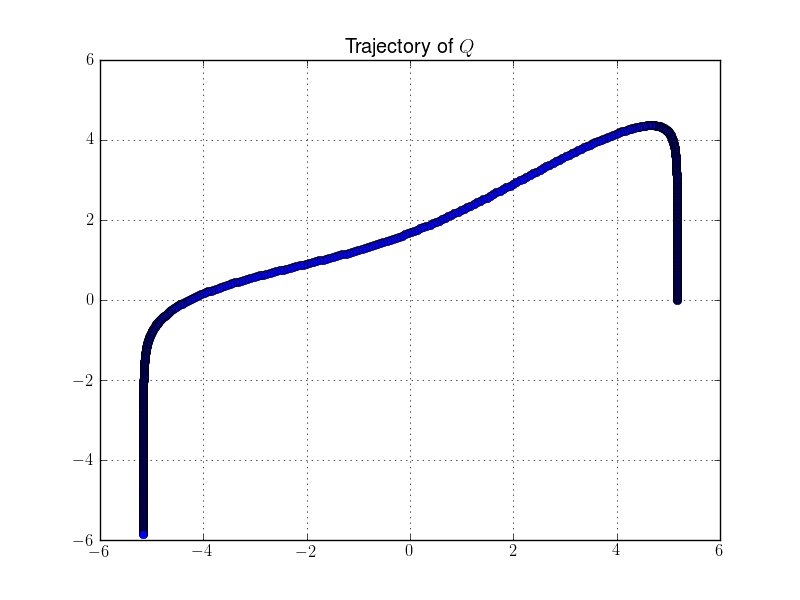
\includegraphics[width=0.5\linewidth]{./figures/tunnel_basic/phi0_trajectory_Q.png}
  } \\
  \caption[Complex trajectories for $P$ and $Q$]{
  The plot shows the trajectories of the parameters $P$ and $Q$ in the complex plane.
  The simulation parameters are shown in \ref{cfg:tunneling_phi0}.
  \label{fig:traject_phi0}
  }
\end{figure}

\begin{figure}[h!]
  \centering
  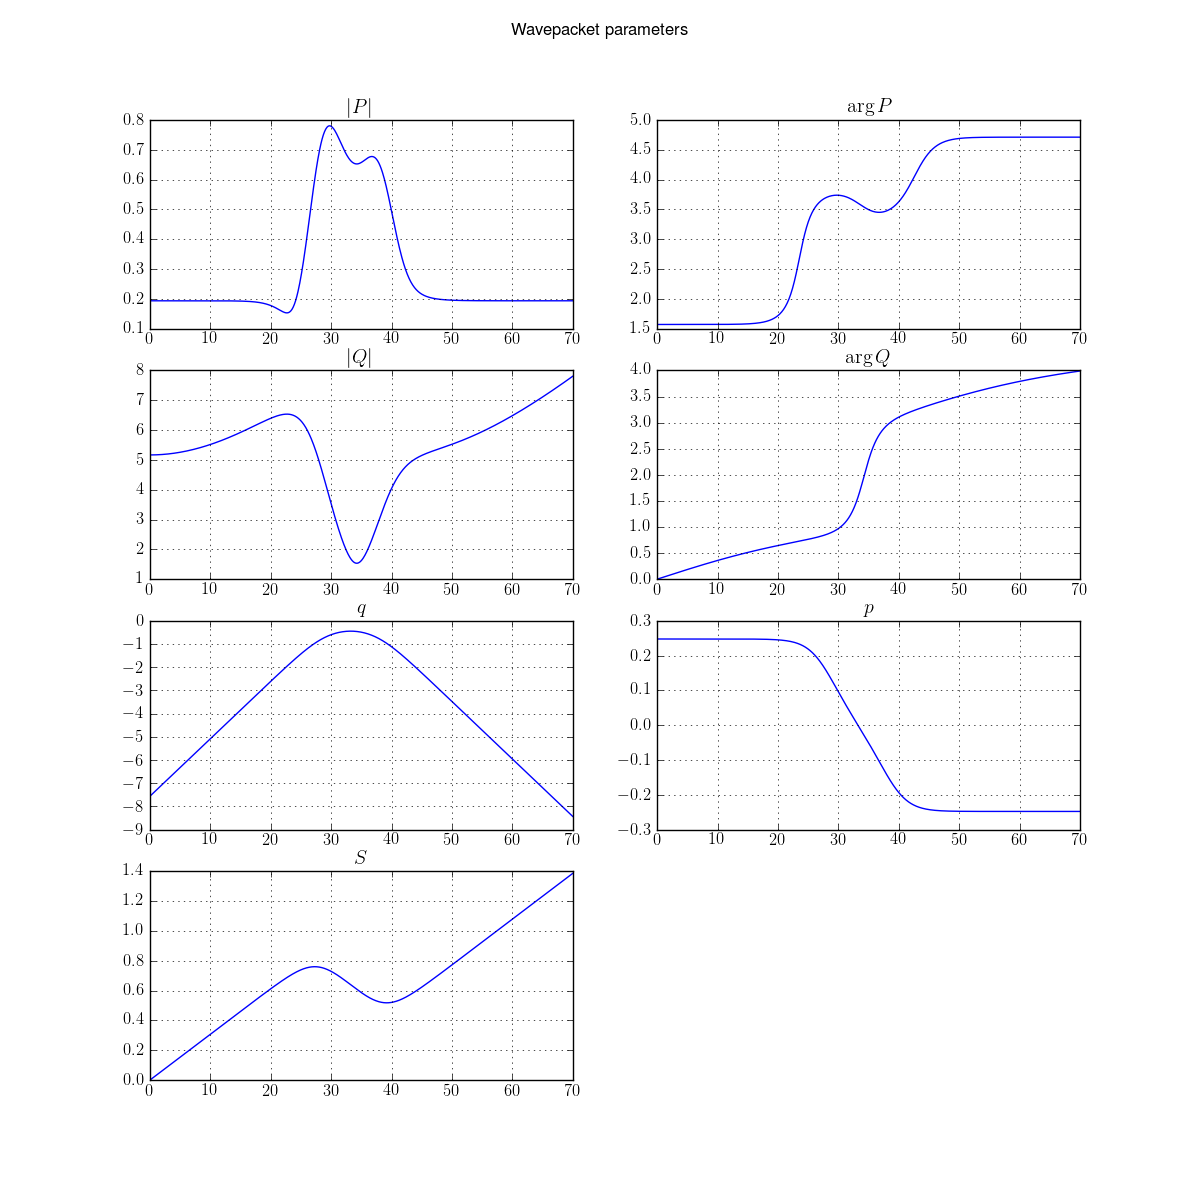
\includegraphics[width=\the\linewidth]{./figures/tunnel_basic/parameters_phi0.png}
  \caption[The parameter set $\Pi$ of the simulation with $\phi_0$]
  {The parameter set $\Pi$ of the simulation with $\phi_0$ plotted versus time.
  The simulation parameters are shown in \ref{cfg:tunneling_phi0}.}
\end{figure}

\begin{figure}[h!]
  \centering
  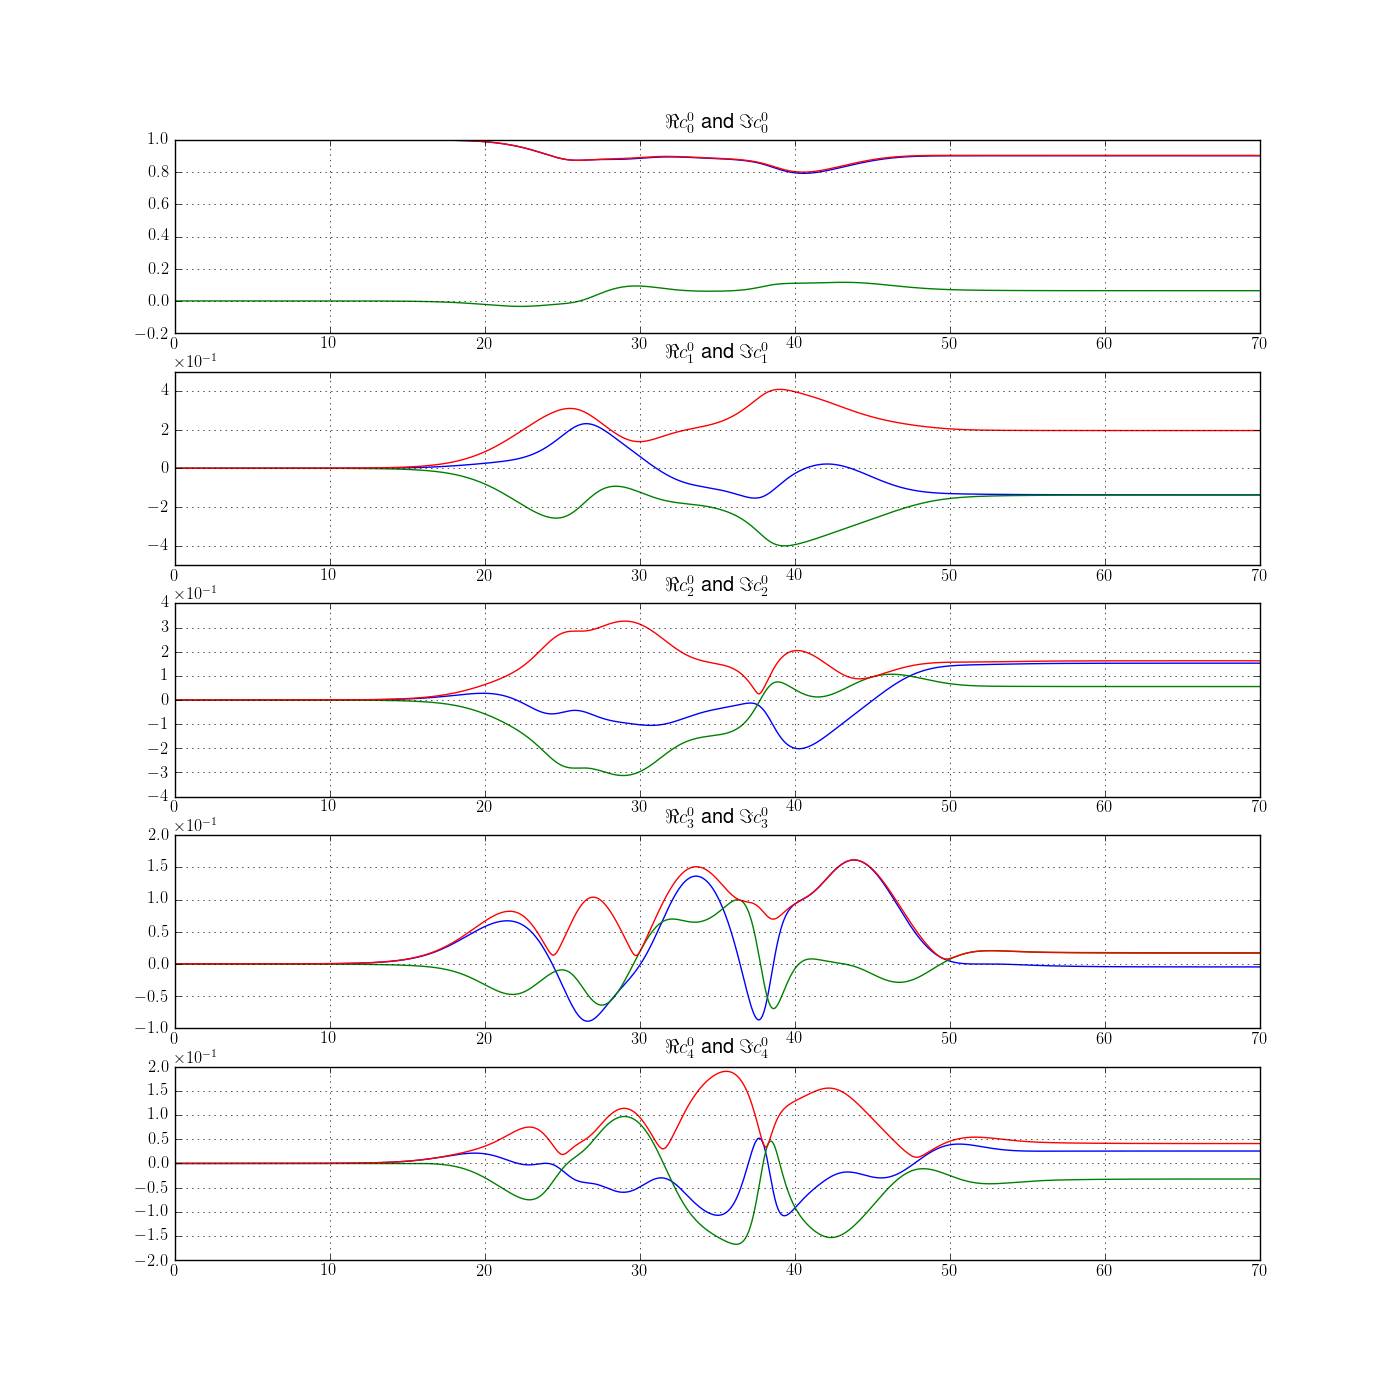
\includegraphics[width=\the\linewidth]{./figures/tunnel_basic/coefficients_first_phi0.png}
  \caption[The first few coefficients $c_i$ of the simulation with $\phi_0$]
  {The first few coefficients $c_i$ of the simulation with $\phi_0$ plotted versus time.
  The simulation parameters are shown in \ref{cfg:tunneling_phi0}.}
\end{figure}

\begin{figure}
  \centering
  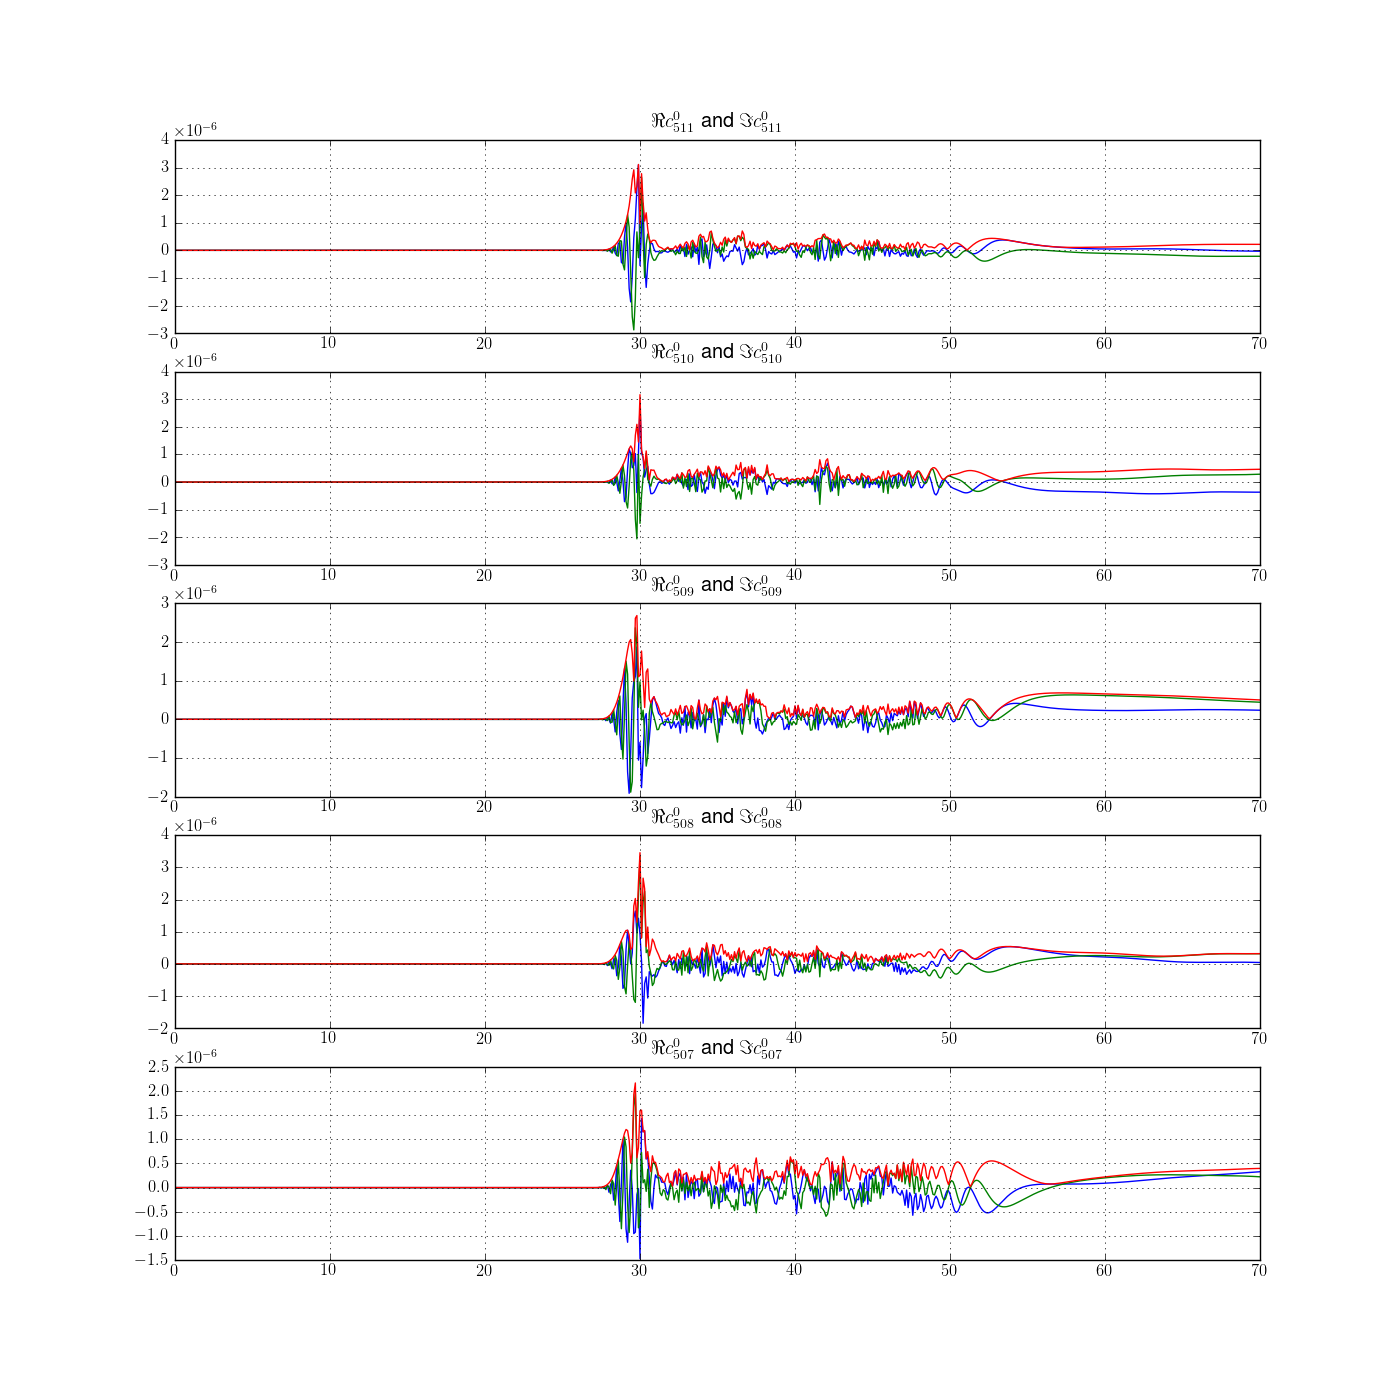
\includegraphics[width=\the\linewidth]{./figures/tunnel_basic/coefficients_last_phi0.png}
  \caption[The last few coefficients $c_i$ of the simulation with $\phi_0$]
  {The last few coefficients $c_i$ of the simulation with $\phi_0$ plotted versus time.
  We see that their values are really small and thus the loss due to the finite basis is minimal.
  The simulation parameters are shown in \ref{cfg:tunneling_phi0}.}
\end{figure}

\begin{figure}[h!]
  \centering
  \subfloat[][]{
    \label{fig:tunnel_energy_phi0}
    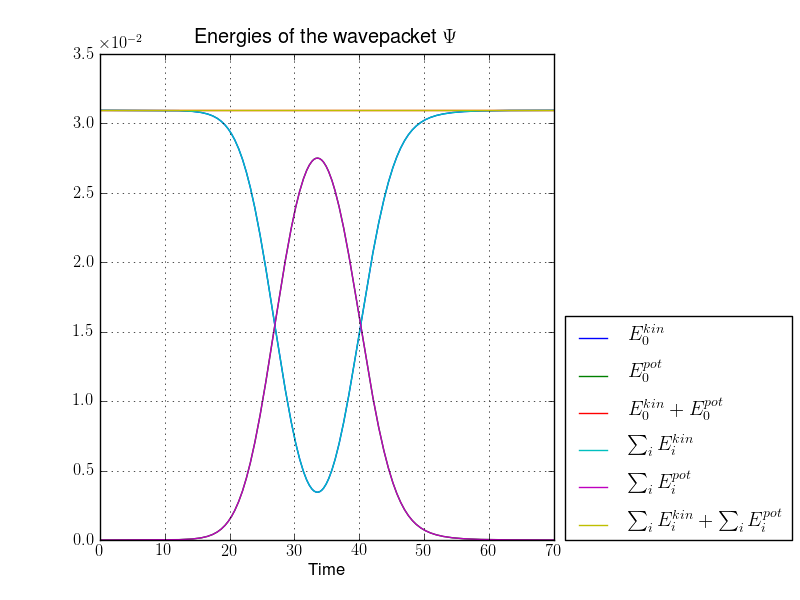
\includegraphics[width=0.5\linewidth]{./figures/tunnel_basic/energies_phi0.png}
  }
  \subfloat[][]{
    \label{fig:tunnel_energy_drift_phi0}
    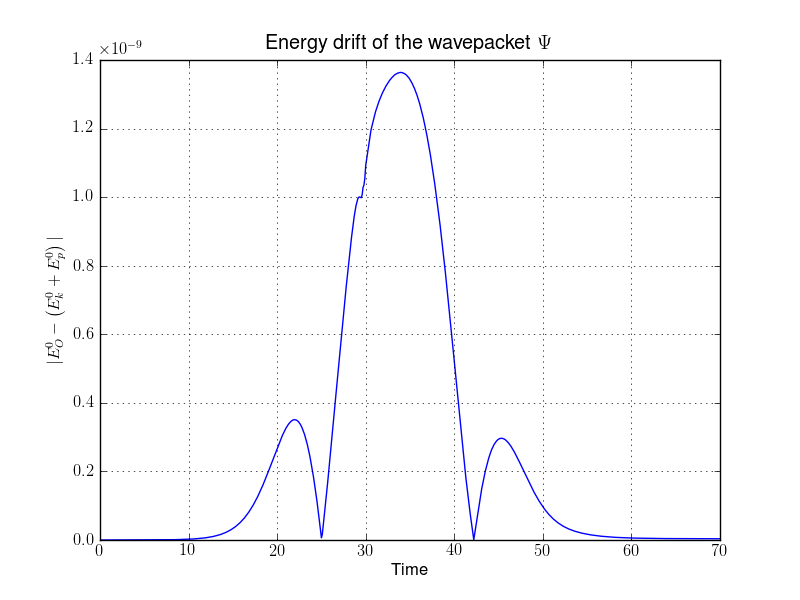
\includegraphics[width=0.5\linewidth]{./figures/tunnel_basic/energy_drift_phi0.png}
  } \\
  \subfloat[][]{
    \label{fig:tunnel_energy_phi2}
    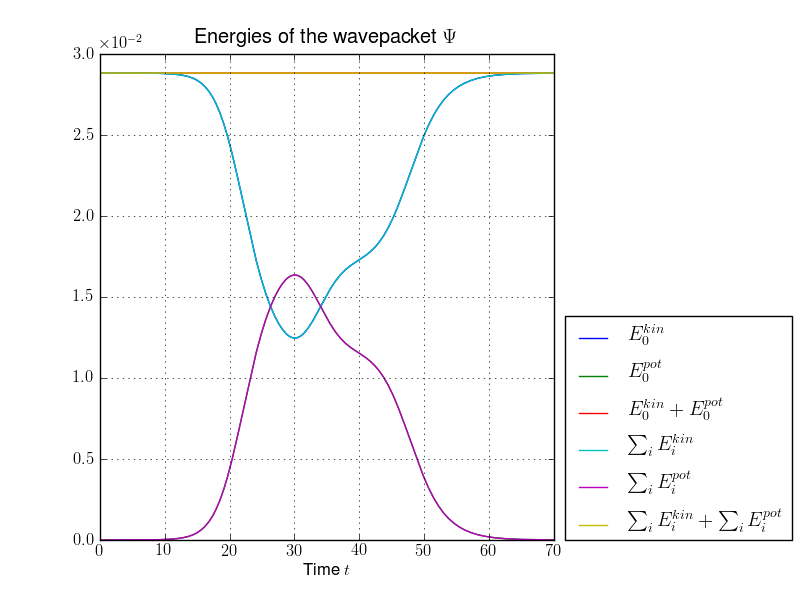
\includegraphics[width=0.5\linewidth]{./figures/tunnel_basic/energies_phi2.png}
  }
  \subfloat[][]{
    \label{fig:tunnel_energy_drift_phi2}
    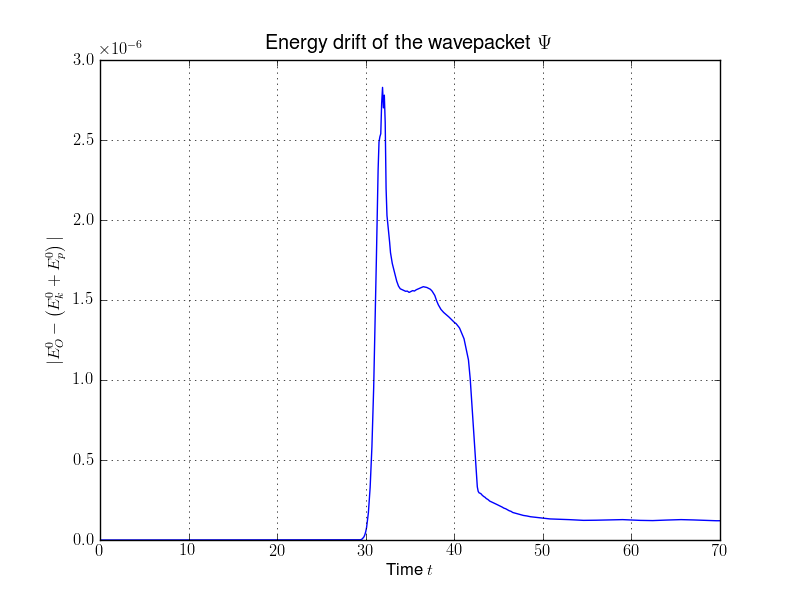
\includegraphics[width=0.5\linewidth]{./figures/tunnel_basic/energy_drift_phi2.png}
  } \\
  \subfloat[][]{
    \label{fig:tunnel_energy_phi3}
    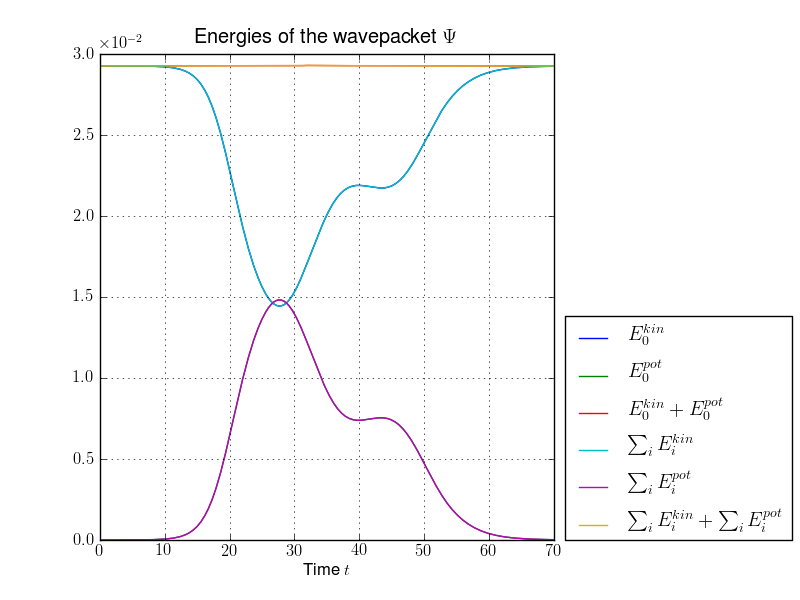
\includegraphics[width=0.5\linewidth]{./figures/tunnel_basic/energies_phi3.png}
  }
  \subfloat[][]{
    \label{fig:tunnel_energy_drift_phi3}
    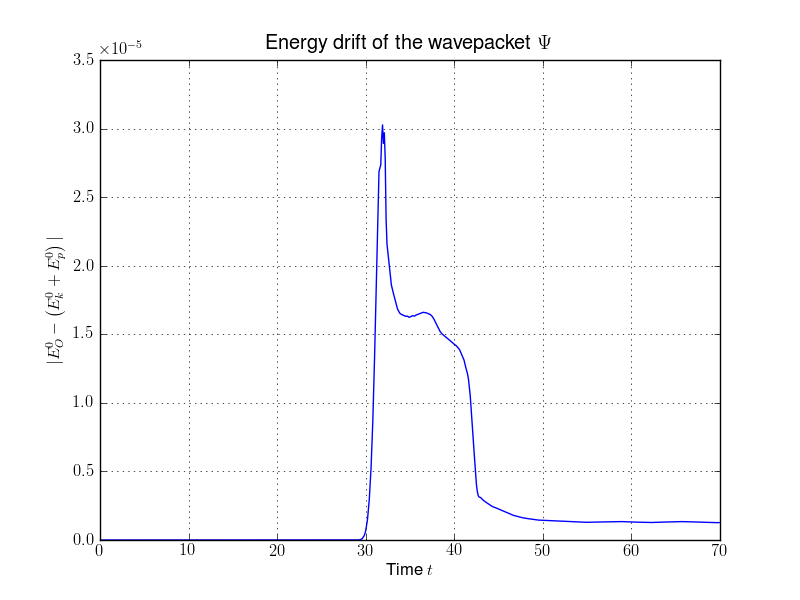
\includegraphics[width=0.5\linewidth]{./figures/tunnel_basic/energy_drift_phi3.png}
  } \\
  \caption[Energies and energy drift for some tunneling wavepackets]{
  This figure shows the energies and energy drift of several tunneling simulations.
  The simulation parameters are printed in \ref{cfg:tunneling_phi0}, \ref{cfg:tunneling_phi2} and \ref{cfg:tunneling_phi3}.
  \subref{fig:tunnel_energy_phi0} Kinetic and potential energy for a wavepacket $\phi_0$ tunneling through the Eckart barrier.
  \subref{fig:tunnel_energy_drift_phi0} Energy drift for a wavepacket $\phi_0$ tunneling through the Eckart barrier.
  \subref{fig:tunnel_energy_phi2} Kinetic and potential energy for a wavepacket $\phi_2$ tunneling through the Eckart barrier.
  \subref{fig:tunnel_energy_drift_phi2} Energy drift for a wavepacket $\phi_2$ tunneling through the Eckart barrier.
  \subref{fig:tunnel_energy_phi3} Kinetic and potential energy for a wavepacket $\phi_3$ tunneling through the Eckart barrier.
  \subref{fig:tunnel_energy_drift_phi3} Energy drift for a wavepacket $\phi_3$ tunneling through the Eckart barrier.
  \label{fig:tunnel_energies}
  }
\end{figure}

\begin{figure}[h!]
  \centering
  \subfloat[][]{
    \label{fig:tunnel_norm_drift_phi0}
    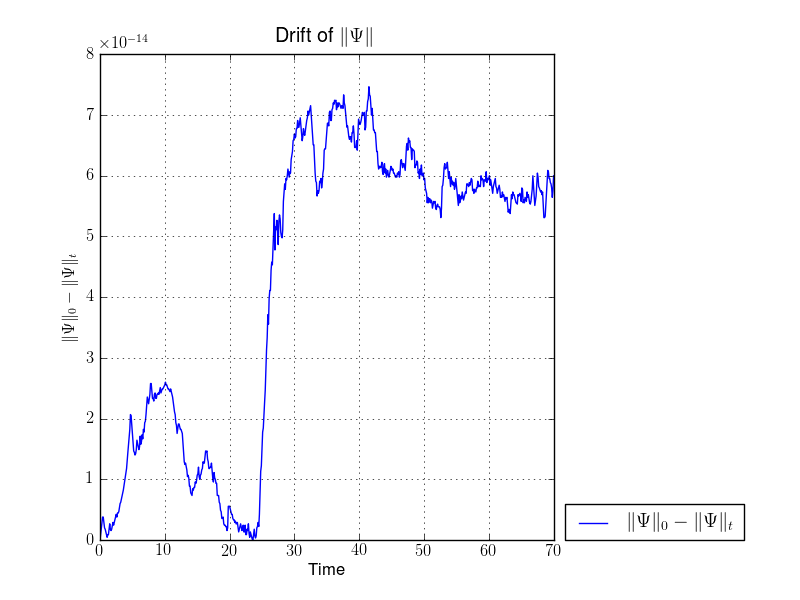
\includegraphics[width=0.5\linewidth]{./figures/tunnel_basic/norms_drift_phi0.png}
  }
  \subfloat[][]{
    \label{fig:tunnel_norm_drift_phi2}
    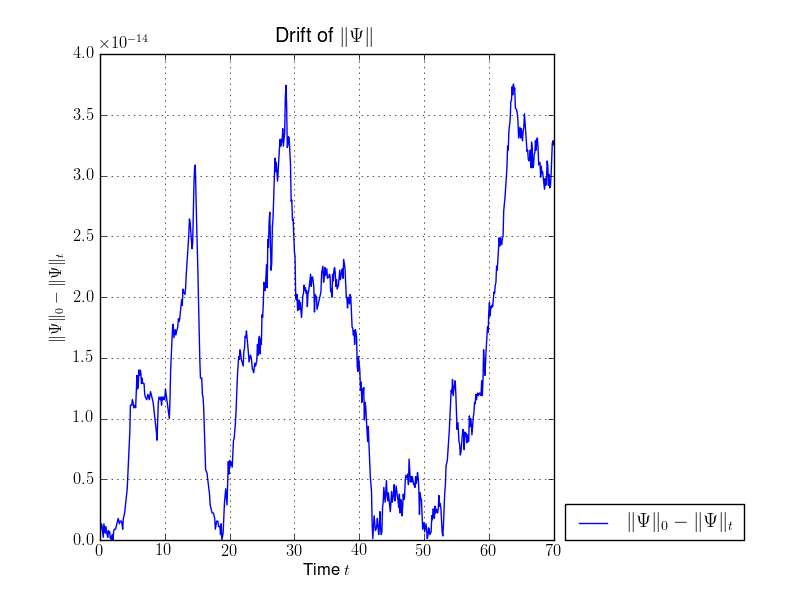
\includegraphics[width=0.5\linewidth]{./figures/tunnel_basic/norms_drift_phi2.png}
  } \\
  \subfloat[][]{
    \label{fig:tunnel_norm_drift_phi3}
    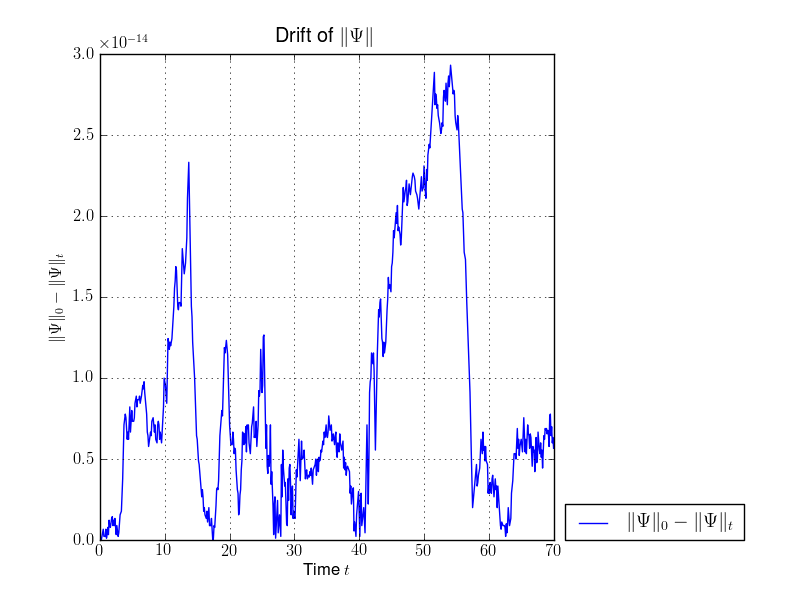
\includegraphics[width=0.5\linewidth]{./figures/tunnel_basic/norms_drift_phi3.png}
  }
  \caption[Norm drift for some tunneling wavepackets]{
  This figure shows the drift of the norm for several tunneling simulations. We have very good
  norm conservation. The reason for this is that we used a huge basis with $K=512$.
  The simulation parameters are printed in \ref{cfg:tunneling_phi0}, \ref{cfg:tunneling_phi2} and \ref{cfg:tunneling_phi3}.
  \subref{fig:tunnel_norm_drift_phi0} Norm drift for a wavepacket $\phi_0$ tunneling through the Eckart barrier.
  \subref{fig:tunnel_norm_drift_phi2} Norm drift for a wavepacket $\phi_2$ tunneling through the Eckart barrier.
  \subref{fig:tunnel_norm_drift_phi3} Norm drift for a wavepacket $\phi_3$ tunneling through the Eckart barrier.
  \label{fig:tunnel_norms}
  }
\end{figure}


\FloatBarrier
\section{Spawning using the lumping method}

Now we try aposteriori spawning based on the simulation from the last section.
In the first examples we use the lumping method which works quite well for large
enough times. The spawned packet has the shape of a Gaussian and we set $k=0$ for
lumping. The initial values of $\Ket{\Psi}$ are taken to be $\phi_0$, $\phi_2$
and $\phi_3$. We try different values for the parameter $K_0$ and compare the
estimated parameter sets $\tilde{\Pi}$.


\begin{figure}[h!]
  \centering
  \subfloat[][]{
    \label{fig:spawn_eckart_apost_phi0_K050_norms}
    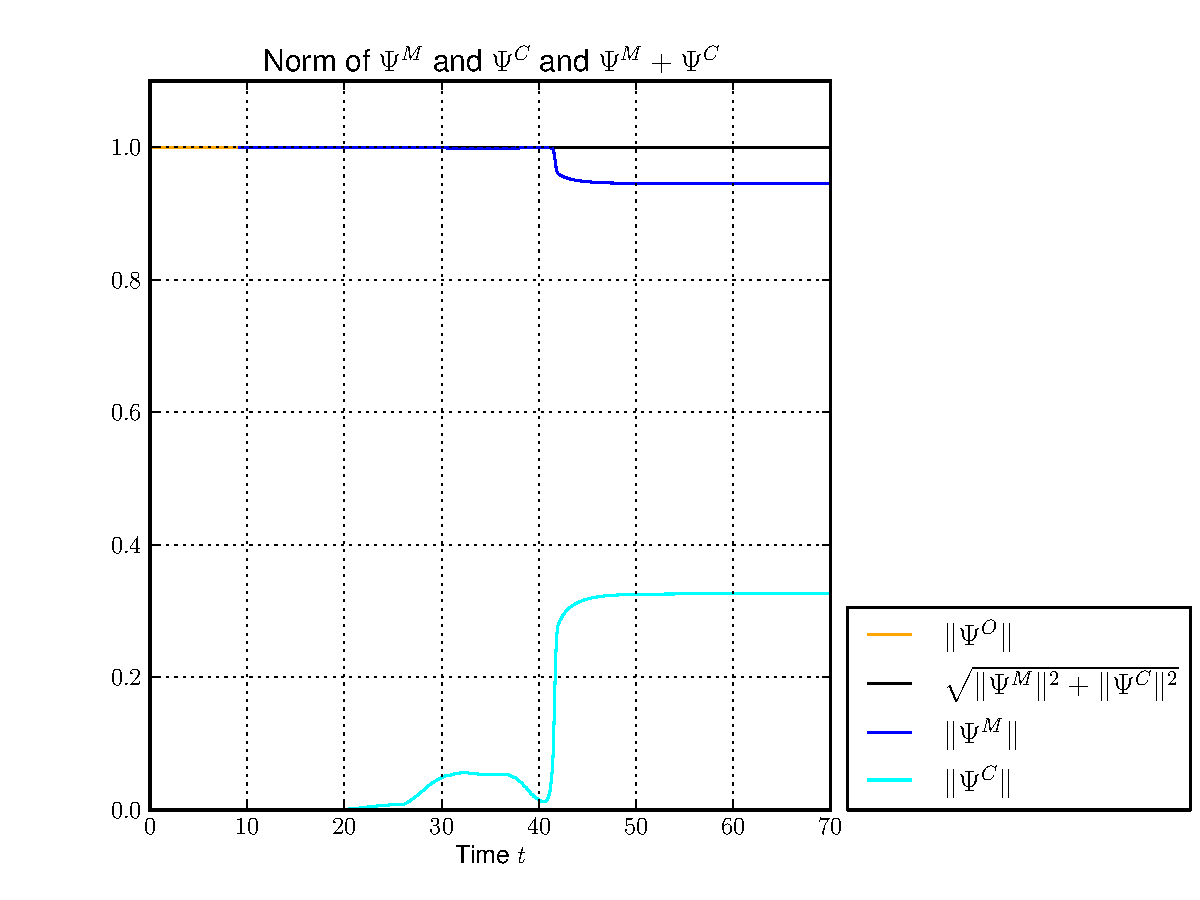
\includegraphics[width=0.5\linewidth]{./figures/eckart_spawn_apost_phi0_K50/norms_compare_sumall_group0.pdf}
  }
  \subfloat[][]{
    \label{fig:spawn_eckart_apost_phi0_K050_norms_drift}
    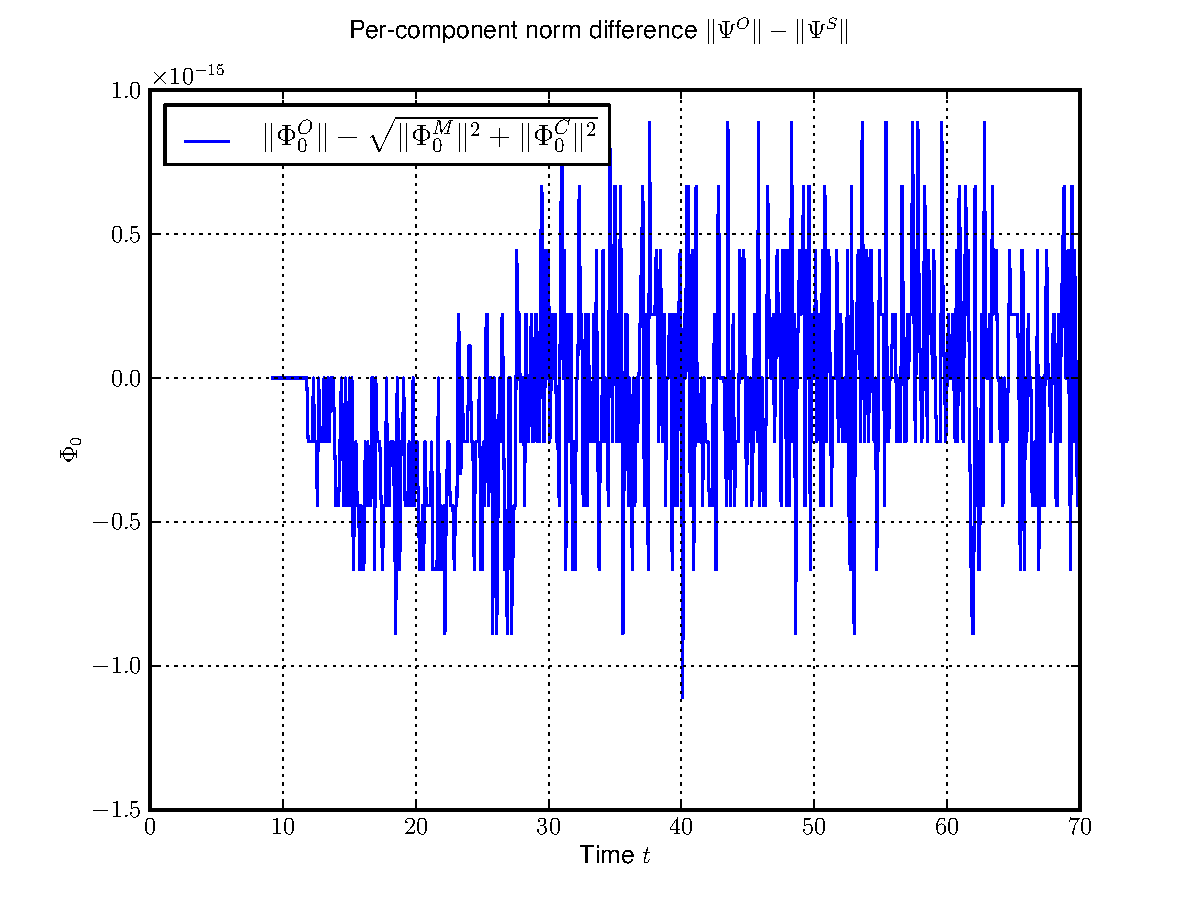
\includegraphics[width=0.5\linewidth]{./figures/eckart_spawn_apost_phi0_K50/norms_compare_components_diff_group0.pdf}
  } \\
  \subfloat[][]{
    \label{fig:spawn_eckart_apost_phi0_K075_norms}
    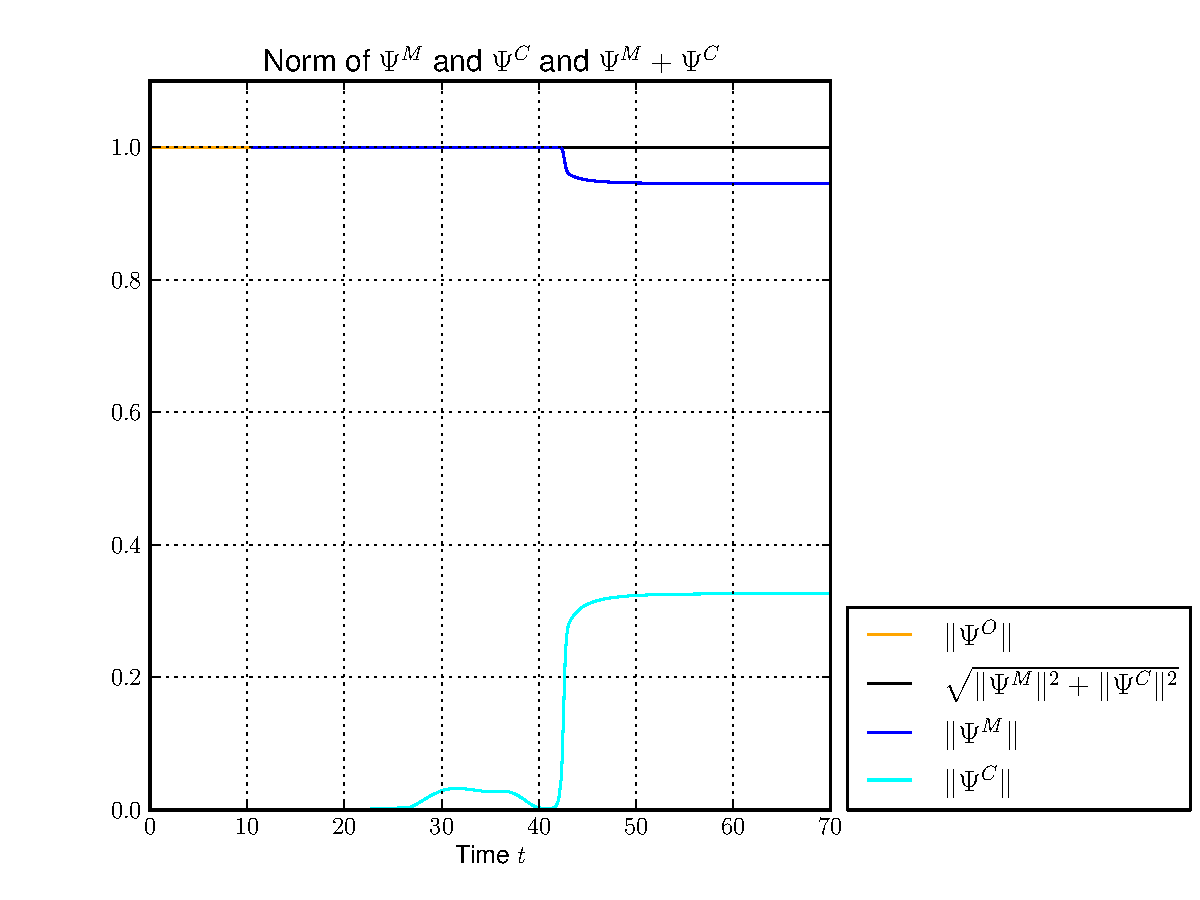
\includegraphics[width=0.5\linewidth]{./figures/eckart_spawn_apost_phi0_K75/norms_compare_sumall_group0.pdf}
  }
  \subfloat[][]{
    \label{fig:spawn_eckart_apost_phi0_K075_norms_drift}
    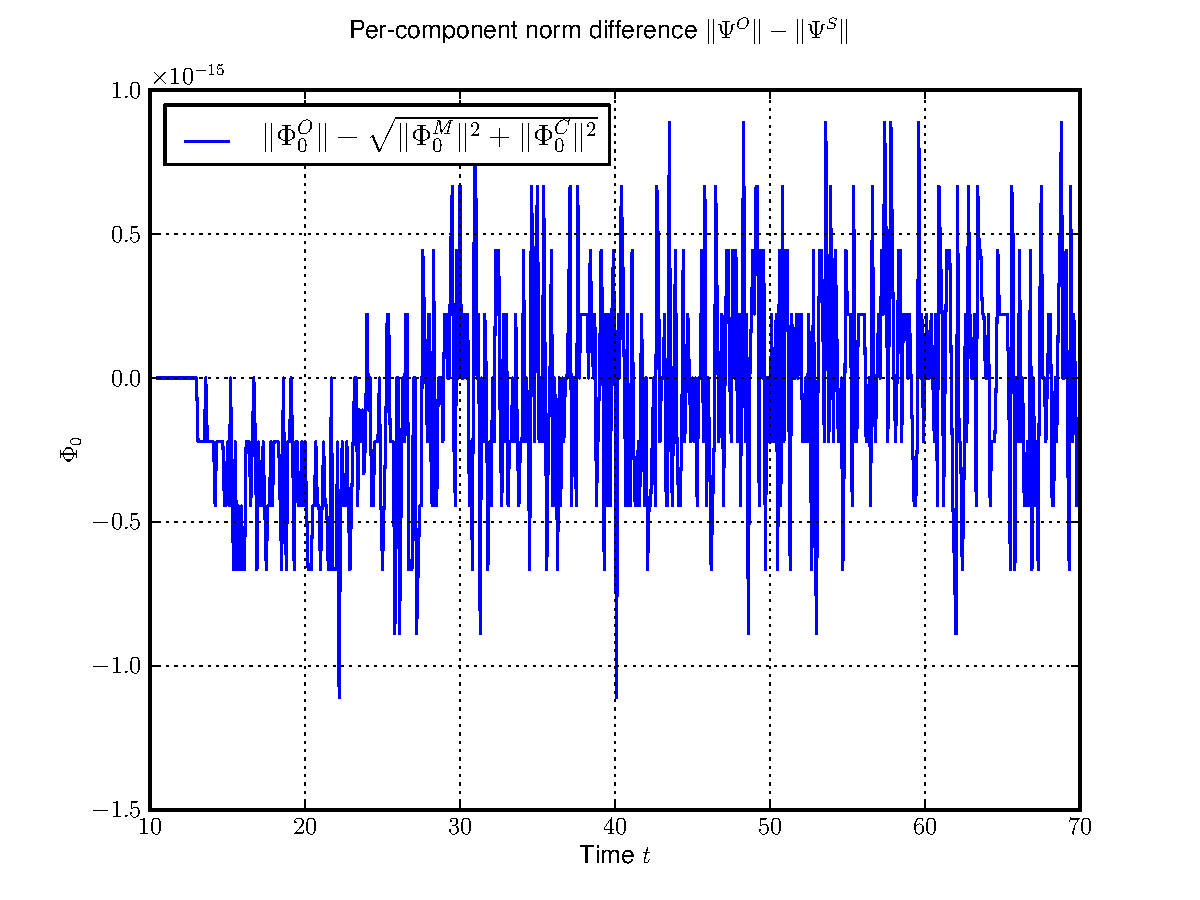
\includegraphics[width=0.5\linewidth]{./figures/eckart_spawn_apost_phi0_K75/norms_compare_components_diff_group0.pdf}
  } \\
  \subfloat[][]{
    \label{fig:spawn_eckart_apost_phi0_K0100_norms}
    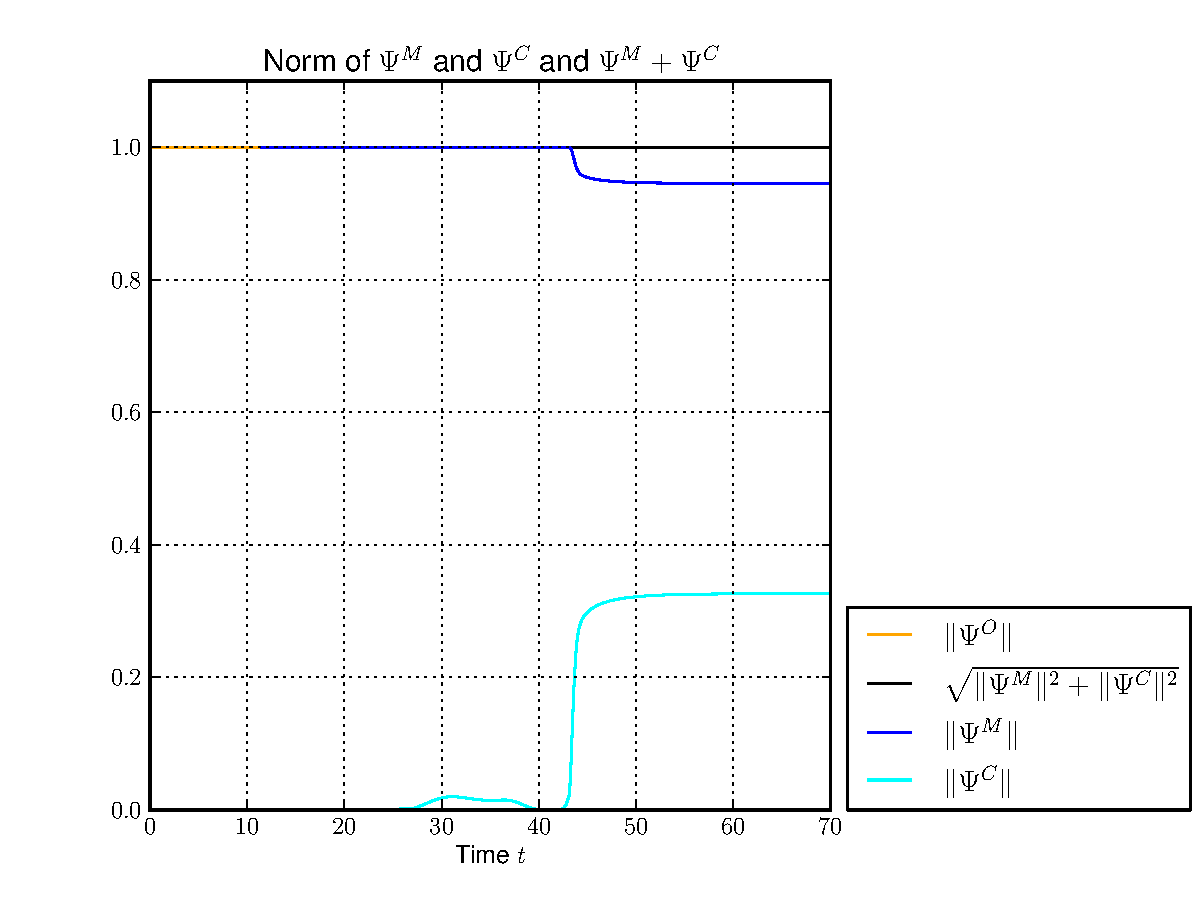
\includegraphics[width=0.5\linewidth]{./figures/eckart_spawn_apost_phi0_K100/norms_compare_sumall_group0.pdf}
  }
  \subfloat[][]{
    \label{fig:spawn_eckart_apost_phi0_K0100_norms_drift}
    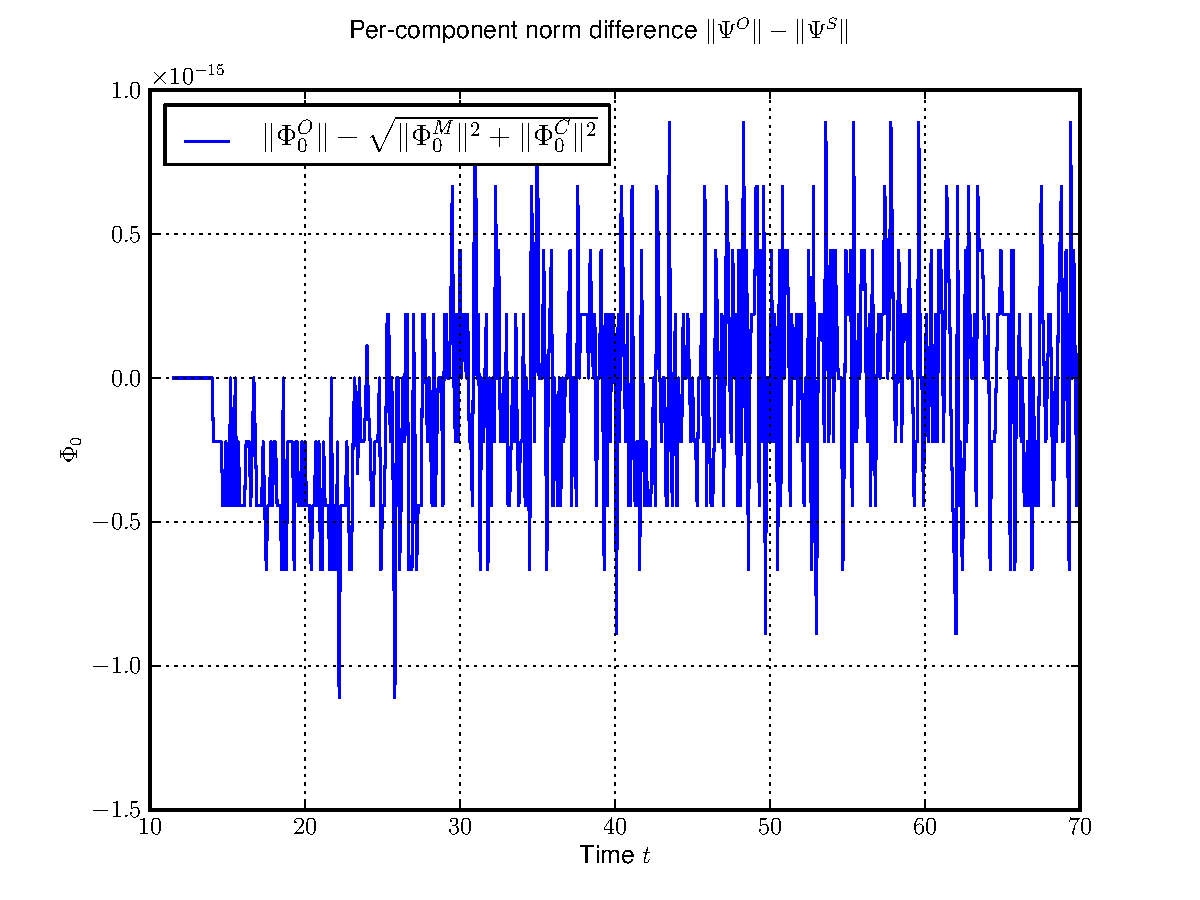
\includegraphics[width=0.5\linewidth]{./figures/eckart_spawn_apost_phi0_K100/norms_compare_components_diff_group0.pdf}
  } \\
  \caption[Norms and norm drift for an aposteriori spawning simulation with lumping]{
  Norms and norm drift for an aposteriori spawning simulation based on the tunneling
  simulation of $\phi_0$. We see perfect norm conservation which has to be expected
  because of the lumping process which is lossless.
  \subref{fig:spawn_eckart_apost_phi0_K050_norms} $\Psi = \phi_0$ and $K_0=50$
  \subref{fig:spawn_eckart_apost_phi0_K050_norms_drift} $\Psi = \phi_0$ and $K_0=50$
  \subref{fig:spawn_eckart_apost_phi0_K075_norms} $\Psi = \phi_0$ and $K_0=75$
  \subref{fig:spawn_eckart_apost_phi0_K075_norms_drift} $\Psi = \phi_0$ and $K_0=75$
  \subref{fig:spawn_eckart_apost_phi0_K0100_norms} $\Psi = \phi_0$ and $K_0=100$
  \subref{fig:spawn_eckart_apost_phi0_K0100_norms_drift} $\Psi = \phi_0$ and $K_0=100$
  \label{fig:spawn_eckart_apost_phi0_norms}
  }
\end{figure}


\begin{figure}[h!]
  \centering
  \subfloat[][]{
    \label{fig:spawn_eckart_apost_phi2_K050_norms}
    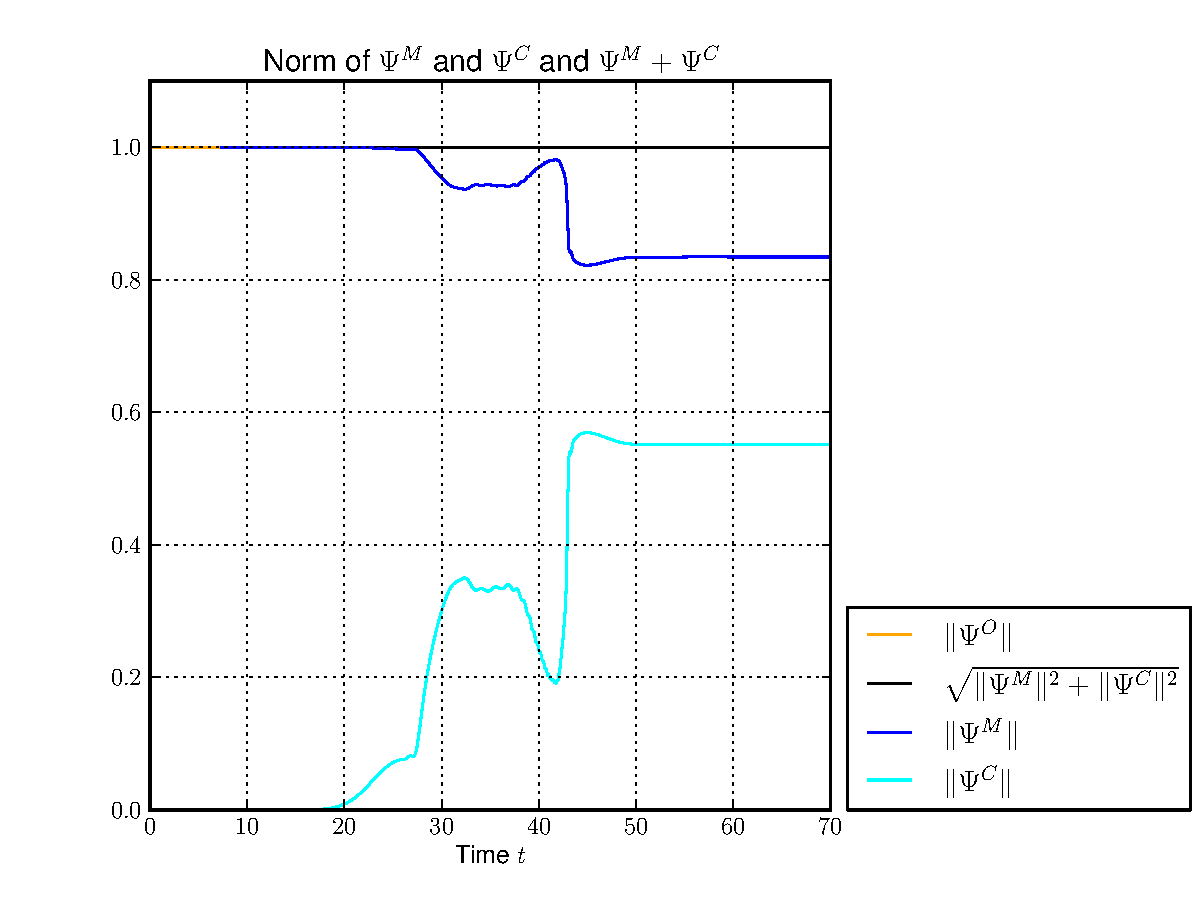
\includegraphics[width=0.5\linewidth]{./figures/eckart_spawn_apost_phi2_K50/norms_compare_sumall_group0.pdf}
  }
  \subfloat[][]{
    \label{fig:spawn_eckart_apost_phi2_K050_norms_drift}
    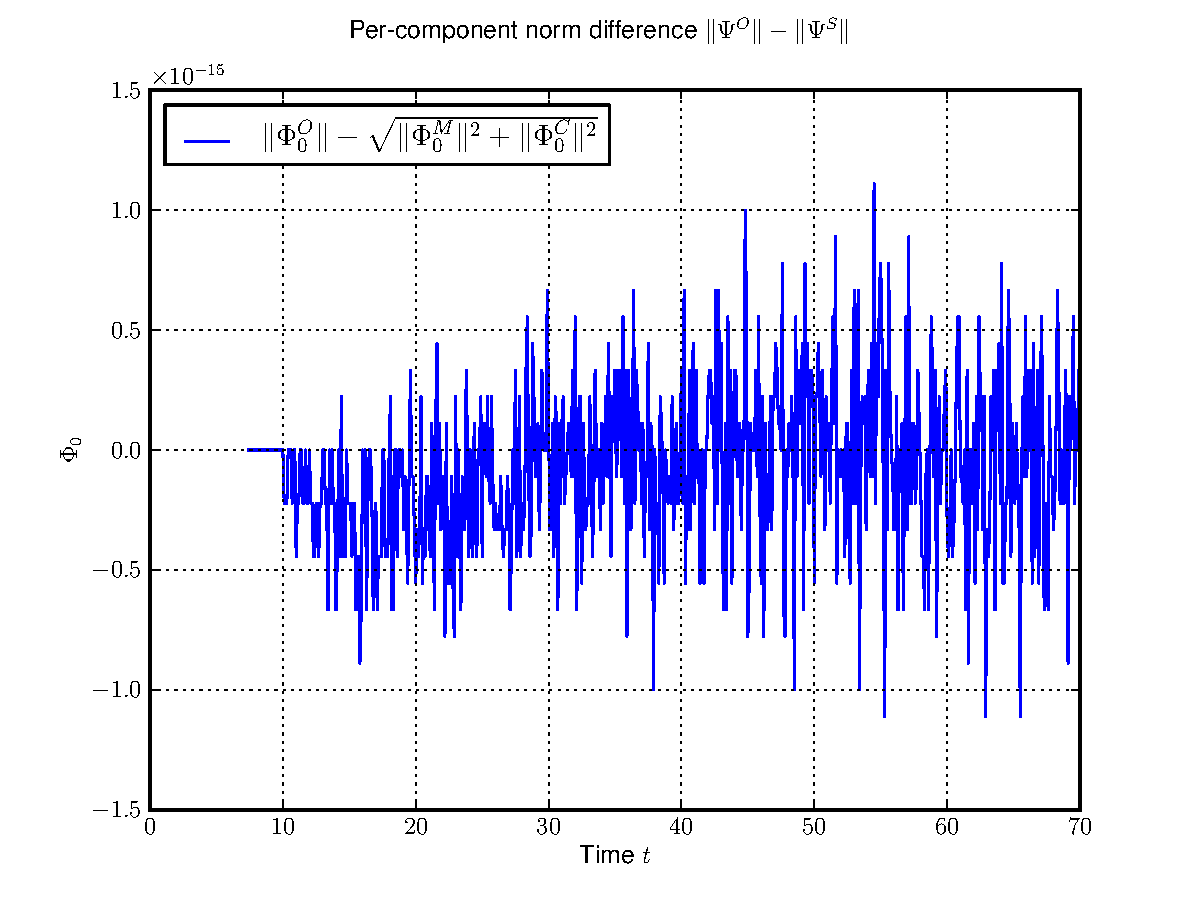
\includegraphics[width=0.5\linewidth]{./figures/eckart_spawn_apost_phi2_K50/norms_compare_components_diff_group0.pdf}
  } \\
  \subfloat[][]{
    \label{fig:spawn_eckart_apost_phi2_K075_norms}
    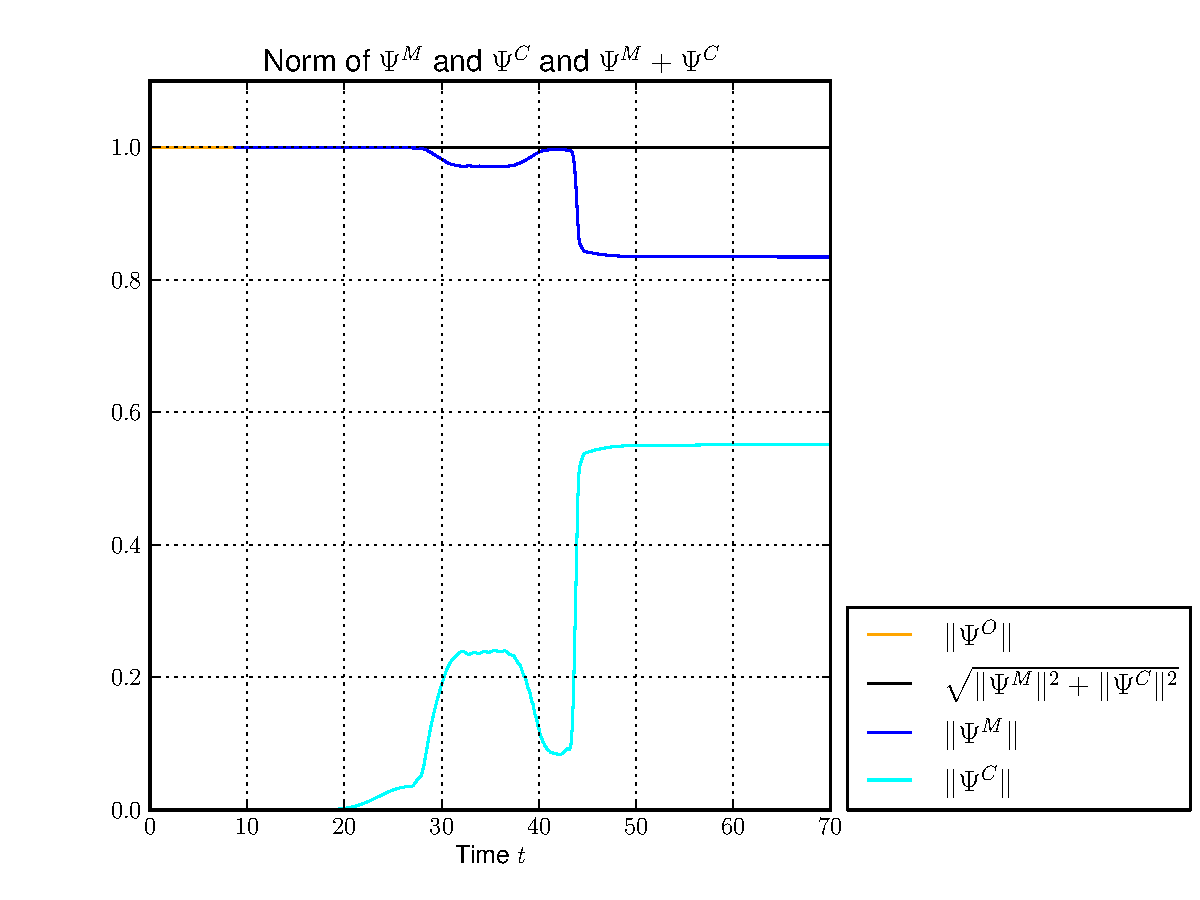
\includegraphics[width=0.5\linewidth]{./figures/eckart_spawn_apost_phi2_K75/norms_compare_sumall_group0.pdf}
  }
  \subfloat[][]{
    \label{fig:spawn_eckart_apost_phi2_K075_norms_drift}
    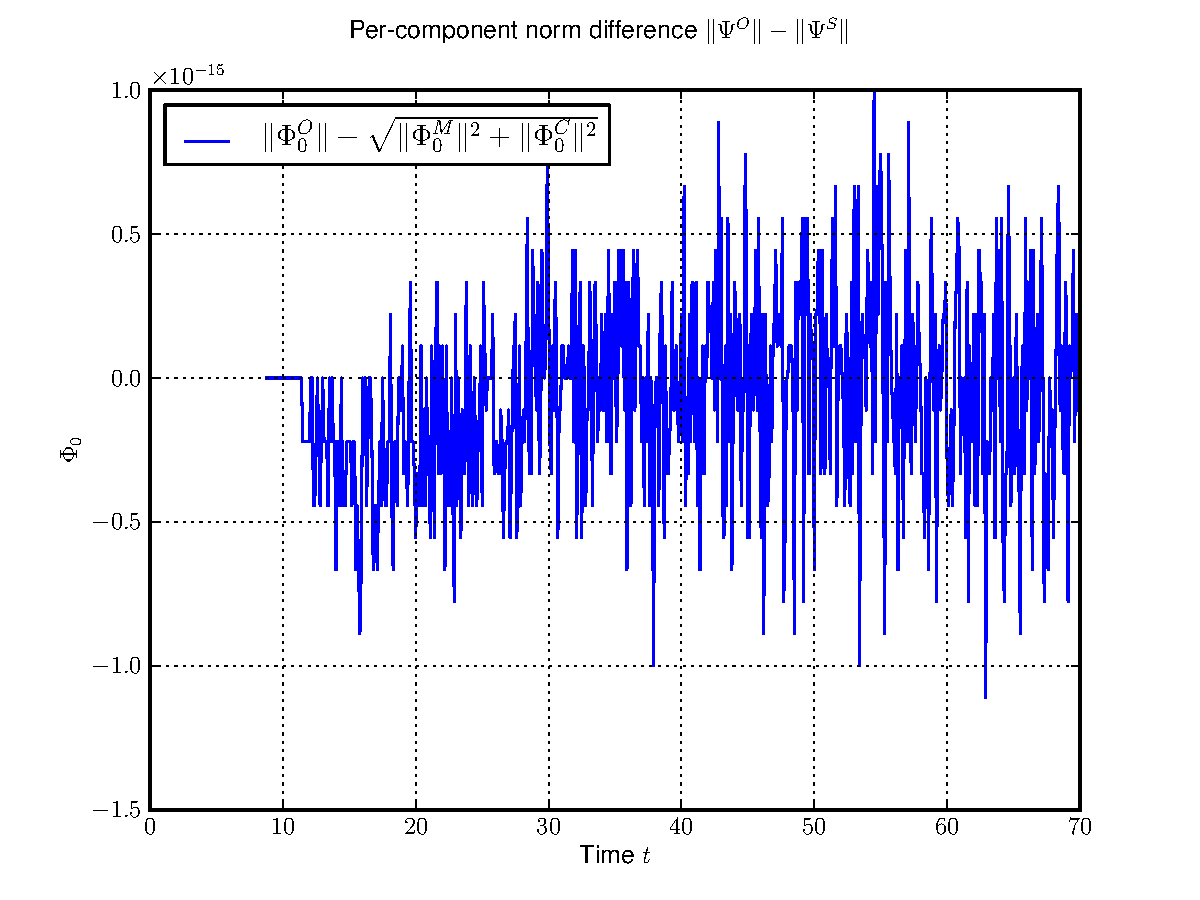
\includegraphics[width=0.5\linewidth]{./figures/eckart_spawn_apost_phi2_K75/norms_compare_components_diff_group0.pdf}
  } \\
  \subfloat[][]{
    \label{fig:spawn_eckart_apost_phi2_K0100_norms}
    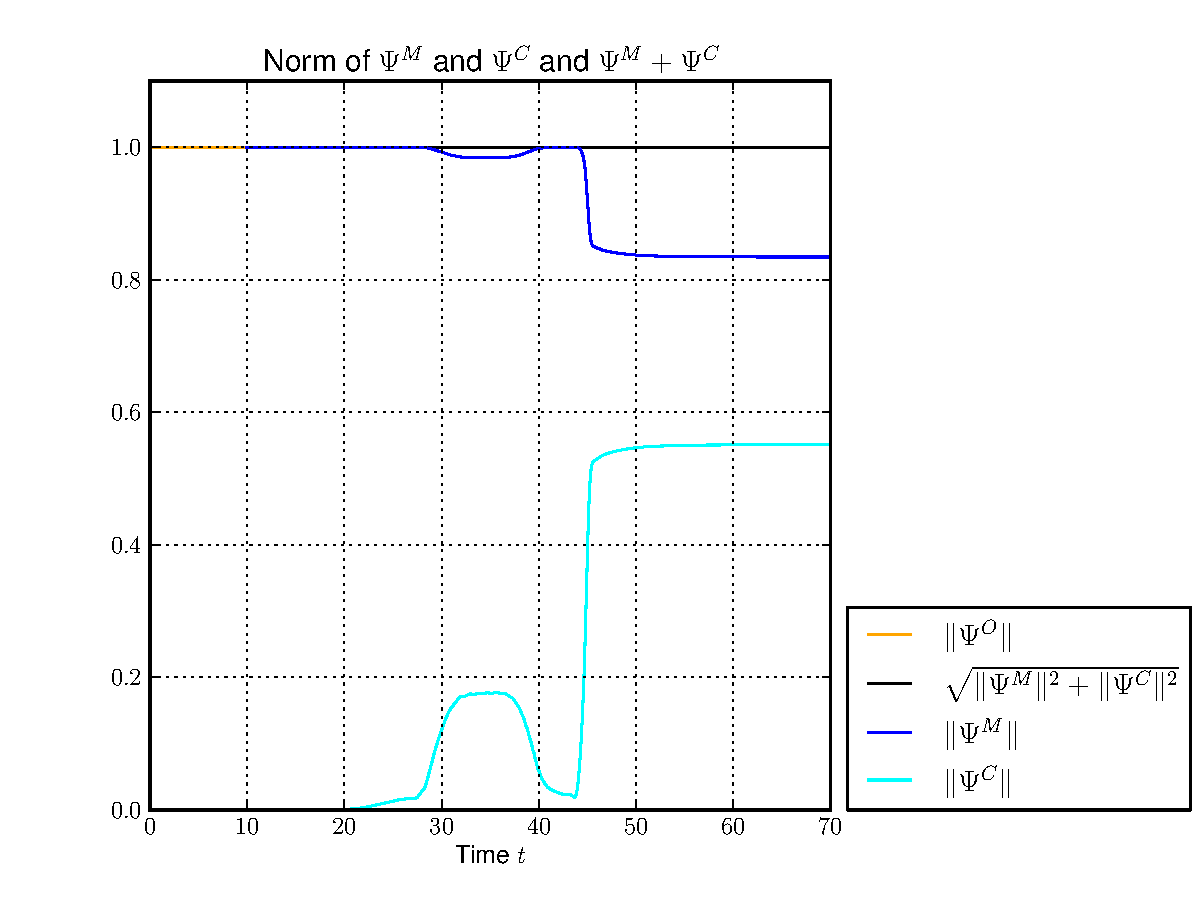
\includegraphics[width=0.5\linewidth]{./figures/eckart_spawn_apost_phi2_K100/norms_compare_sumall_group0.pdf}
  }
  \subfloat[][]{
    \label{fig:spawn_eckart_apost_phi2_K0100_norms_drift}
    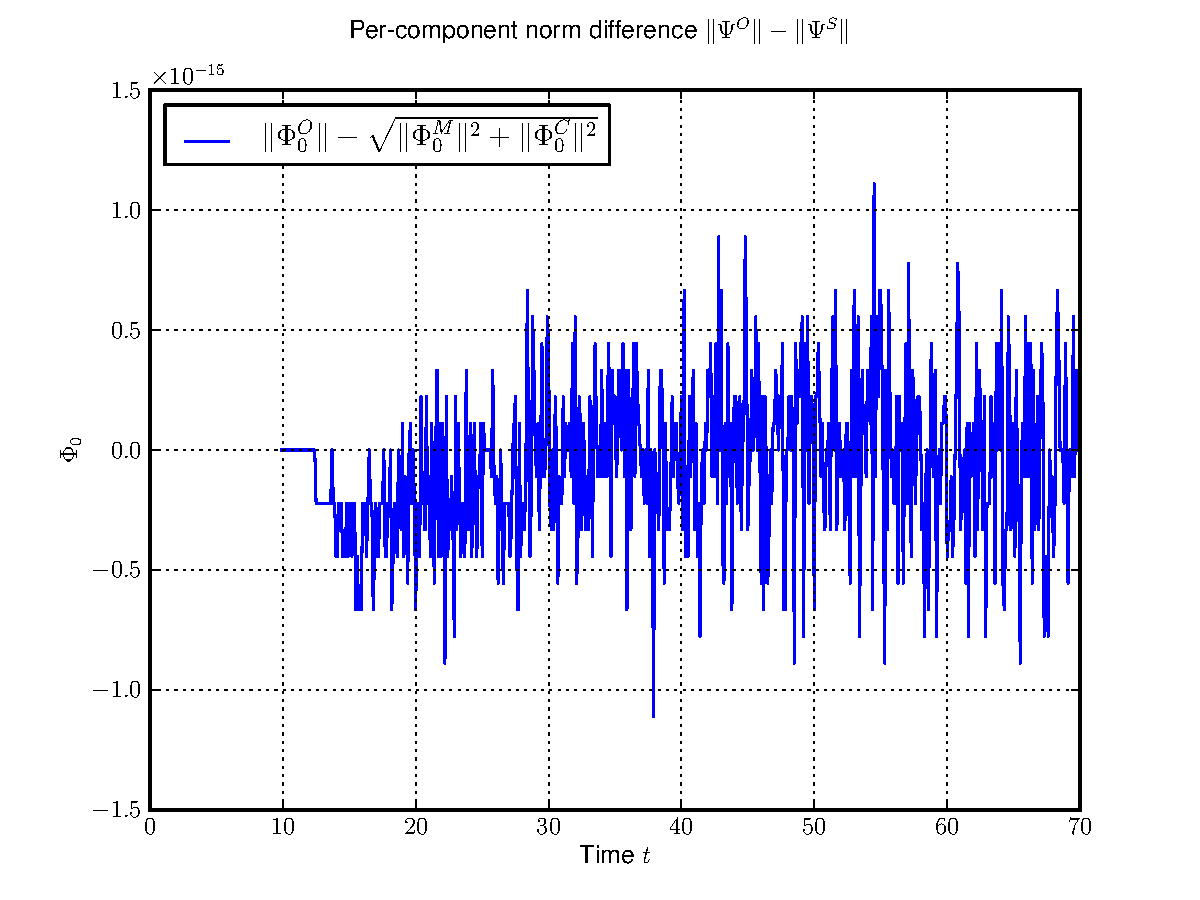
\includegraphics[width=0.5\linewidth]{./figures/eckart_spawn_apost_phi2_K100/norms_compare_components_diff_group0.pdf}
  } \\
  \caption[Norms and norm drift for an aposteriori spawning simulation with lumping]{
  Norms and norm drift for an aposteriori spawning simulation based on the tunneling
  simulation of $\phi_2$. We see perfect norm conservation which has to be expected
  because of the lumping process which is lossless.
  \subref{fig:spawn_eckart_apost_phi2_K050_norms} $\Psi = \phi_2$ and $K_0=50$
  \subref{fig:spawn_eckart_apost_phi2_K050_norms_drift} $\Psi = \phi_2$ and $K_0=50$
  \subref{fig:spawn_eckart_apost_phi2_K075_norms} $\Psi = \phi_2$ and $K_0=75$
  \subref{fig:spawn_eckart_apost_phi2_K075_norms_drift} $\Psi = \phi_2$ and $K_0=75$
  \subref{fig:spawn_eckart_apost_phi2_K0100_norms} $\Psi = \phi_2$ and $K_0=100$
  \subref{fig:spawn_eckart_apost_phi2_K0100_norms_drift} $\Psi = \phi_2$ and $K_0=100$
  \label{fig:spawn_eckart_apost_phi2_norms}
  }
\end{figure}


\begin{figure}[h!]
  \centering
  \subfloat[][]{
    \label{fig:spawn_eckart_apost_phi3_K050_norms}
    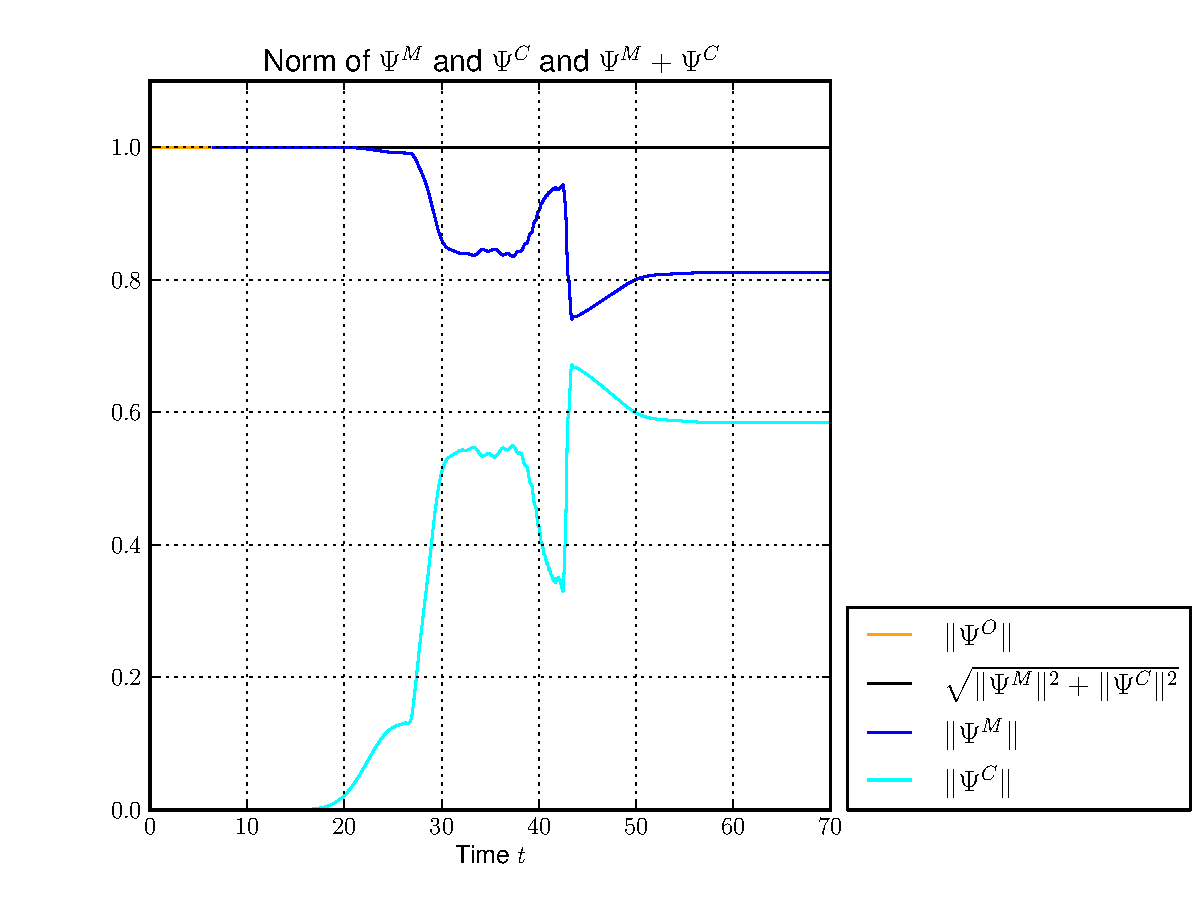
\includegraphics[width=0.5\linewidth]{./figures/eckart_spawn_apost_phi3_K50/norms_compare_sumall_group0.pdf}
  }
  \subfloat[][]{
    \label{fig:spawn_eckart_apost_phi3_K050_norms_drift}
    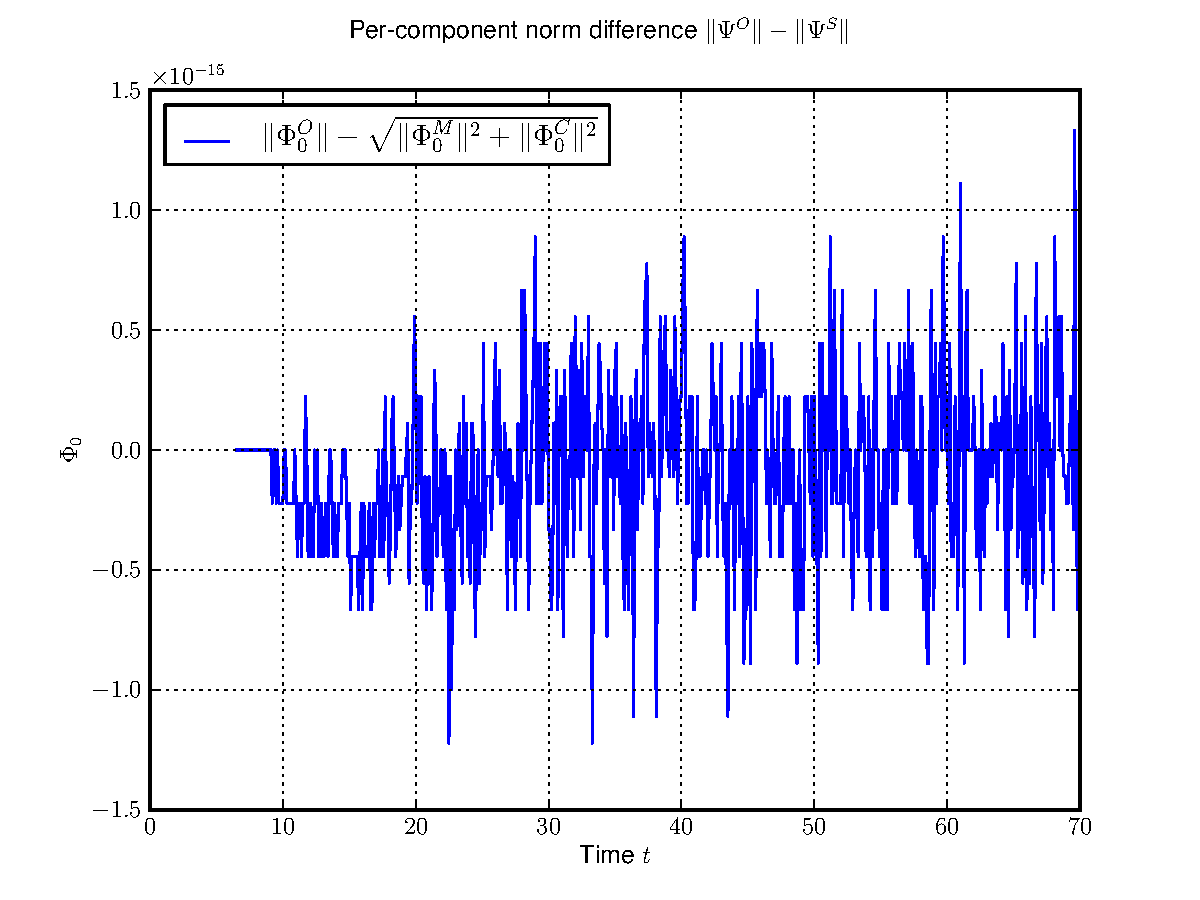
\includegraphics[width=0.5\linewidth]{./figures/eckart_spawn_apost_phi3_K50/norms_compare_components_diff_group0.pdf}
  } \\
  \subfloat[][]{
    \label{fig:spawn_eckart_apost_phi3_K075_norms}
    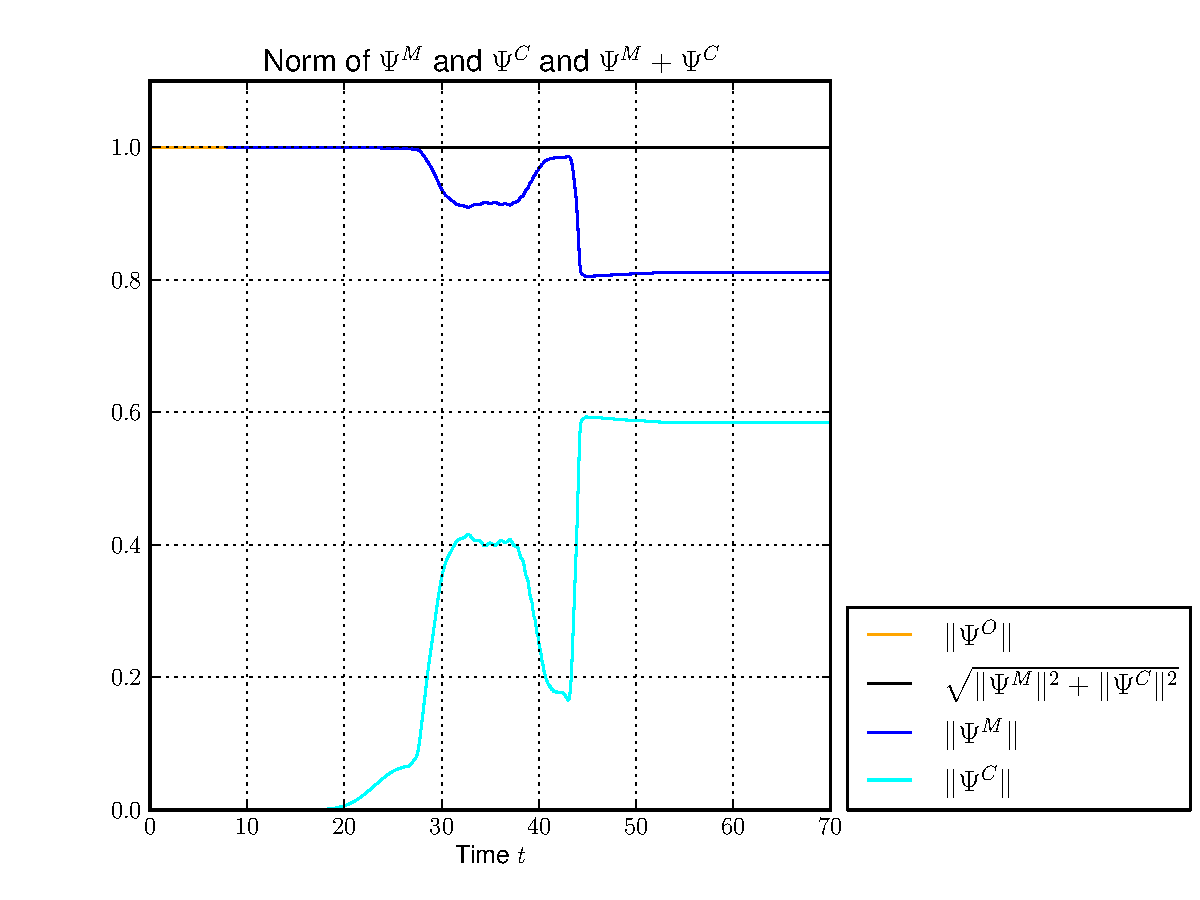
\includegraphics[width=0.5\linewidth]{./figures/eckart_spawn_apost_phi3_K75/norms_compare_sumall_group0.pdf}
  }
  \subfloat[][]{
    \label{fig:spawn_eckart_apost_phi3_K075_norms_drift}
    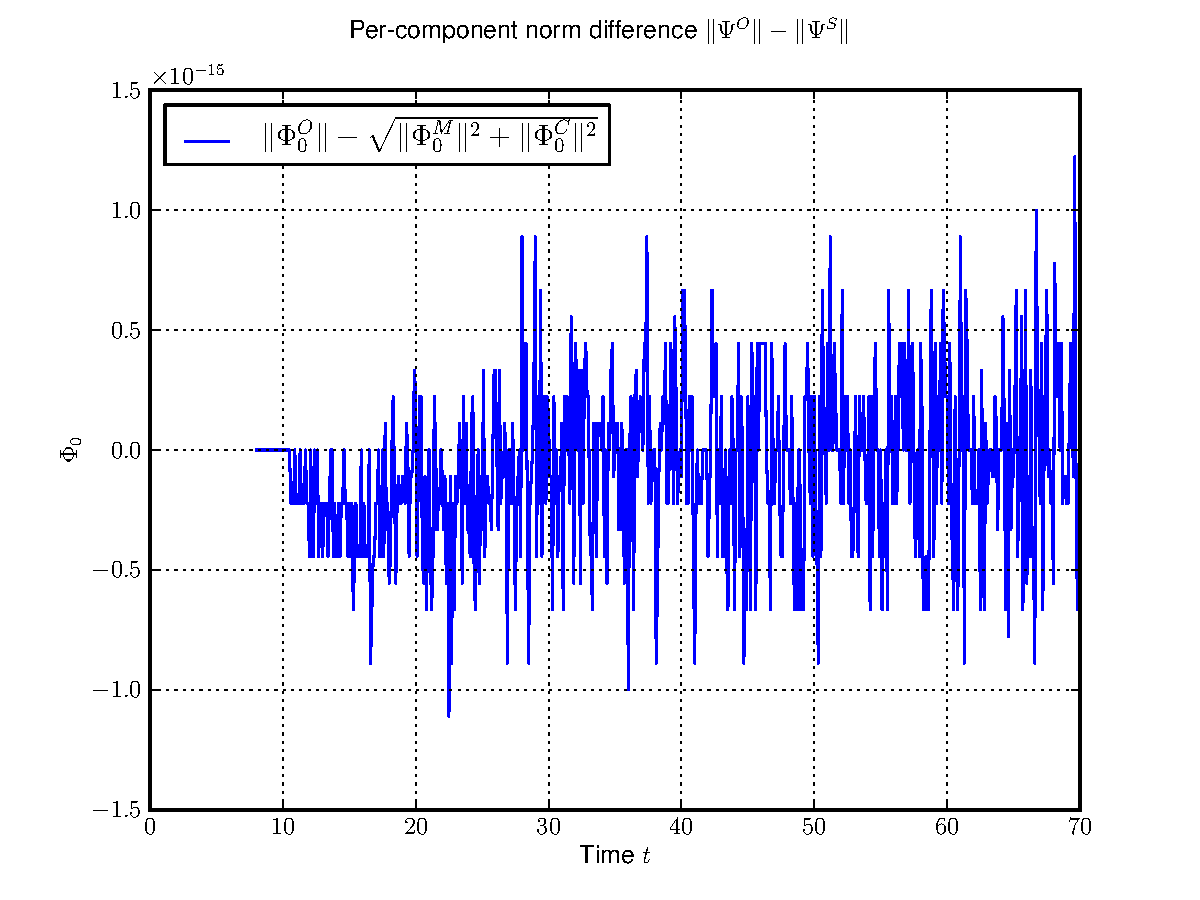
\includegraphics[width=0.5\linewidth]{./figures/eckart_spawn_apost_phi3_K75/norms_compare_components_diff_group0.pdf}
  } \\
  \subfloat[][]{
    \label{fig:spawn_eckart_apost_phi3_K0100_norms}
    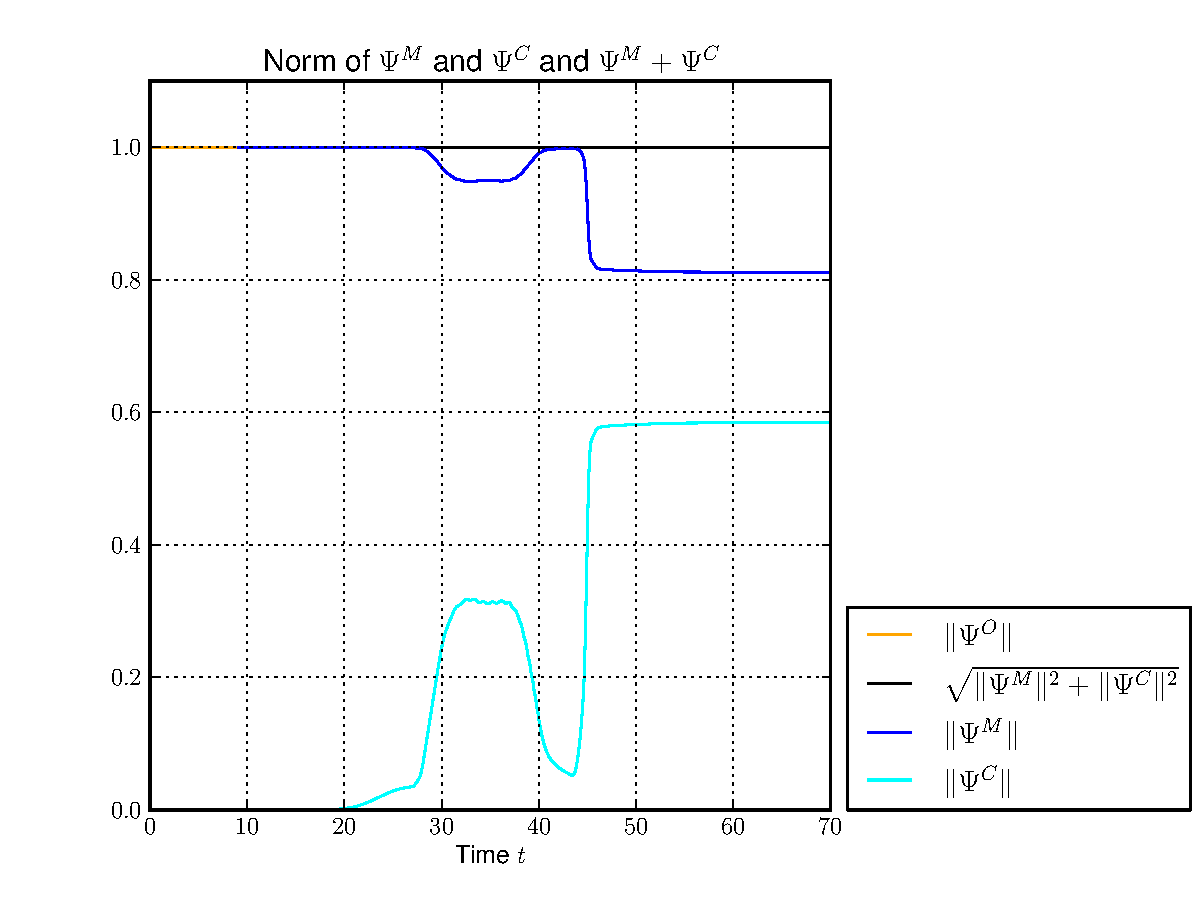
\includegraphics[width=0.5\linewidth]{./figures/eckart_spawn_apost_phi3_K100/norms_compare_sumall_group0.pdf}
  }
  \subfloat[][]{
    \label{fig:spawn_eckart_apost_phi3_K0100_norms_drift}
    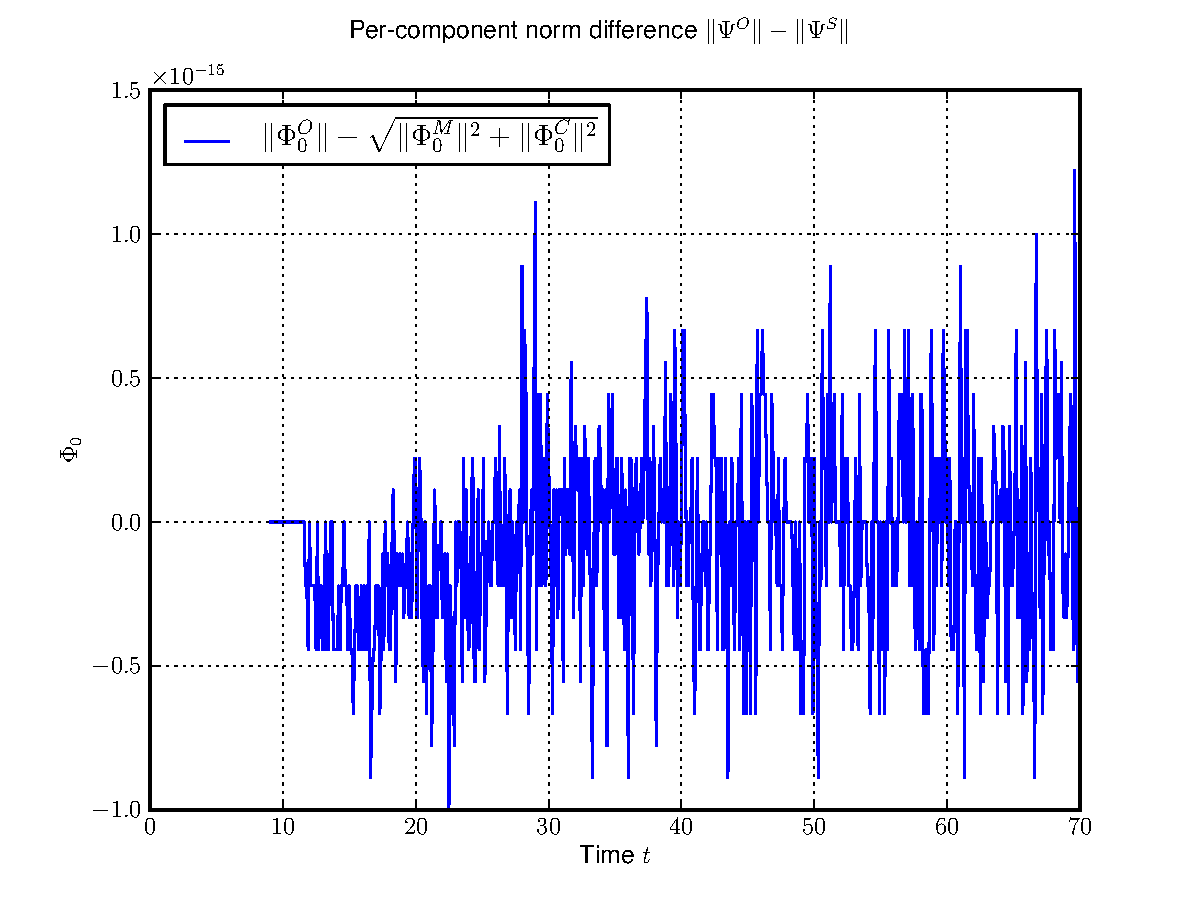
\includegraphics[width=0.5\linewidth]{./figures/eckart_spawn_apost_phi3_K100/norms_compare_components_diff_group0.pdf}
  } \\
  \caption[Norms and norm drift for an aposteriori spawning simulation with lumping]{
  Norms and norm drift for an aposteriori spawning simulation based on the tunneling
  simulation of $\phi_3$. We see perfect norm conservation which has to be expected
  because of the lumping process which is lossless.
  \subref{fig:spawn_eckart_apost_phi3_K050_norms} $\Psi = \phi_3$ and $K_0=50$
  \subref{fig:spawn_eckart_apost_phi3_K050_norms_drift} $\Psi = \phi_3$ and $K_0=50$
  \subref{fig:spawn_eckart_apost_phi3_K075_norms} $\Psi = \phi_3$ and $K_0=75$
  \subref{fig:spawn_eckart_apost_phi3_K075_norms_drift} $\Psi = \phi_3$ and $K_0=75$
  \subref{fig:spawn_eckart_apost_phi3_K0100_norms} $\Psi = \phi_3$ and $K_0=100$
  \subref{fig:spawn_eckart_apost_phi3_K0100_norms_drift} $\Psi = \phi_3$ and $K_0=100$
  \label{fig:spawn_eckart_apost_phi3_norms}
  }
\end{figure}


\begin{figure}[h!]
  \centering
  \subfloat[][]{
    \label{fig:spawn_eckart_apost_phi0_K050_energies_components}
    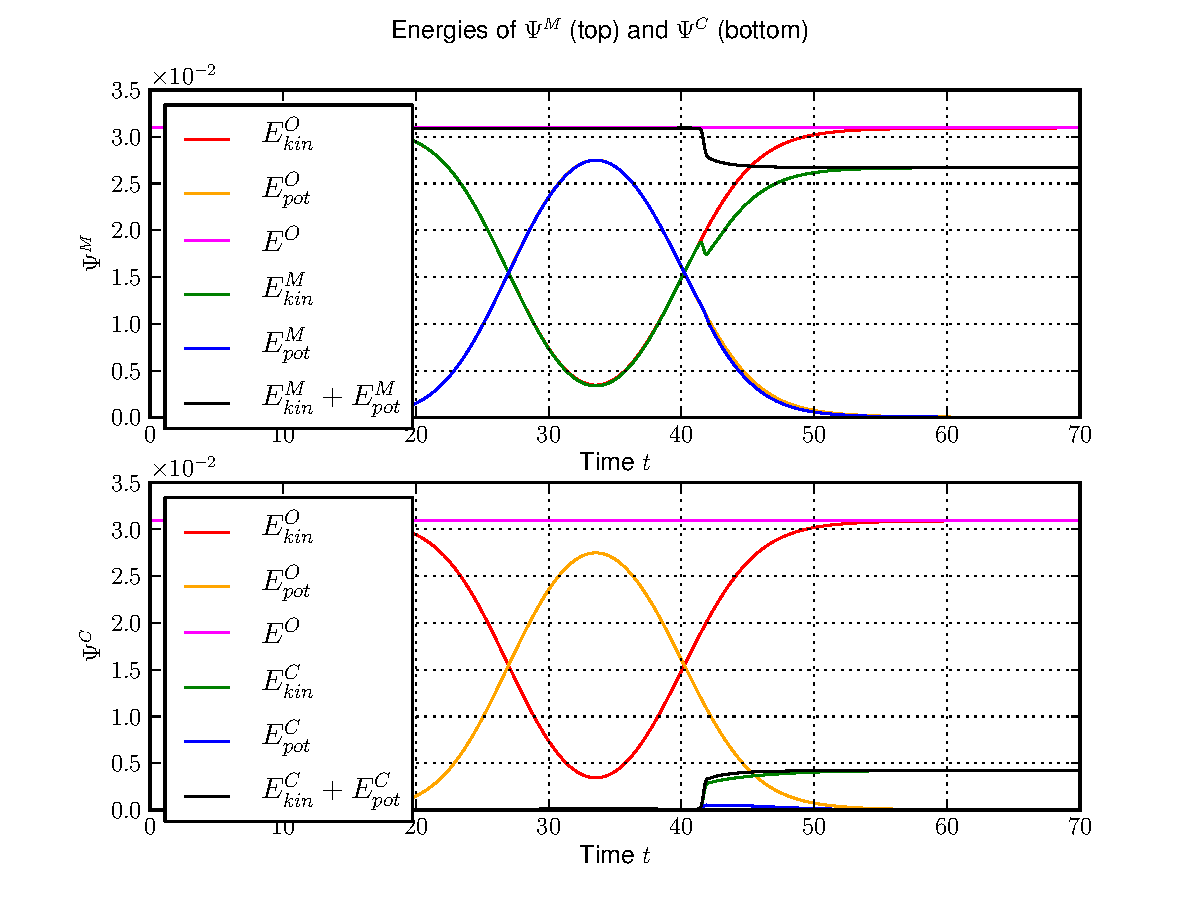
\includegraphics[width=0.5\linewidth]{./figures/eckart_spawn_apost_phi0_K50/energies_compare_packetsum_group0.pdf}
  }
  \subfloat[][]{
    \label{fig:spawn_eckart_apost_phi0_K075_energies_components}
    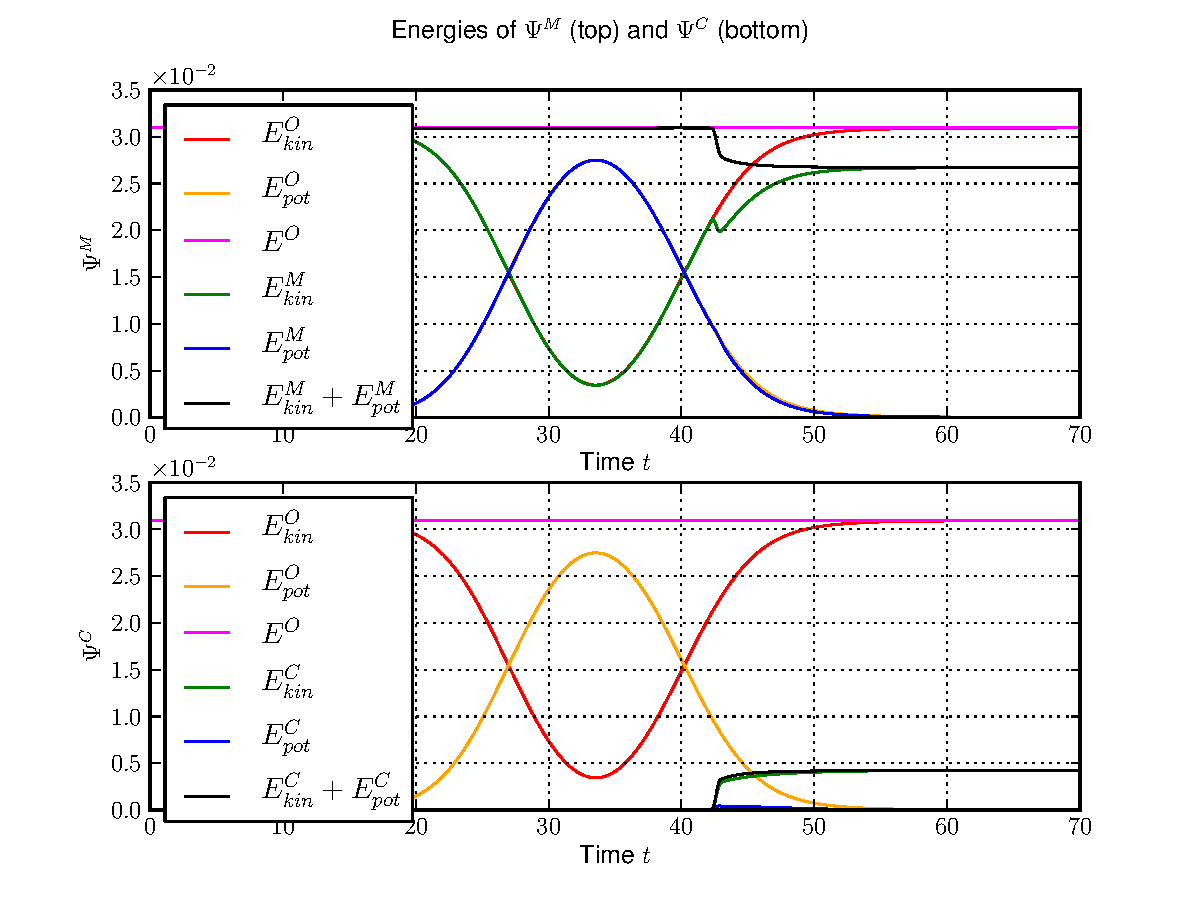
\includegraphics[width=0.5\linewidth]{./figures/eckart_spawn_apost_phi0_K75/energies_compare_packetsum_group0.pdf}
  } \\
  \subfloat[][]{
    \label{fig:spawn_eckart_apost_phi0_K050_energies_sum}
    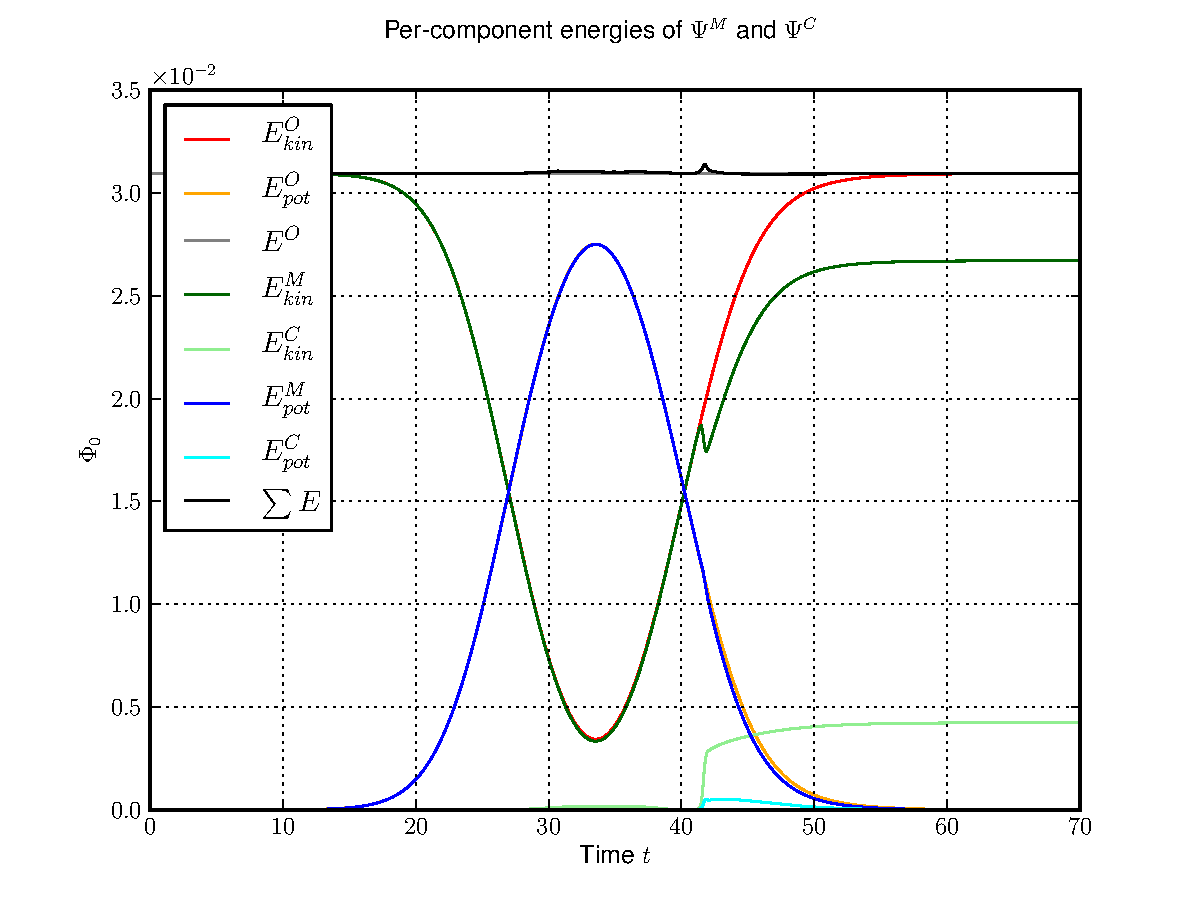
\includegraphics[width=0.5\linewidth]{./figures/eckart_spawn_apost_phi0_K50/energies_compare_components_group0.pdf}
  }
  \subfloat[][]{
    \label{fig:spawn_eckart_apost_phi0_K075_energies_sum}
    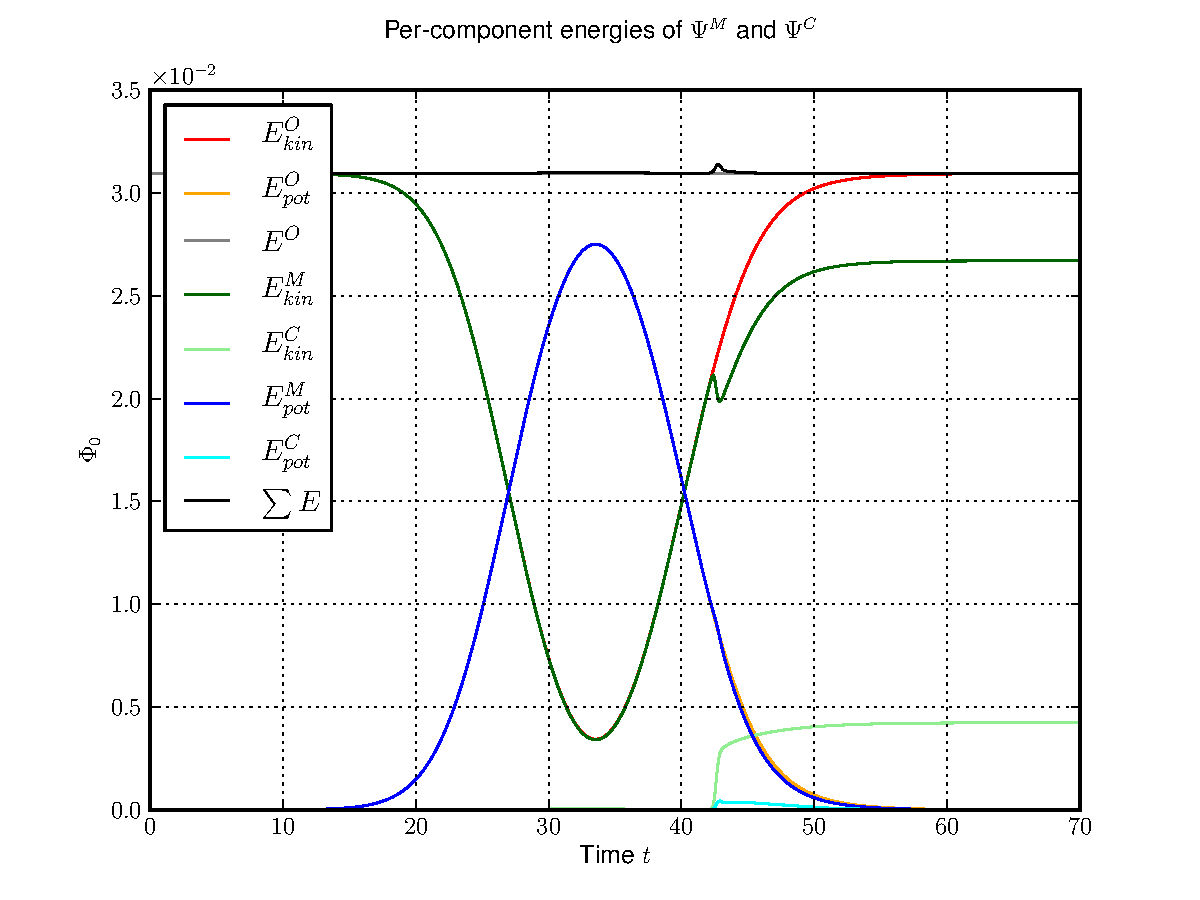
\includegraphics[width=0.5\linewidth]{./figures/eckart_spawn_apost_phi0_K75/energies_compare_components_group0.pdf}
  } \\
  \subfloat[][]{
    \label{fig:spawn_eckart_apost_phi0_K050_energies_drift}
    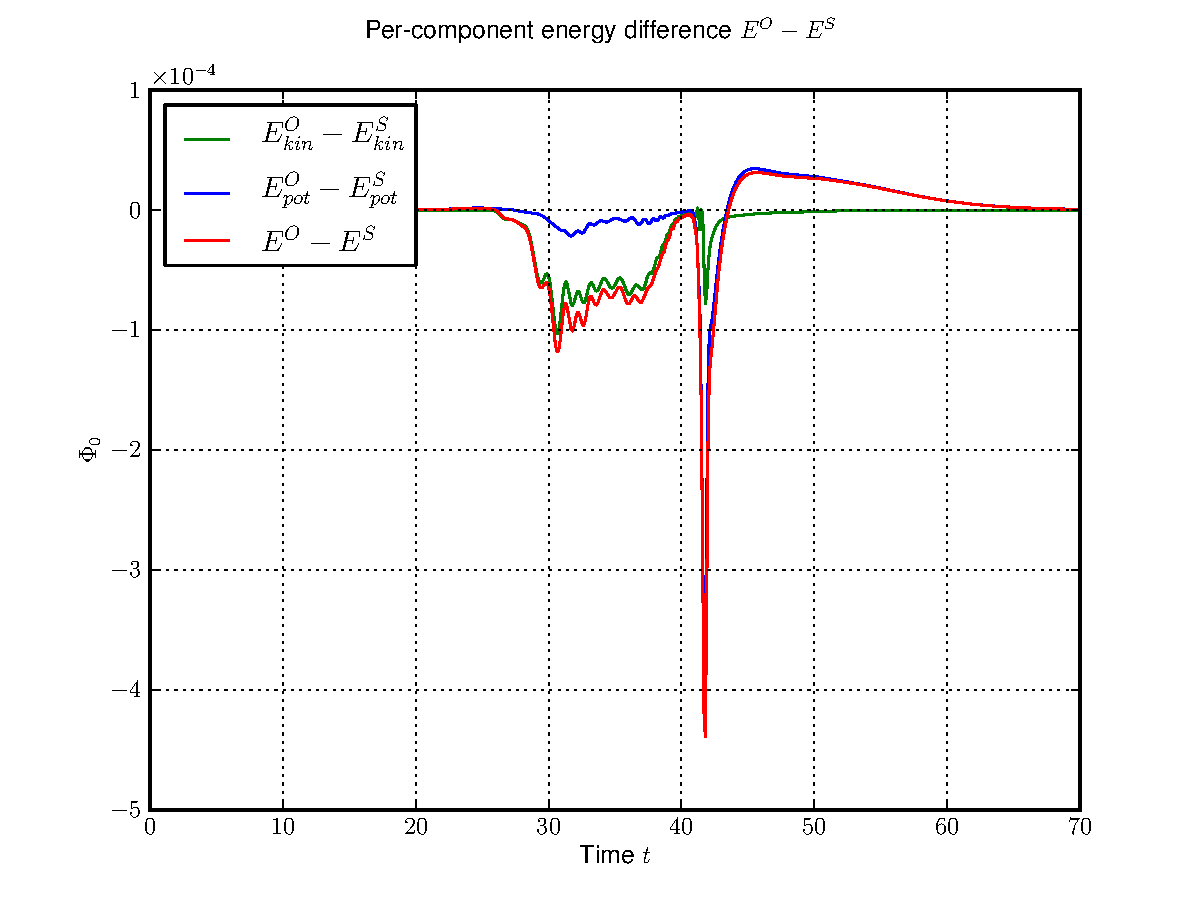
\includegraphics[width=0.5\linewidth]{./figures/eckart_spawn_apost_phi0_K50/energies_compare_components_diff_group0.pdf}
  }
  \subfloat[][]{
    \label{fig:spawn_eckart_apost_phi0_K075_energies_drift}
    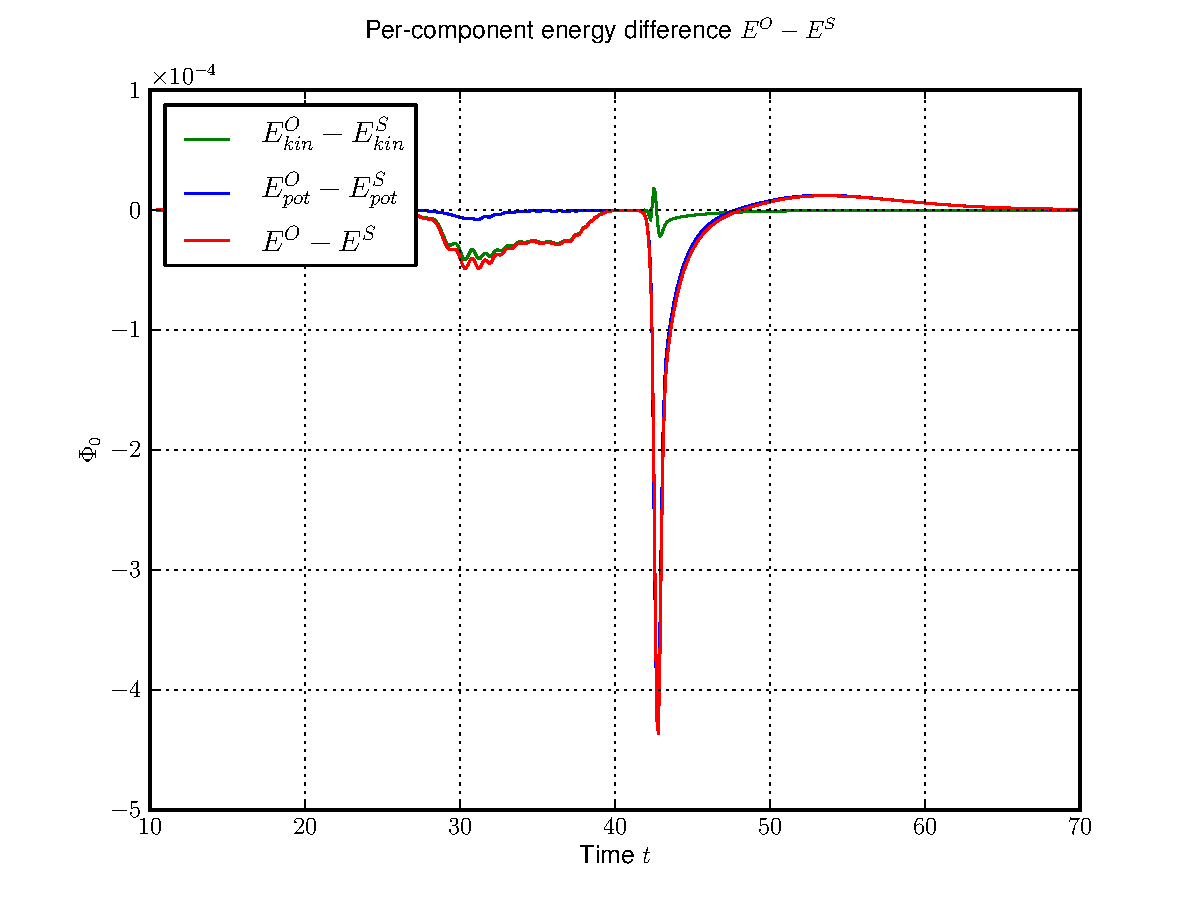
\includegraphics[width=0.5\linewidth]{./figures/eckart_spawn_apost_phi0_K75/energies_compare_components_diff_group0.pdf}
  } \\
  \caption[Energies and energy drift for an aposteriori spawning simulation with lumping]{
  Energies and energy drift for an aposteriori spawning simulation. We try different initial
  for $\Ket{\Psi}$ and several values for $K_0$. Energy conservation for $\Psi = \phi_0$
  is by far good enough but not perfect.
  \subref{fig:spawn_eckart_apost_phi0_K050_energies_components} $\Psi = \phi_0$ and $K_0=50$
  \subref{fig:spawn_eckart_apost_phi0_K075_energies_components} $\Psi = \phi_0$ and $K_0=75$
  \subref{fig:spawn_eckart_apost_phi0_K050_energies_sum} $\Psi = \phi_0$ and $K_0=50$
  \subref{fig:spawn_eckart_apost_phi0_K075_energies_sum} $\Psi = \phi_0$ and $K_0=75$
  \subref{fig:spawn_eckart_apost_phi0_K050_energies_drift} $\Psi = \phi_0$ and $K_0=50$
  \subref{fig:spawn_eckart_apost_phi0_K075_energies_drift} $\Psi = \phi_0$ and $K_0=75$
  \label{fig:spawn_eckart_apost_lump_energies1}
  }
\end{figure}


\begin{figure}[h!]
  \centering
  \subfloat[][]{
    \label{fig:spawn_eckart_apost_phi0_K0100_energies_components}
    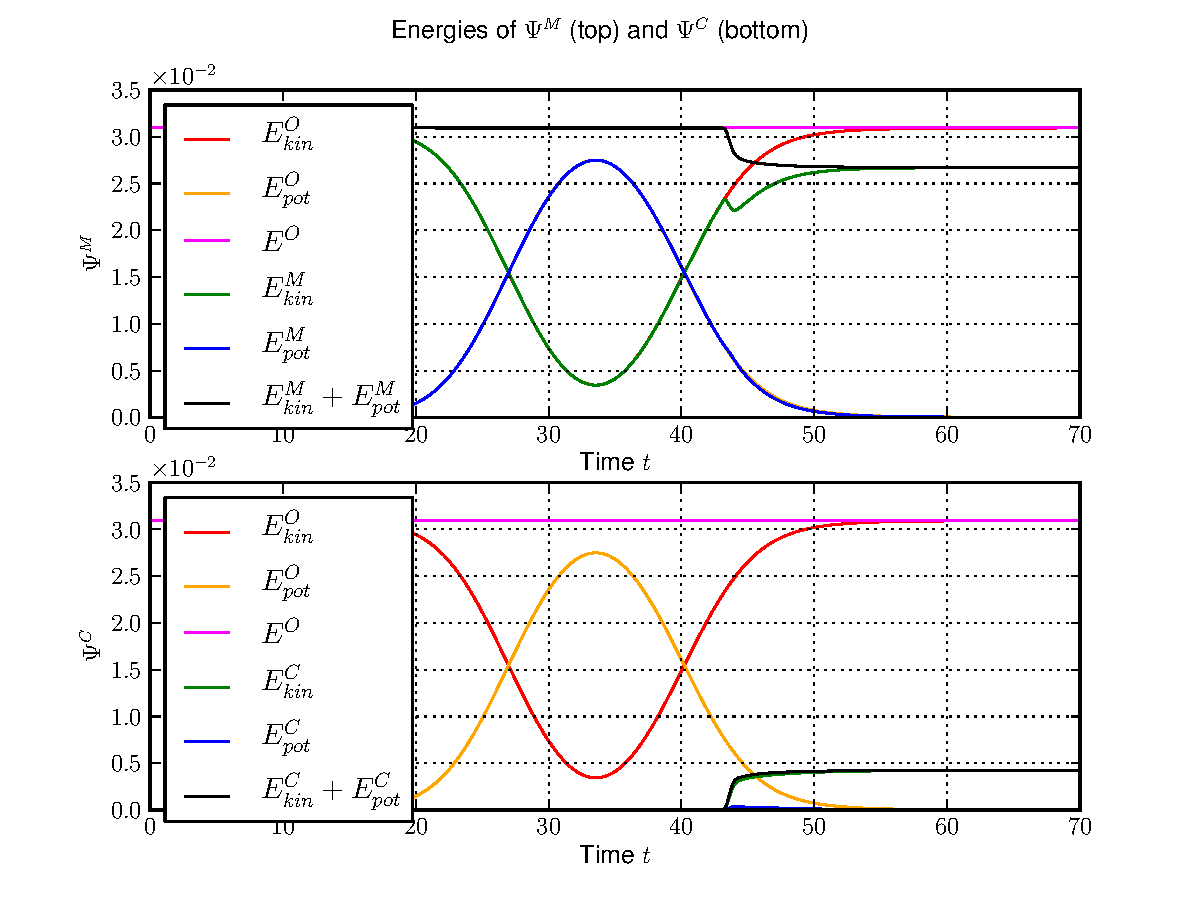
\includegraphics[width=0.5\linewidth]{./figures/eckart_spawn_apost_phi0_K100/energies_compare_packetsum_group0.pdf}
  }
  \subfloat[][]{
    \label{fig:spawn_eckart_apost_phi2_K050_energies_components}
    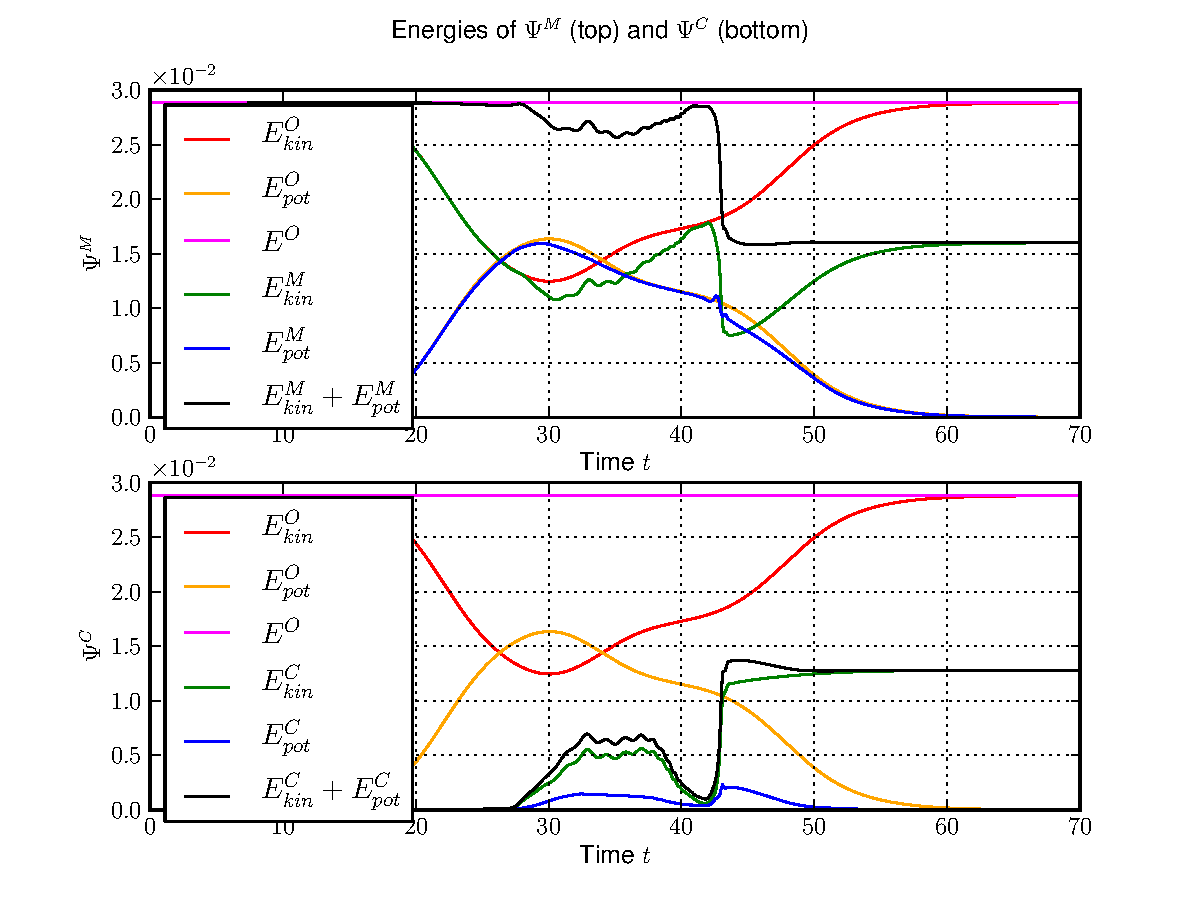
\includegraphics[width=0.5\linewidth]{./figures/eckart_spawn_apost_phi2_K50/energies_compare_packetsum_group0.pdf}
  } \\
  \subfloat[][]{
    \label{fig:spawn_eckart_apost_phi0_K0100_energies_sum}
    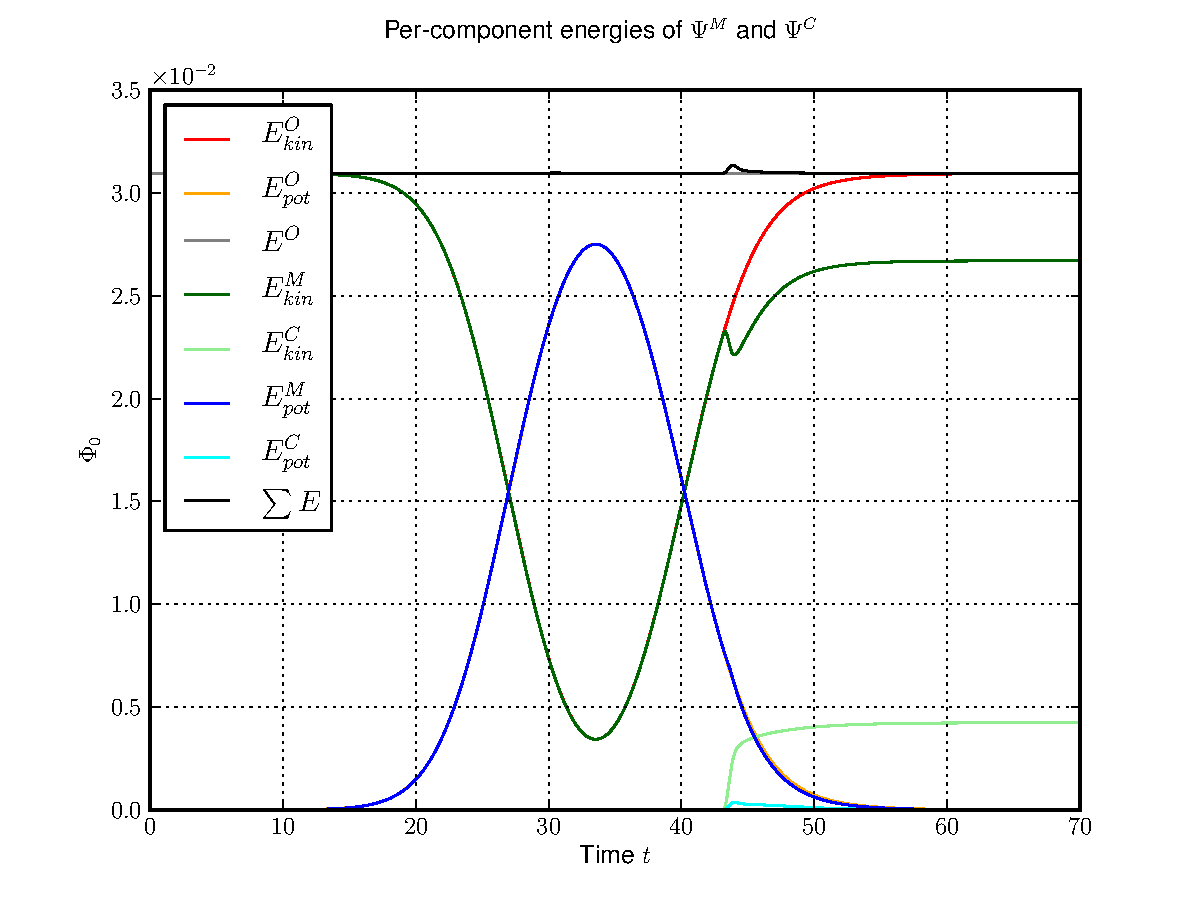
\includegraphics[width=0.5\linewidth]{./figures/eckart_spawn_apost_phi0_K100/energies_compare_components_group0.pdf}
  }
  \subfloat[][]{
    \label{fig:spawn_eckart_apost_phi2_K050_energies_sum}
    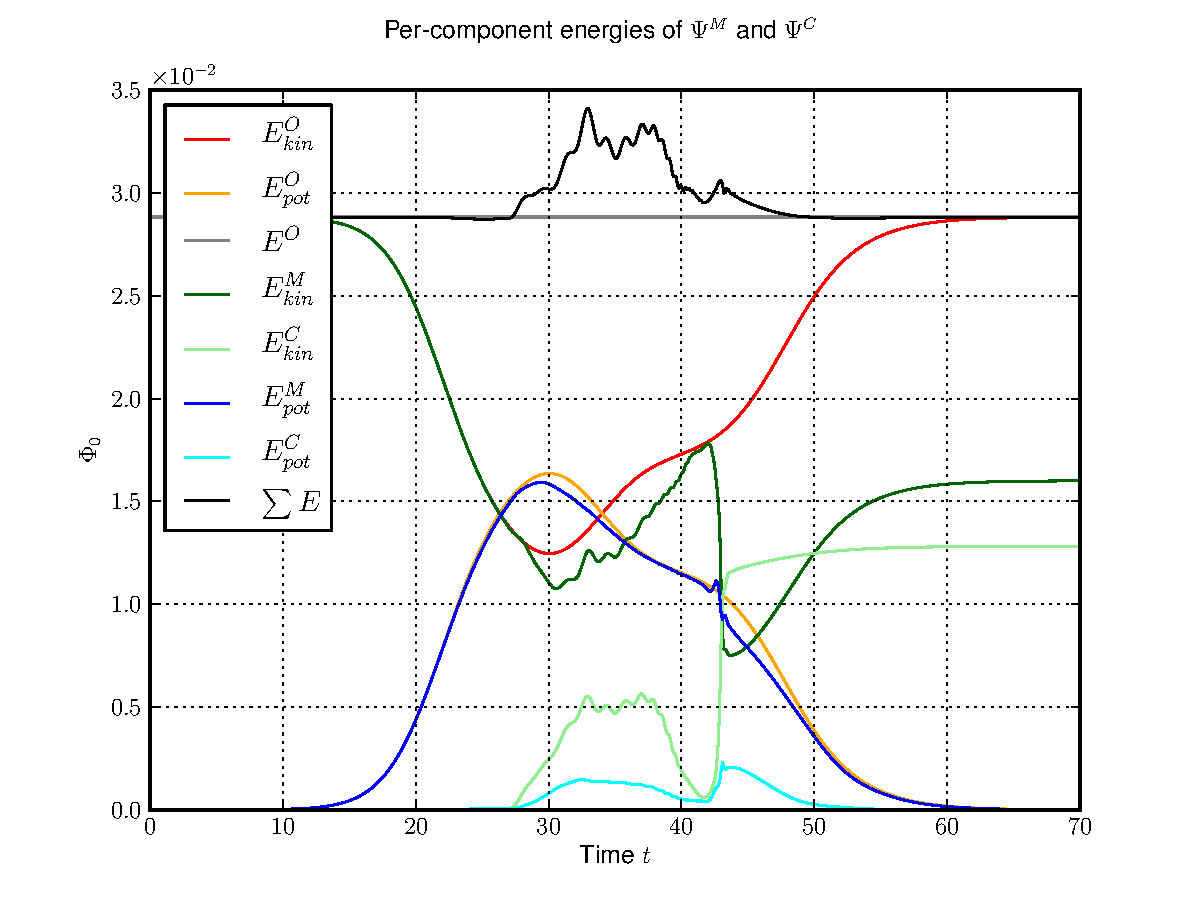
\includegraphics[width=0.5\linewidth]{./figures/eckart_spawn_apost_phi2_K50/energies_compare_components_group0.pdf}
  } \\
  \subfloat[][]{
    \label{fig:spawn_eckart_apost_phi0_K0100_energies_drift}
    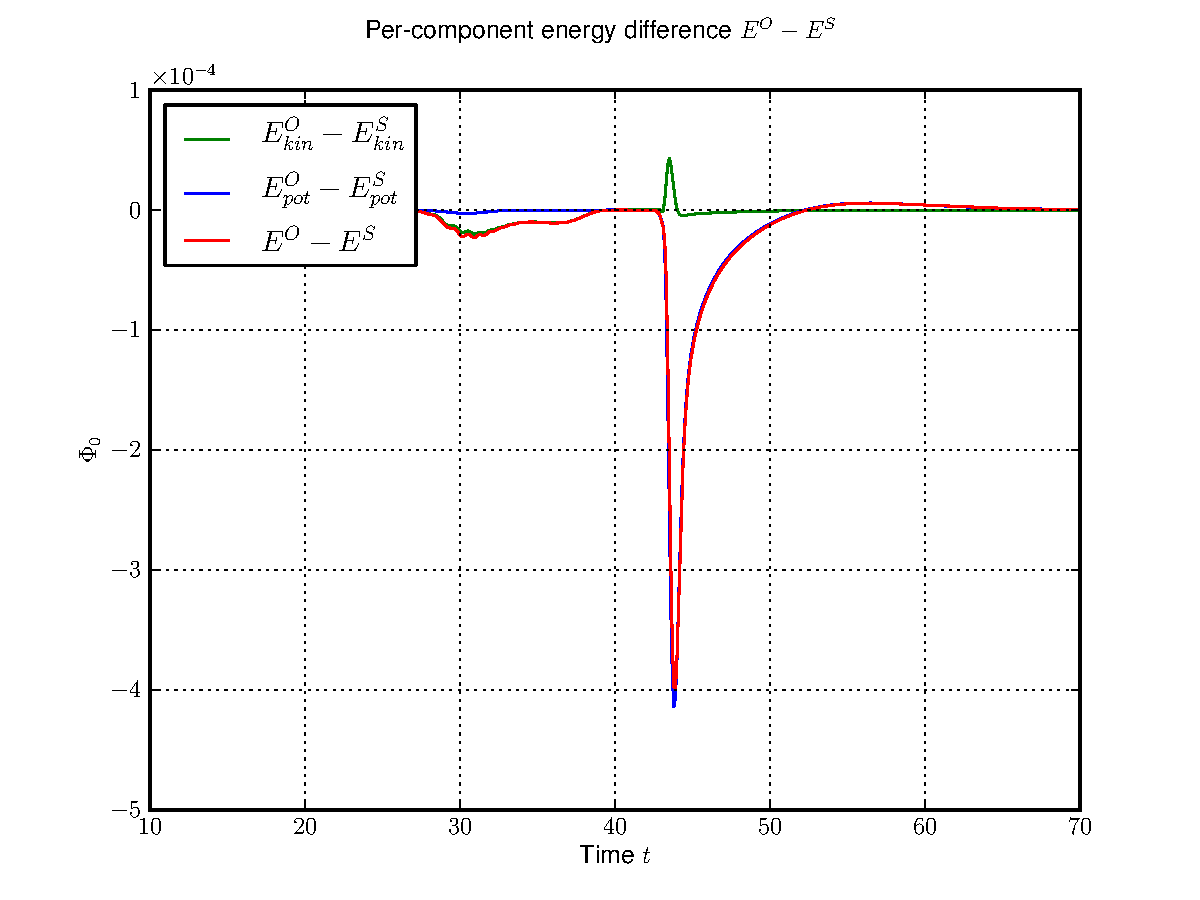
\includegraphics[width=0.5\linewidth]{./figures/eckart_spawn_apost_phi0_K100/energies_compare_components_diff_group0.pdf}
  }
  \subfloat[][]{
    \label{fig:spawn_eckart_apost_phi2_K050_energies_drift}
    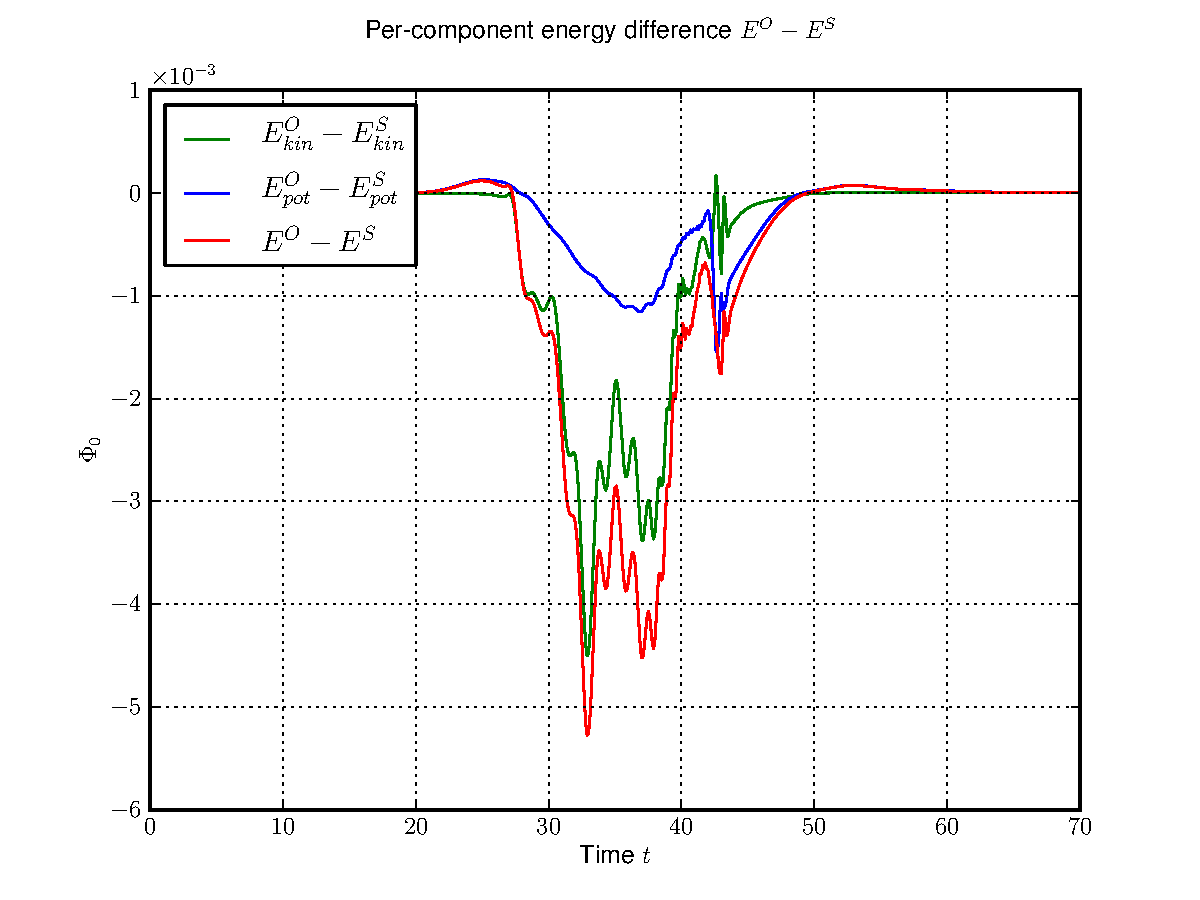
\includegraphics[width=0.5\linewidth]{./figures/eckart_spawn_apost_phi2_K50/energies_compare_components_diff_group0.pdf}
  } \\
  \caption[Energies and energy drift for an aposteriori spawning simulation with lumping]{
  Energies and energy drift for an aposteriori spawning simulation. We try different initial
  for $\Ket{\Psi}$ and several values for $K_0$. Energy conservation for $\Psi = \phi_0$
  is by far good enough but not perfect.
  \subref{fig:spawn_eckart_apost_phi0_K0100_energies_components} $\Psi = \phi_0$ and $K_0=100$
  \subref{fig:spawn_eckart_apost_phi2_K050_energies_components} $\Psi = \phi_2$ and $K_0=50$
  \subref{fig:spawn_eckart_apost_phi0_K0100_energies_sum} $\Psi = \phi_0$ and $K_0=100$
  \subref{fig:spawn_eckart_apost_phi2_K050_energies_sum} $\Psi = \phi_2$ and $K_0=50$
  \subref{fig:spawn_eckart_apost_phi0_K0100_energies_drift} $\Psi = \phi_0$ and $K_0=100$
  \subref{fig:spawn_eckart_apost_phi2_K050_energies_drift} $\Psi = \phi_2$ and $K_0=50$
  \label{fig:spawn_eckart_apost_lump_energies2}
  }
\end{figure}


\begin{figure}[h!]
  \centering
  \subfloat[][]{
    \label{fig:spawn_eckart_apost_phi2_K075_energies_components}
    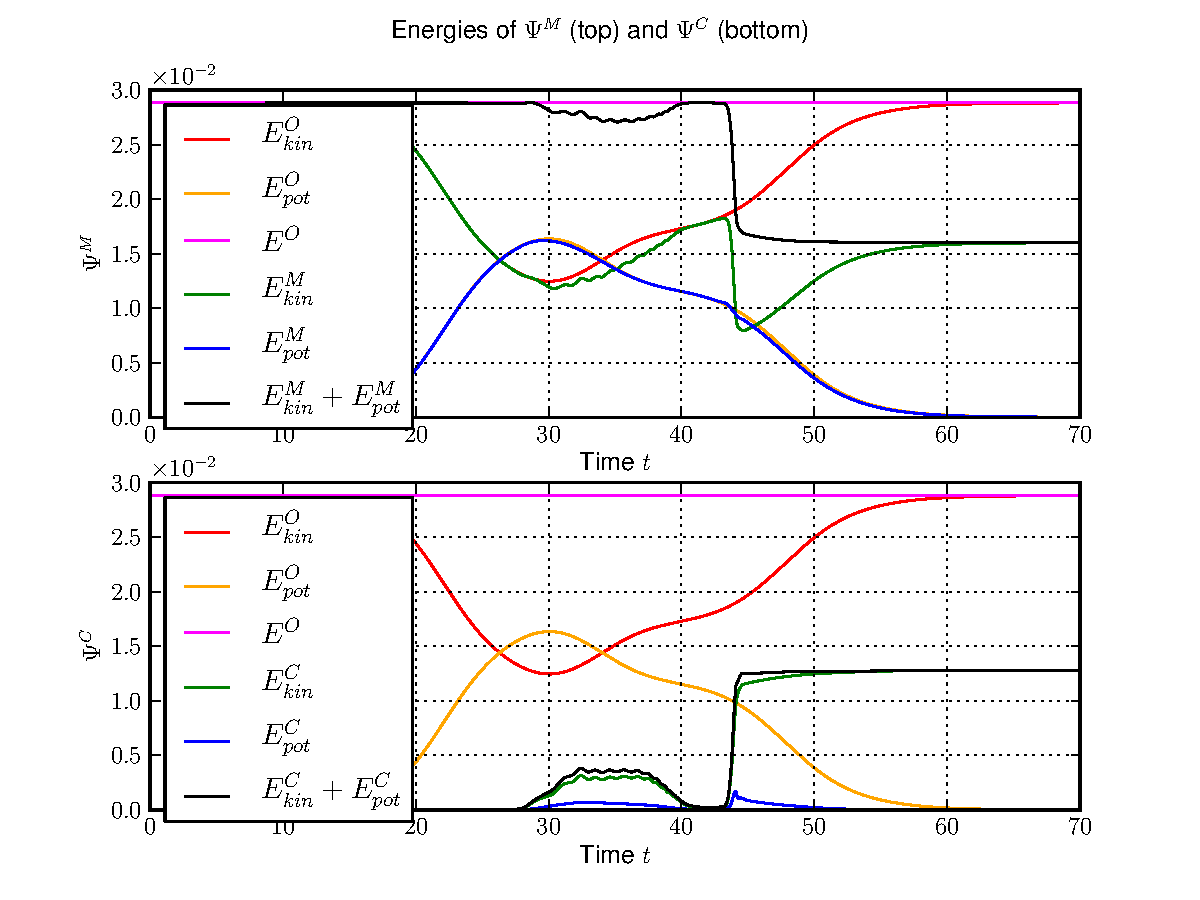
\includegraphics[width=0.5\linewidth]{./figures/eckart_spawn_apost_phi2_K75/energies_compare_packetsum_group0.pdf}
  }
  \subfloat[][]{
    \label{fig:spawn_eckart_apost_phi2_K0100_energies_components}
    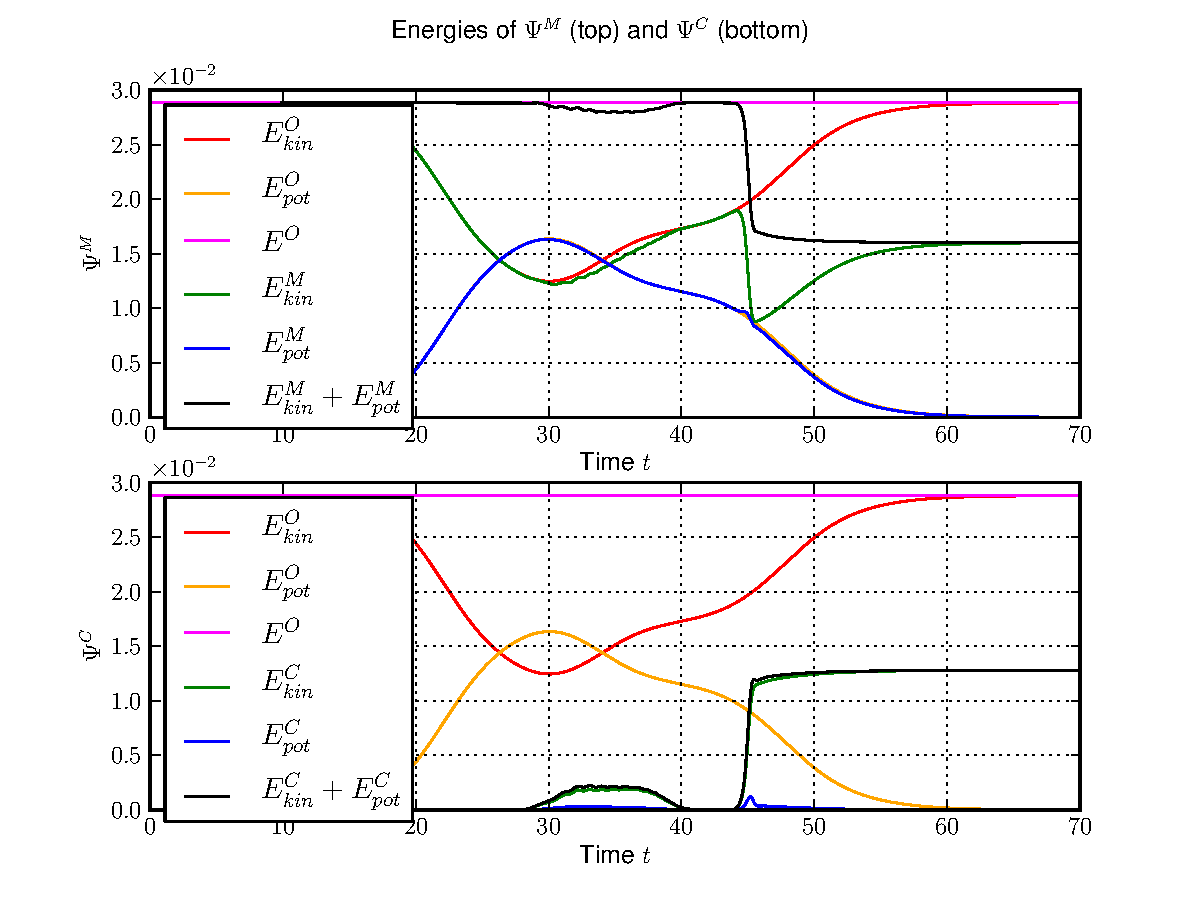
\includegraphics[width=0.5\linewidth]{./figures/eckart_spawn_apost_phi2_K100/energies_compare_packetsum_group0.pdf}
  } \\
  \subfloat[][]{
    \label{fig:spawn_eckart_apost_phi2_K075_energies_sum}
    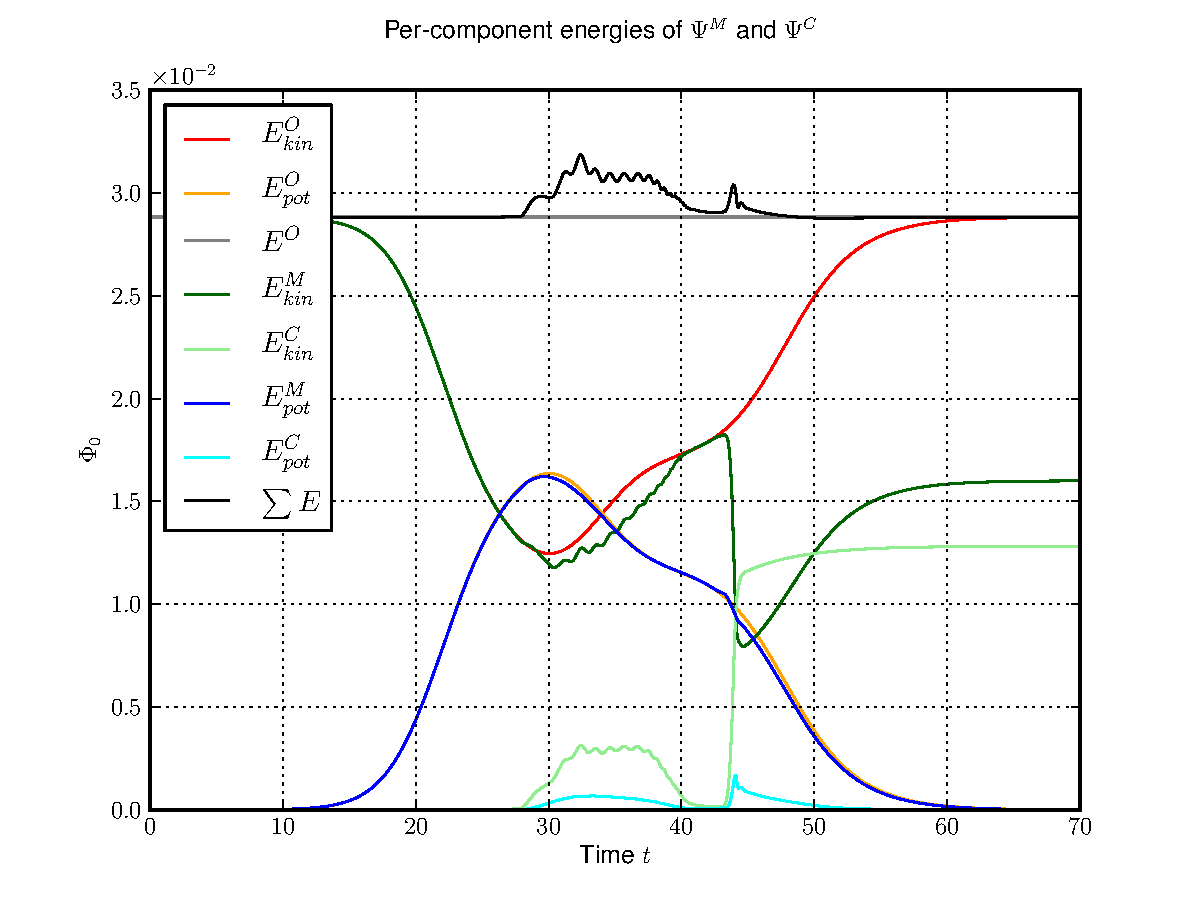
\includegraphics[width=0.5\linewidth]{./figures/eckart_spawn_apost_phi2_K75/energies_compare_components_group0.pdf}
  }
  \subfloat[][]{
    \label{fig:spawn_eckart_apost_phi2_K0100_energies_sum}
    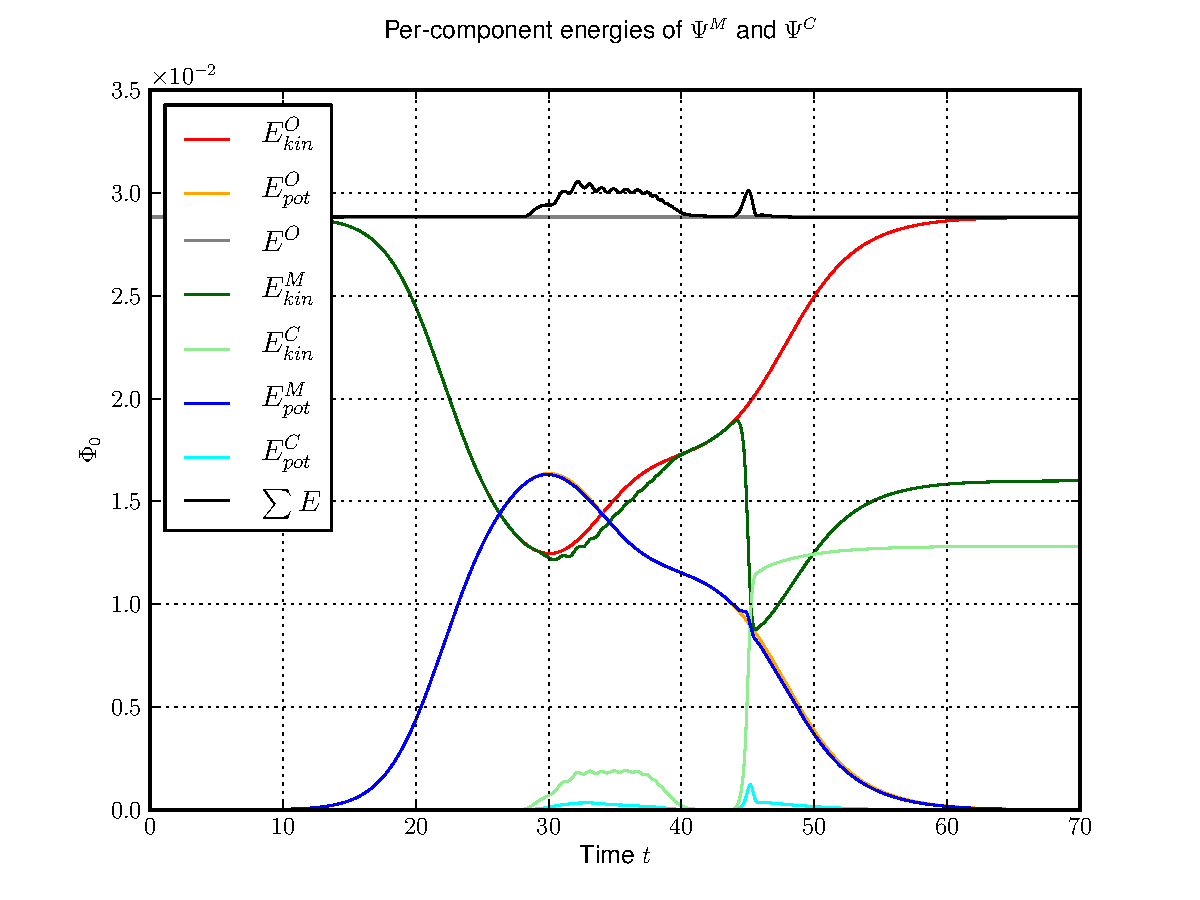
\includegraphics[width=0.5\linewidth]{./figures/eckart_spawn_apost_phi2_K100/energies_compare_components_group0.pdf}
  } \\
  \subfloat[][]{
    \label{fig:spawn_eckart_apost_phi2_K075_energies_drift}
    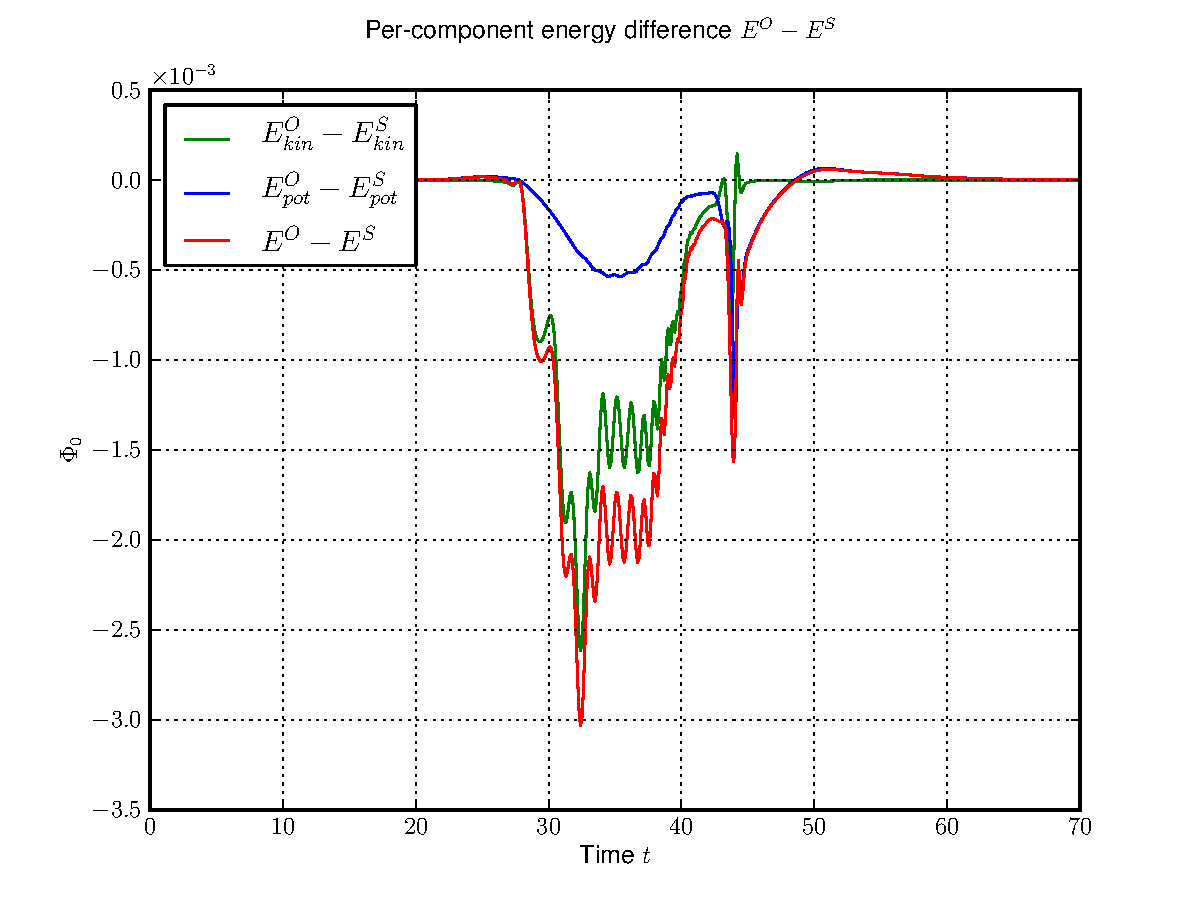
\includegraphics[width=0.5\linewidth]{./figures/eckart_spawn_apost_phi2_K75/energies_compare_components_diff_group0.pdf}
  }
  \subfloat[][]{
    \label{fig:spawn_eckart_apost_phi2_K0100_energies_drift}
    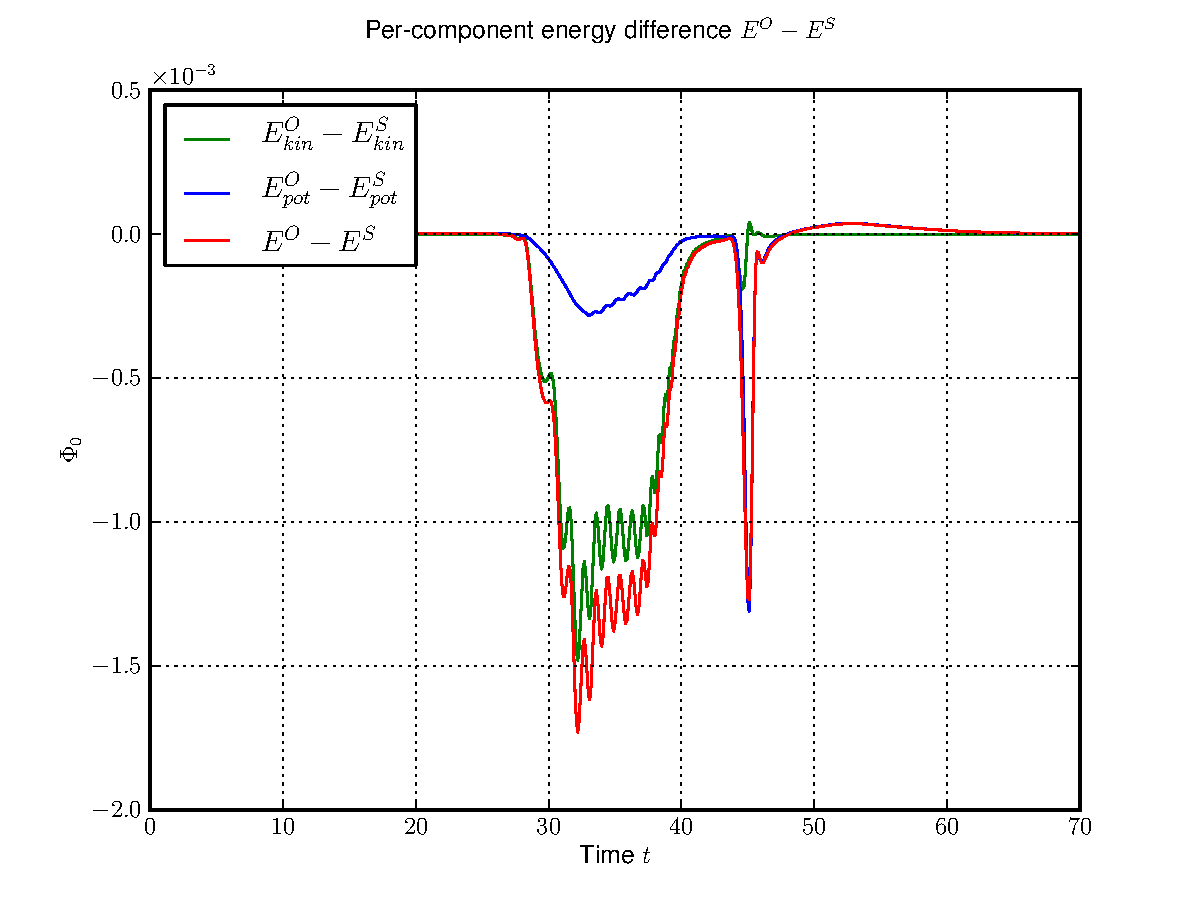
\includegraphics[width=0.5\linewidth]{./figures/eckart_spawn_apost_phi2_K100/energies_compare_components_diff_group0.pdf}
  } \\
  \caption[Energies and energy drift for an aposteriori spawning simulation with lumping]{
  Energies and energy drift for an aposteriori spawning simulation. We try different initial
  for $\Ket{\Psi}$ and several values for $K_0$. Energy conservation is only fulfilled after
  the tunneling event happened and tends to get better with higher $K_0$.
  \subref{fig:spawn_eckart_apost_phi2_K075_energies_components} $\Psi = \phi_2$ and $K_0=75$
  \subref{fig:spawn_eckart_apost_phi2_K0100_energies_components} $\Psi = \phi_2$ and $K_0=100$
  \subref{fig:spawn_eckart_apost_phi2_K075_energies_sum} $\Psi = \phi_2$ and $K_0=75$
  \subref{fig:spawn_eckart_apost_phi2_K0100_energies_sum} $\Psi = \phi_2$ and $K_0=100$
  \subref{fig:spawn_eckart_apost_phi2_K075_energies_drift} $\Psi = \phi_2$ and $K_0=75$
  \subref{fig:spawn_eckart_apost_phi2_K0100_energies_drift} $\Psi = \phi_2$ and $K_0=100$
  \label{fig:spawn_eckart_apost_lump_energies3}
  }
\end{figure}


\begin{figure}[h!]
  \centering
  \subfloat[][]{
    \label{fig:spawn_eckart_apost_phi3_K050_energies_components}
    \includegraphics[width=0.5\linewidth]{./figures/eckart_spawn_apost_phi3_K50/energies_compare_packetsum_group0.pdf}
  }
  \subfloat[][]{
    \label{fig:spawn_eckart_apost_phi3_K075_energies_components}
    \includegraphics[width=0.5\linewidth]{./figures/eckart_spawn_apost_phi3_K75/energies_compare_packetsum_group0.pdf}
  } \\
  \subfloat[][]{
    \label{fig:spawn_eckart_apost_phi3_K050_energies_sum}
    \includegraphics[width=0.5\linewidth]{./figures/eckart_spawn_apost_phi3_K50/energies_compare_components_group0.pdf}
  }
  \subfloat[][]{
    \label{fig:spawn_eckart_apost_phi3_K075_energies_sum}
    \includegraphics[width=0.5\linewidth]{./figures/eckart_spawn_apost_phi3_K75/energies_compare_components_group0.pdf}
  } \\
  \subfloat[][]{
    \label{fig:spawn_eckart_apost_phi3_K050_energies_drift}
    \includegraphics[width=0.5\linewidth]{./figures/eckart_spawn_apost_phi3_K50/energies_compare_components_diff_group0.pdf}
  }
  \subfloat[][]{
    \label{fig:spawn_eckart_apost_phi3_K075_energies_drift}
    \includegraphics[width=0.5\linewidth]{./figures/eckart_spawn_apost_phi3_K75/energies_compare_components_diff_group0.pdf}
  } \\
  \caption[Energies and energy drift for an aposteriori spawning simulation with lumping]{
  Energies and energy drift for an aposteriori spawning simulation. We try different initial
  for $\Ket{\Psi}$ and several values for $K_0$. Energy conservation is only fulfilled after
  the tunneling event happened and tends to get better with higher $K_0$.
  \subref{fig:spawn_eckart_apost_phi3_K050_energies_components} $\Psi = \phi_3$ and $K_0=50$
  \subref{fig:spawn_eckart_apost_phi3_K075_energies_components} $\Psi = \phi_3$ and $K_0=75$
  \subref{fig:spawn_eckart_apost_phi3_K050_energies_sum} $\Psi = \phi_3$ and $K_0=50$
  \subref{fig:spawn_eckart_apost_phi3_K075_energies_sum} $\Psi = \phi_3$ and $K_0=75$
  \subref{fig:spawn_eckart_apost_phi3_K050_energies_drift} $\Psi = \phi_3$ and $K_0=50$
  \subref{fig:spawn_eckart_apost_phi3_K075_energies_drift} $\Psi = \phi_3$ and $K_0=75$
  \label{fig:spawn_eckart_apost_lump_energies4}
  }
\end{figure}


\begin{figure}[h!]
  \centering
  \subfloat[][]{
    \label{fig:spawn_eckart_apost_phi3_K0100_energies_components}
    \includegraphics[width=0.5\linewidth]{./figures/eckart_spawn_apost_phi3_K100/energies_compare_packetsum_group0.pdf}
  } \\
  \subfloat[][]{
    \label{fig:spawn_eckart_apost_phi3_K0100_energies_sum}
    \includegraphics[width=0.5\linewidth]{./figures/eckart_spawn_apost_phi3_K100/energies_compare_components_group0.pdf}
  } \\
  \subfloat[][]{
    \label{fig:spawn_eckart_apost_phi3_K0100_energies_drift}
    \includegraphics[width=0.5\linewidth]{./figures/eckart_spawn_apost_phi3_K100/energies_compare_components_diff_group0.pdf}
  } \\
  \caption[Energies and energy drift for an aposteriori spawning simulation with lumping]{
  Energies and energy drift for an aposteriori spawning simulation. We try different initial
  for $\Ket{\Psi}$ and several values for $K_0$. Energy conservation is only fulfilled after
  the tunneling event happened and tends to get better with higher $K_0$.
  \subref{fig:spawn_eckart_apost_phi3_K0100_energies_components} $\Psi = \phi_3$ and $K_0=100$
  \subref{fig:spawn_eckart_apost_phi3_K0100_energies_sum} $\Psi = \phi_3$ and $K_0=100$
  \subref{fig:spawn_eckart_apost_phi3_K0100_energies_drift} $\Psi = \phi_3$ and $K_0=100$
  \label{fig:spawn_eckart_apost_lump_energies5}
  }
\end{figure}


\begin{figure}[h!]
  \centering
  \includegraphics[width=\the\linewidth]{./figures/eckart_spawn_apost_phi0_K75/wavepacket_parameters_abs_ang_spawned.pdf}
  \caption[The parameter sets $\Pi$ and $\tilde{\Pi}$]{The parameter sets $\Pi$
  (blue) and $\tilde{\Pi}$ (green) estimated from the simulation with $\phi_0$
  plotted versus time. The value of $K_0$ was set to 75.}
  \label{fig:tunnel_spawn_apost_K50_parameters}
\end{figure}

\begin{figure}[h!]
  \centering
  \includegraphics[width=\the\linewidth]{./figures/eckart_spawn_apost_phi2_K75/wavepacket_parameters_abs_ang_spawned.pdf}
  \caption[The parameter sets $\Pi$ and $\tilde{\Pi}$]{The parameter sets $\Pi$
  (blue) and $\tilde{\Pi}$ (green) estimated from the simulation with $\phi_2$
  plotted versus time. The value of $K_0$ was set to 75.
  If we compare this to figure \ref{fig:tunnel_spawn_apost_K50_parameters} we see
  that the green curves differ much in general but little in the important region
  for $t$ larger than about 45.}
\end{figure}

\begin{figure}[h!]
  \centering
  \includegraphics[width=\the\linewidth]{./figures/eckart_spawn_apost_phi3_K75/wavepacket_parameters_abs_ang_spawned.pdf}
  \caption[The parameter sets $\Pi$ and $\tilde{\Pi}$]{The parameter sets $\Pi$
  (blue) and $\tilde{\Pi}$ (green) estimated from the simulation with $\phi_3$
  plotted versus time. The value of $K_0$ was set to 75.
  If we compare this to figure \ref{fig:tunnel_spawn_apost_K50_parameters} we see
  that the green curves differ much in general but little in the important region
  for $t$ larger than about 45.}
\end{figure}


\begin{figure}[h!]
  \centering
  \subfloat[][]{
    \label{fig:spawn_eckart_apost_phi0_K050_spawn_error}
    \includegraphics[width=0.5\linewidth]{./figures/eckart_spawn_apost_phi0_K50/spawn_error_component_norms.pdf}
  }
  \subfloat[][]{
    \label{fig:spawn_eckart_apost_phi2_K050_spawn_error}
    \includegraphics[width=0.5\linewidth]{./figures/eckart_spawn_apost_phi2_K50/spawn_error_component_norms.pdf}
  } \\
  \subfloat[][]{
    \label{fig:spawn_eckart_apost_phi0_K075_spawn_error}
    \includegraphics[width=0.5\linewidth]{./figures/eckart_spawn_apost_phi0_K75/spawn_error_component_norms.pdf}
  }
  \subfloat[][]{
    \label{fig:spawn_eckart_apost_phi2_K075_spawn_error}
    \includegraphics[width=0.5\linewidth]{./figures/eckart_spawn_apost_phi2_K75/spawn_error_component_norms.pdf}
  } \\
  \subfloat[][]{
    \label{fig:spawn_eckart_apost_phi0_K0100_spawn_error}
    \includegraphics[width=0.5\linewidth]{./figures/eckart_spawn_apost_phi0_K100/spawn_error_component_norms.pdf}
  }
  \subfloat[][]{
    \label{fig:spawn_eckart_apost_phi2_K0100_spawn_error}
    \includegraphics[width=0.5\linewidth]{./figures/eckart_spawn_apost_phi2_K100/spawn_error_component_norms.pdf}
  } \\
  \caption[The spawning errors]{The figure shows the spawning error in the $L^2$
  and maximum norm for various initial values $\phi_i$ and different values of $K_0$.
  We see that the choice of $K_0$ is rather unimportant.
  \subref{fig:spawn_eckart_apost_phi0_K050_spawn_error} $\Psi = \phi_0$ and $K_0=50$
  \subref{fig:spawn_eckart_apost_phi2_K050_spawn_error} $\Psi = \phi_2$ and $K_0=50$
  \subref{fig:spawn_eckart_apost_phi0_K075_spawn_error} $\Psi = \phi_0$ and $K_0=75$
  \subref{fig:spawn_eckart_apost_phi2_K075_spawn_error} $\Psi = \phi_2$ and $K_0=75$
  \subref{fig:spawn_eckart_apost_phi0_K0100_spawn_error} $\Psi = \phi_0$ and $K_0=100$
  \subref{fig:spawn_eckart_apost_phi2_K0100_spawn_error} $\Psi = \phi_2$ and $K_0=100$
  \label{fig:spawn_eckart_apost_lump_spawn_error1}
  }
\end{figure}


\begin{figure}[h!]
  \centering
  \subfloat[][]{
    \label{fig:spawn_eckart_apost_phi3_K050_spawn_error}
    \includegraphics[width=0.5\linewidth]{./figures/eckart_spawn_apost_phi3_K100/spawn_error_component_norms.pdf}
  } \\
  \subfloat[][]{
    \label{fig:spawn_eckart_apost_phi3_K075_spawn_error}
    \includegraphics[width=0.5\linewidth]{./figures/eckart_spawn_apost_phi3_K100/spawn_error_component_norms.pdf}
  } \\
  \subfloat[][]{
    \label{fig:spawn_eckart_apost_phi3_K0100_spawn_error}
    \includegraphics[width=0.5\linewidth]{./figures/eckart_spawn_apost_phi3_K100/spawn_error_component_norms.pdf}
  } \\
  \caption[The spawning errors]{The figure shows the spawning error in the $L^2$
  and maximum norm for various initial values $\phi_i$ and different values of $K_0$.
  We see that the choice of $K_0$ is rather unimportant.
  \subref{fig:spawn_eckart_apost_phi3_K050_spawn_error} $\Psi = \phi_3$ and $K_0=50$
  \subref{fig:spawn_eckart_apost_phi3_K075_spawn_error} $\Psi = \phi_3$ and $K_0=75$
  \subref{fig:spawn_eckart_apost_phi3_K0100_spawn_error} $\Psi = \phi_3$ and $K_0=100$
  \label{fig:spawn_eckart_apost_lump_spawn_error2}
  }
\end{figure}


\FloatBarrier
\section{Spawning using the projection method}

In this section we show several results of the projection method used for the change
of basis during the spawning process. All results take the tunneling simulation with
a $\phi_0$ as the base and set $K_0 = 50$ for parameter estimation. We then try to
project on differently many basis functions $\{\tilde{\phi}_k\}_{k=0}^{\mu-1}$. In
general we see an increase in the goodness of all properties with larger $\mu$. The
results are also better than what we got with the lumping method in the last section.
This is exceedingly true for short times right after tunneling happened because
at this time the transmitted part has not yet the shape of a Gaussian. This then
shows up for larger times and holds only asymptotically. Hence we can improve the results
if we drop the assumption that the transmitted part is always a Gaussian.


\begin{figure}[h!]
  \centering
  \includegraphics[width=\the\linewidth]{./figures/eckart_phi0_spawn_project_K50_bs6/wavepacket_coefficients_spawn_first.png}
  \caption[The first five coefficients $c_i$ of the original and $\tilde{c_i}$ of the spawned packet]
  {The figure shows the first five coefficients $c_i$ of the original and $\tilde{c_i}$ of the spawned packet.
  The red and black curves are the absolute values, the others are real and imaginary parts. If we project for example
  only on the first three basis functions, then the black lines for $\tilde{c_3}$ and $\tilde{c_4}$ would be
  identical zero.}
\end{figure}


\begin{figure}[h!]
  \centering
  \subfloat[][]{
    \label{fig:tunnel_spawn_project_K50_bs1_norms}
    \includegraphics[width=0.5\linewidth]{./figures/eckart_phi0_spawn_project_K50_bs1/norms_compare_components_group0.png}
  }
  \subfloat[][]{
    \label{fig:tunnel_spawn_project_K50_bs3_norms}
    \includegraphics[width=0.5\linewidth]{./figures/eckart_phi0_spawn_project_K50_bs3/norms_compare_components_group0.png}
  } \\
  \subfloat[][]{
    \label{fig:tunnel_spawn_project_K50_bs6_norms}
    \includegraphics[width=0.5\linewidth]{./figures/eckart_phi0_spawn_project_K50_bs6/norms_compare_components_group0.png}
  }
  \subfloat[][]{
    \label{fig:tunnel_spawn_project_K50_bs12_norms}
    \includegraphics[width=0.5\linewidth]{./figures/eckart_phi0_spawn_project_K50_bs12/norms_compare_components_group0.png}
  } \\
  \caption[Norms of the original and spawned wavepackets using the projection spawning method]{
  The panels show the norms of the original wavepacket (suffix O), the spawned
  wavepacket (suffix C) and the remainder packet (suffix M).
  We find increasing norm conservation (black curve is overall energy) during the spawning
  process for increasing values of the projection spawning parameter $\mu$.
  (This parameter is the number of basis functions we project onto.)
  This is a difference to the spawning using lumping where we always have perfect
  norm conservation.
  \subref{fig:tunnel_spawn_project_K50_bs1_norms} Projection spawning parameter $\mu = 1$.
  \subref{fig:tunnel_spawn_project_K50_bs3_norms} Projection spawning parameter $\mu = 3$.
  \subref{fig:tunnel_spawn_project_K50_bs6_norms} Projection spawning parameter $\mu = 6$.
  \subref{fig:tunnel_spawn_project_K50_bs12_norms} Projection spawning parameter $\mu = 12$.
  \label{fig:tunnel_spawn_project_K50_spawn_norms}
  }
\end{figure}


\begin{figure}[h!]
  \centering
  \subfloat[][]{
    \label{fig:tunnel_spawn_project_K50_bs1_norms_drift}
    \includegraphics[width=0.5\linewidth]{./figures/eckart_phi0_spawn_project_K50_bs1/norms_compare_components_diff_group0.png}
  }
  \subfloat[][]{
    \label{fig:tunnel_spawn_project_K50_bs3_norms_drift}
    \includegraphics[width=0.5\linewidth]{./figures/eckart_phi0_spawn_project_K50_bs3/norms_compare_components_diff_group0.png}
  } \\
  \subfloat[][]{
    \label{fig:tunnel_spawn_project_K50_bs6_norms_drift}
    \includegraphics[width=0.5\linewidth]{./figures/eckart_phi0_spawn_project_K50_bs6/norms_compare_components_diff_group0.png}
  }
  \subfloat[][]{
    \label{fig:tunnel_spawn_project_K50_bs12_norms_drift}
    \includegraphics[width=0.5\linewidth]{./figures/eckart_phi0_spawn_project_K50_bs12/norms_compare_components_diff_group0.png}
  } \\
  \caption[Difference of the norms of the original and spawned wavepackets using the projection spawning method]{
  The panels show the difference of the norms of the original wavepacket (suffix O), the spawned
  wavepacket (suffix C) and the remainder packet (suffix M). We find increasing norm
  conservation for larger values of the projection spawning parameter $\mu$. (This
  parameter is the number of basis functions we project onto.) This is a difference
  to the spawning using lumping where we always have perfect norm conservation.
  \subref{fig:tunnel_spawn_project_K50_bs1_norms_drift} Projection spawning parameter $\mu = 1$.
  \subref{fig:tunnel_spawn_project_K50_bs3_norms_drift} Projection spawning parameter $\mu = 3$.
  \subref{fig:tunnel_spawn_project_K50_bs6_norms_drift} Projection spawning parameter $\mu = 6$.
  \subref{fig:tunnel_spawn_project_K50_bs12_norms_drift} Projection spawning parameter $\mu = 12$.
  \label{fig:tunnel_spawn_project_K50_spawn_norms_drift}
  }
\end{figure}


\begin{figure}[h!]
  \centering
  \subfloat[][]{
    \label{fig:tunnel_spawn_project_K50_bs1_energies}
    \includegraphics[width=0.5\linewidth]{./figures/eckart_phi0_spawn_project_K50_bs1/energies_compare_components_group0.png}
  }
  \subfloat[][]{
    \label{fig:tunnel_spawn_project_K50_bs3_energies}
    \includegraphics[width=0.5\linewidth]{./figures/eckart_phi0_spawn_project_K50_bs3/energies_compare_components_group0.png}
  } \\
  \subfloat[][]{
    \label{fig:tunnel_spawn_project_K50_bs6_energies}
    \includegraphics[width=0.5\linewidth]{./figures/eckart_phi0_spawn_project_K50_bs6/energies_compare_components_group0.png}
  }
  \subfloat[][]{
    \label{fig:tunnel_spawn_project_K50_bs12_energies}
    \includegraphics[width=0.5\linewidth]{./figures/eckart_phi0_spawn_project_K50_bs12/energies_compare_components_group0.png}
  } \\
  \caption[Energies of the original and spawned wavepackets using the projection spawning method]{
  The panels show the kinetic and potential energies of the original wavepacket (suffix O),
  the spawned wavepacket (suffix C) and the remainder packet (suffix M).
  We find increasing energy conservation (black curve is overall energy) during the spawning
  process for increasing values of the projection spawning parameter $\mu$.
  (This parameter is the number of basis functions we project onto.)
  \subref{fig:tunnel_spawn_project_K50_bs1_energies} Projection spawning parameter $\mu = 1$.
  \subref{fig:tunnel_spawn_project_K50_bs3_energies} Projection spawning parameter $\mu = 3$.
  \subref{fig:tunnel_spawn_project_K50_bs6_energies} Projection spawning parameter $\mu = 6$.
  \subref{fig:tunnel_spawn_project_K50_bs12_energies} Projection spawning parameter $\mu = 12$.
  \label{fig:tunnel_spawn_project_K50_spawn_energies}
  }
\end{figure}


\begin{figure}[h!]
  \centering
  \subfloat[][]{
    \label{fig:tunnel_spawn_project_K50_bs1_energies_drift}
    \includegraphics[width=0.5\linewidth]{./figures/eckart_phi0_spawn_project_K50_bs1/energies_compare_components_diff_group0.png}
  }
  \subfloat[][]{
    \label{fig:tunnel_spawn_project_K50_bs3_energies_drift}
    \includegraphics[width=0.5\linewidth]{./figures/eckart_phi0_spawn_project_K50_bs3/energies_compare_components_diff_group0.png}
  } \\
  \subfloat[][]{
    \label{fig:tunnel_spawn_project_K50_bs6_energies_drift}
    \includegraphics[width=0.5\linewidth]{./figures/eckart_phi0_spawn_project_K50_bs6/energies_compare_components_diff_group0.png}
  }
  \subfloat[][]{
    \label{fig:tunnel_spawn_project_K50_bs12_energies_drift}
    \includegraphics[width=0.5\linewidth]{./figures/eckart_phi0_spawn_project_K50_bs12/energies_compare_components_diff_group0.png}
  } \\
  \caption[Energy difference of the original and spawned wavepackets using the projection spawning method]{
  The panels show the difference of the kinetic and potential energies between the
  original wavepacket (suffix O), the spawned wavepacket (suffix C) and the remainder
  packet (suffix M). We find increasing energy conservation for larger values of the
  projection spawning parameter $\mu$ (This parameter is the number of basis functions we project onto.)
  \subref{fig:tunnel_spawn_project_K50_bs1_energies_drift} Projection spawning parameter $\mu = 1$.
  \subref{fig:tunnel_spawn_project_K50_bs3_energies_drift} Projection spawning parameter $\mu = 3$.
  \subref{fig:tunnel_spawn_project_K50_bs6_energies_drift} Projection spawning parameter $\mu = 6$.
  \subref{fig:tunnel_spawn_project_K50_bs12_energies_drift} Projection spawning parameter $\mu = 12$.
  \label{fig:tunnel_spawn_project_K50_spawn_energies_drift}
  }
\end{figure}


\begin{figure}[h!]
  \centering
  \subfloat[][]{
    \label{fig:tunnel_spawn_project_K50_bs1_spawn_error}
    \includegraphics[width=0.5\linewidth]{./figures/eckart_phi0_spawn_project_K50_bs1/spawn_error_norm.png}
  }
  \subfloat[][]{
    \label{fig:tunnel_spawn_project_K50_bs3_spawn_error}
    \includegraphics[width=0.5\linewidth]{./figures/eckart_phi0_spawn_project_K50_bs3/spawn_error_norm.png}
  } \\
  \subfloat[][]{
    \label{fig:tunnel_spawn_project_K50_bs6_spawn_error}
    \includegraphics[width=0.5\linewidth]{./figures/eckart_phi0_spawn_project_K50_bs6/spawn_error_norm.png}
  }
  \subfloat[][]{
    \label{fig:tunnel_spawn_project_K50_bs12_spawn_error}
    \includegraphics[width=0.5\linewidth]{./figures/eckart_phi0_spawn_project_K50_bs12/spawn_error_norm.png}
  } \\
  \caption[Norm of the spawn error with the projection spawning method]{
  The panels show the norm of the spawn error measured in $L^2$ and maximum norm. We see
  that we can reduce the error with increasing projection spawning parameter $\mu$. (This parameter
  is the number of basis functions we project onto.)
  \subref{fig:tunnel_spawn_project_K50_bs1_spawn_error} Projection spawning parameter $\mu = 1$.
  \subref{fig:tunnel_spawn_project_K50_bs3_spawn_error} Projection spawning parameter $\mu = 3$.
  \subref{fig:tunnel_spawn_project_K50_bs6_spawn_error} Projection spawning parameter $\mu = 6$.
  \subref{fig:tunnel_spawn_project_K50_bs12_spawn_error} Projection spawning parameter $\mu = 12$.
  \label{fig:tunnel_spawn_project_K50_spawn_error}
  }
\end{figure}


One conclusion of this section is that the lumping method works (and is also very
fast to compute) but the projection method is superior in most applications. The
reason for this is that we seldom have a pure basis function $\phi_k$ as the master
fragment for which spawning is tried. And even for very slight deviations from
the pure form the projection method is better. (Remember that although we theoretically
expect a Gaussian after tunneling this result holds only for asymptotically large
times. Contrary to that our simulation takes place in short up to moderately long times after
the tunneling event.) For example this also happens in simulations where the mother
fragment has roughly the shape of a $\phi_2$ but with one of its peaks is higher
than the others.


\FloatBarrier
\section{Spawning and propagation}
\label{sec:spawn_propag_tunnel}

In the last section we looked at many different examples of tunneling simulations.
By now we have got an idea how spawning works in practice and saw that it works
quite well although there are some difficulties and possibilities for improvement.
As we wrote earlier the aposteriori spawning process is only good for gaining insight
in the spawning process itself but gives no improvements otherwise. Hence we will investigate
in this section how we can take the full advantage of spawning for better and faster
simulations.

The key point is that we in principle do the time propagation as usual but now and
then check if some condition is fulfilled which then triggers spawning. After
a spawning event occurred we proceed with the normal time propagation again but
now we have one more packet to propagate. We should stress that spawning events
are very rare. And thus there is little risk of ending up with dozens of packets.
We call this combined algorithm the \emph{spawning propagation method}.

The criterion for spawning is difficult to choose. There are many possibilities,
some of them work well in theory but are problematic to implement and vice versa.
The most simple one is probably to introduce a threshold $\tau$ and monitor the
norms of the mother fragments $w$ which are candidates for spawning. If then the
norm $\Braket{w|w}$ gets larger than $\tau$ this triggers the spawning process once.

We concentrate on this criterion because it is simple both to understand and to
implement. But we will see later in the examples that there are some pitfalls.

The algorithm \ref{al:spawning_propagation} shows the course layout of the
concepts described in the paragraph above. It is a simplified version in the
sense that we start with a single wavepacket $\Ket{\Psi}$ and presume we will
fulfill  the spawning criterion only once. Hence we will end up with only
two wavepackets $\Ket{\Psi_0}$ and $\Ket{\Psi_1}$. For both of these the criterion
will never be true again. To see this also compare to the images \ref{fig:spawning_propagation_intro1},
\ref{fig:spawning_propagation_intro2} and \ref{fig:spawning_propagation_intro3}.
The parts on propagation left out and can be found in the references given,
copying over and plugging in these algorithms is obvious. This is exactly the
situation in a simple tunneling simulation, thus we can apply this algorithm
to such a tunneling problem. For more advanced cases like avoided crossings
we will need to extend the algorithm later on in the next chapters.


\begin{algorithm}
\caption{Spawning propagation method (simplified)}
\label{al:spawning_propagation}
\begin{algorithmic}
  \REQUIRE A series $t$ consisting of timesteps $\{\tau_0, \ldots, \tau_{\text{max}}\}$
  \REQUIRE The potential $V\ofs{x}$
  \REQUIRE The initial wavepacket $\Ket{\Psi\ofs{t=\tau_o}}$ with its coefficients $\{c_k\}_{k=0}^{K-1}$
  \REQUIRE The value of $0 \leq K_0 \leq K-1$
  \REQUIRE A spawn threshold $\tau$
  \FORALL{$\tau_i \in t$}
    \STATE // Decompose $\Psi$ according to \eqref{eq:decompose_psi_tunnel} with high-frequency part $w$ of $\Psi$
    \STATE $v \assign \sum_{k=0}^{K_0-1} c_k \phi_k$
    \STATE $w \assign \sum_{k=K_0}^{K-1} c_k \phi_k$
    \STATE // Check the spawning criterion
    \IF{$\Braket{w|w} \geq \tau^2$}
      \STATE // Perform spawning procedure
      \STATE // Estimate the parameters of the fragment by algorithm \ref{al:parameter_estimation}
      \STATE $\tilde{\Pi} \assign \textbf{estimate\_parameters}(w)$
      \STATE // Move the fragment $w$ to the new basis by either algorithm \ref{al:lumping_method} or \ref{al:projection_method}
      \STATE $\tilde{w} \assign \textbf{change\_basis}(\tilde{\Pi}, w)$
      \STATE // Update the reminder (included in algorithm \ref{al:lumping_method} and \ref{al:projection_method})
      \STATE $\tilde{v} \assign \textbf{update\_remainder}(v, \tilde{w})$
      \STATE // We have now two new, full wavepackets
      \STATE $\Psi_0 \assign \tilde{v}$ and $\Psi_1 \assign \tilde{w}$
    \ENDIF
    \STATE // Time propagation of all $\Psi_j$ using the algorithms from \cite{FGL_semiclassical_dynamics} and \cite{BGH_nonadibatic_algorithms}
    \FORALL{$\Psi_j\ofs{t=\tau_i}$}
       \STATE $\Psi_j\ofs{t=\tau_{i+1}} \assign \textbf{time\_propagation}(V, \Psi_j\ofs{t=\tau_i})$
    \ENDFOR
  \ENDFOR
\end{algorithmic}
\end{algorithm}


\begin{figure}[h!]
  \centering
  \subfloat[][]{
    \label{fig:tunnel_spawn_propag_frame1}
    \includegraphics[width=\the\linewidth]{./figures/eckart_phi0_spawn_propag/frame1.png}
  } \\
  \subfloat[][]{
    \label{fig:tunnel_spawn_propag_frame2}
    \includegraphics[width=\the\linewidth]{./figures/eckart_phi0_spawn_propag/frame2.png}
  }
  \caption[Tunneling simulation at different times]{
  Tunneling simulation at different times before spawning happens. We see the
  high-frequency bulge in the coefficients.
  }
  \label{fig:spawning_propagation_intro1}
\end{figure}


\begin{figure}[h!]
  \centering
  \subfloat[][]{
    \label{fig:tunnel_spawn_propag_frame3}
    \includegraphics[width=\the\linewidth]{./figures/eckart_phi0_spawn_propag/frame3.png}
  } \\
  \subfloat[][]{
    \label{fig:tunnel_spawn_propag_frame4}
    \includegraphics[width=\the\linewidth]{./figures/eckart_phi0_spawn_propag/frame4.png}
  }
  \caption[Tunneling simulation at different times]{
  Tunneling simulation at different times right before spawning and shortly after spawning
  has happened. We see how the high-frequency bulge in the coefficients is gone
  and both new packets could be represented with a much smaller basis. About 50
  basis functions for each packet should suffice after spawning while we needed
  at least 200 before spawning.
  }
  \label{fig:spawning_propagation_intro2}
\end{figure}


\begin{figure}[h!]
  \centering
  \subfloat[][]{
    \label{fig:tunnel_spawn_propag_frame5}
    \includegraphics[width=\the\linewidth]{./figures/eckart_phi0_spawn_propag/frame5.png}
  }
  \caption[Tunneling simulation at different times]{
  Tunneling simulation at late time after spawning. Both packets only need a
  relatively small basis.}
  \label{fig:spawning_propagation_intro3}
\end{figure}


\subsection{Spawning propagation using the lumping method}

Now we turn back to the tunneling example and see how this works in real simulations.
We show several simulations with increasing values of the spawning threshold $\tau$.
The simulations used the lumping method for the change to the new basis $\tilde{\Pi}$
thus we have perfect norm conservation. However the energy conservation is not always
perfect but it becomes better the higher $\tau$ gets and thus the later we spawn.
Later we will try the basis projection method too and compare to the lumping method.


\begin{figure}
  \centering
  \includegraphics[width=\the\linewidth]{./figures/spawn_propag_K100_spawn_threshold025/wavepacket_parameters_abs_ang_spawned.png}
  \caption[Original and estimated parameter set for spawning propagation]{This
  figure shows the original parameter set $\Pi$ (blue curves) and the estimated parameter
  set $\tilde{\Pi}$ (cyan curves) during the time propagation. We see that the parameters
  are estimated once and then smoothly propagated. For the position $\tilde{q}$ and
  momentum $\tilde{p}$ we can interpret the difference to the original parameters
  $q$ and $p$ nicely: while $q$ gets reflected at the potential hill $\tilde{q}$ is
  transmitted. Same for the momentum: for the reflected part $p$ becomes negative
  again while for the transmitted part $\tilde{p}$ stays positive corresponding
  to a wavepacket moving to the right. (The spawn threshold $\tau$ was $0.25$ here
  but the parameter estimation is independent of this value.)}
\end{figure}


\begin{figure}[h!]
  \centering
  \subfloat[][]{
    \label{fig:spawn_propag_K100_spawn_threshold025_norms_spawn}
    \includegraphics[width=0.5\linewidth]{./figures/spawn_propag_K100_spawn_threshold025/norms_spawn_sum.png}
  }
  \subfloat[][]{
    \label{fig:spawn_propag_K100_spawn_threshold0275_norms_spawn}
    \includegraphics[width=0.5\linewidth]{./figures/spawn_propag_K100_spawn_threshold0275/norms_spawn_sum.png}
  } \\
  \subfloat[][]{
    \label{fig:spawn_propag_K100_spawn_threshold029_norms_spawn}
    \includegraphics[width=0.5\linewidth]{./figures/spawn_propag_K100_spawn_threshold029/norms_spawn_sum.png}
  }
  \subfloat[][]{
    \label{fig:spawn_propag_K100_spawn_threshold031_norms_spawn}
    \includegraphics[width=0.5\linewidth]{./figures/spawn_propag_K100_spawn_threshold031/norms_spawn_sum.png}
  } \\
  \subfloat[][]{
    \label{fig:spawn_propag_K100_spawn_threshold0315_norms_spawn}
    \includegraphics[width=0.5\linewidth]{./figures/spawn_propag_K100_spawn_threshold0315/norms_spawn_sum.png}
  }
  \subfloat[][]{
    \label{fig:spawn_propag_K100_spawn_threshold032_norms_spawn}
    \includegraphics[width=0.5\linewidth]{./figures/spawn_propag_K100_spawn_threshold032/norms_spawn_sum.png}
  } \\
  \caption[Norm of the spawned wavepackets during spawning and later propagation]{
  These panels show the norms of the spawned wavepackets during spawning and later propagation
  for several different threshold parameters $\tau$. The simulations were done with the lumping
  method for the change of basis and thus we have perfect norm conservation.
  \subref{fig:spawn_propag_K100_spawn_threshold032_norms_spawn} Spawning threshold $\tau = 0.25$.
  \subref{fig:spawn_propag_K100_spawn_threshold032_norms_spawn} Spawning threshold $\tau = 0.275$.
  \subref{fig:spawn_propag_K100_spawn_threshold032_norms_spawn} Spawning threshold $\tau = 0.29$.
  \subref{fig:spawn_propag_K100_spawn_threshold032_norms_spawn} Spawning threshold $\tau = 0.31$.
  \subref{fig:spawn_propag_K100_spawn_threshold032_norms_spawn} Spawning threshold $\tau = 0.315$.
  \subref{fig:spawn_propag_K100_spawn_threshold032_norms_spawn} Spawning threshold $\tau = 0.32$.
  \label{fig:spawn_propag_K100_spawn_threshold_norms_spawn}
  }
\end{figure}


\begin{figure}[h!]
  \centering
  \subfloat[][]{
    \label{fig:spawn_propag_K100_spawn_threshold025_energies_spawn}
    \includegraphics[width=0.5\linewidth]{./figures/spawn_propag_K100_spawn_threshold025/energies_spawn_sum.png}
  }
  \subfloat[][]{
    \label{fig:spawn_propag_K100_spawn_threshold025_energy_drift_spawn}
    \includegraphics[width=0.5\linewidth]{./figures/spawn_propag_K100_spawn_threshold025/energies_spawn_sum_drift.png}
  } \\
  \subfloat[][]{
    \label{fig:spawn_propag_K100_spawn_threshold0275_energies_spawn}
    \includegraphics[width=0.5\linewidth]{./figures/spawn_propag_K100_spawn_threshold0275/energies_spawn_sum.png}
  }
  \subfloat[][]{
    \label{fig:spawn_propag_K100_spawn_threshold0275_energy_drift_spawn}
    \includegraphics[width=0.5\linewidth]{./figures/spawn_propag_K100_spawn_threshold0275/energies_spawn_sum_drift.png}
  } \\
  \subfloat[][]{
    \label{fig:spawn_propag_K100_spawn_threshold029_energies_spawn}
    \includegraphics[width=0.5\linewidth]{./figures/spawn_propag_K100_spawn_threshold029/energies_spawn_sum.png}
  }
  \subfloat[][]{
    \label{fig:spawn_propag_K100_spawn_threshold029_energy_drift_spawn}
    \includegraphics[width=0.5\linewidth]{./figures/spawn_propag_K100_spawn_threshold029/energies_spawn_sum_drift.png}
  } \\
  \caption[Energies and energy drift of the spawned wavepackets during spawning and later propagation]{
  These panels show the energies and the error in energy conservation for the spawned wavepackets
  during spawning and later propagation for several different threshold parameters $\tau$.
  Notice the scales, and especially how the error in energy conservation drops from order $10^{-4}$
  to order $10^{-6}$ (in the next panel).
  \subref{fig:spawn_propag_K100_spawn_threshold025_energies_spawn} Spawning threshold $\tau = 0.25$.
  \subref{fig:spawn_propag_K100_spawn_threshold025_energy_drift_spawn} Spawning threshold $\tau = 0.25$.
  \subref{fig:spawn_propag_K100_spawn_threshold0275_energies_spawn} Spawning threshold $\tau = 0.275$.
  \subref{fig:spawn_propag_K100_spawn_threshold0275_energy_drift_spawn} Spawning threshold $\tau = 0.275$.
  \subref{fig:spawn_propag_K100_spawn_threshold029_energies_spawn} Spawning threshold $\tau = 0.29$.
  \subref{fig:spawn_propag_K100_spawn_threshold029_energy_drift_spawn} Spawning threshold $\tau = 0.29$.
  \label{fig:spawn_propag_K100_spawn_threshold_energies_spawn1}
  }
\end{figure}


\begin{figure}[h!]
  \centering
  \subfloat[][]{
    \label{fig:spawn_propag_K100_spawn_threshold031_energies_spawn}
    \includegraphics[width=0.5\linewidth]{./figures/spawn_propag_K100_spawn_threshold031/energies_spawn_sum.png}
  }
  \subfloat[][]{
    \label{fig:spawn_propag_K100_spawn_threshold031_energy_drift_spawn}
    \includegraphics[width=0.5\linewidth]{./figures/spawn_propag_K100_spawn_threshold031/energies_spawn_sum_drift.png}
  } \\
  \subfloat[][]{
    \label{fig:spawn_propag_K100_spawn_threshold0315_energies_spawn}
    \includegraphics[width=0.5\linewidth]{./figures/spawn_propag_K100_spawn_threshold0315/energies_spawn_sum.png}
  }
  \subfloat[][]{
    \label{fig:spawn_propag_K100_spawn_threshold0315_energy_drift_spawn}
    \includegraphics[width=0.5\linewidth]{./figures/spawn_propag_K100_spawn_threshold0315/energies_spawn_sum_drift.png}
  } \\
  \subfloat[][]{
    \label{fig:spawn_propag_K100_spawn_threshold032_energies_spawn}
    \includegraphics[width=0.5\linewidth]{./figures/spawn_propag_K100_spawn_threshold032/energies_spawn_sum.png}
  }
  \subfloat[][]{
    \label{fig:spawn_propag_K100_spawn_threshold032_energy_drift_spawn}
    \includegraphics[width=0.5\linewidth]{./figures/spawn_propag_K100_spawn_threshold032/energies_spawn_sum_drift.png}
  } \\
  \caption[Energies and energy drift of the spawned wavepackets during spawning and later propagation]{
  These panels show the energies and the error in energy conservation for the spawned wavepackets
  during spawning and later propagation for several different threshold parameters $\tau$.
  Notice the scales, and especially how the error in energy conservation drops from order $10^{-4}$
  (in the last panel) to order $10^{-6}$.
  \subref{fig:spawn_propag_K100_spawn_threshold031_energies_spawn} Spawning threshold $\tau = 0.31$.
  \subref{fig:spawn_propag_K100_spawn_threshold031_energy_drift_spawn} Spawning threshold $\tau = 0.31$.
  \subref{fig:spawn_propag_K100_spawn_threshold0315_energies_spawn} Spawning threshold $\tau = 0.315$.
  \subref{fig:spawn_propag_K100_spawn_threshold0315_energy_drift_spawn} Spawning threshold $\tau = 0.315$.
  \subref{fig:spawn_propag_K100_spawn_threshold032_energies_spawn} Spawning threshold $\tau = 0.32$.
  \subref{fig:spawn_propag_K100_spawn_threshold032_energy_drift_spawn} Spawning threshold $\tau = 0.32$.
  \label{fig:spawn_propag_K100_spawn_threshold_energies_spawn2}
  }
\end{figure}


\FloatBarrier
\subsection{Spawning propagation using the projection method}

In this section we show some simulation results for spawning propagation. But this
time we use the projection method for the change of basis. The results are taken
for several different values of $\mu$, the number of basis functions we project onto.
In difference to the lumping method and the results in the last section we do not have
perfect norm conservation here. The energy conservation is also not perfect but
gets better with an increasing value of $\mu$. Contrary to the results from last
section where the spawned wavepacket got more energy than it should, it gets less
than what is necessary for energy conservation here.

\begin{figure}[h!]
  \centering
  \subfloat[][]{
    \label{fig:spawn_propag_project_K100_bs1_spawnthreshold0275_norms}
    \includegraphics[width=0.5\linewidth]{./figures/spawn_propag_project_bs1_spawnthreshold0275/norms_spawn_sum.png}
  }
  \subfloat[][]{
    \label{fig:spawn_propag_project_K100_bs1_spawnthreshold0275_norms_drift}
    \includegraphics[width=0.5\linewidth]{./figures/spawn_propag_project_bs1_spawnthreshold0275/norms_spawn_sum_drift.png}
  } \\
  \subfloat[][]{
    \label{fig:spawn_propag_project_K100_bs1_spawnthreshold0315_norms}
    \includegraphics[width=0.5\linewidth]{./figures/spawn_propag_project_bs1_spawnthreshold0315/norms_spawn_sum.png}
  }
  \subfloat[][]{
    \label{fig:spawn_propag_project_K100_bs1_spawnthreshold0315_norms_drift}
    \includegraphics[width=0.5\linewidth]{./figures/spawn_propag_project_bs1_spawnthreshold0315/norms_spawn_sum_drift.png}
  } \\
  \caption[Norm of the spawned wavepackets during spawning and later propagation]{
  These panels show the norms of the spawned wavepackets during spawning and later propagation
  for several different threshold parameters $\tau$. The simulations were done with the projection
  method for the change of basis. The value $\mu$ was set to 1.
  \subref{fig:spawn_propag_project_K100_bs1_spawnthreshold0275_norms} Spawning threshold $\tau = 0.275$.
  \subref{fig:spawn_propag_project_K100_bs1_spawnthreshold0275_norms_drift} Spawning threshold $\tau = 0.275$.
  \subref{fig:spawn_propag_project_K100_bs1_spawnthreshold0315_norms} Spawning threshold $\tau = 0.315$.
  \subref{fig:spawn_propag_project_K100_bs1_spawnthreshold0315_norms_drift} Spawning threshold $\tau = 0.315$.
  \label{fig:spawn_propag_project_K100_bs1_norms}
  }
\end{figure}


\begin{figure}[h!]
  \centering
  \subfloat[][]{
    \label{fig:spawn_propag_project_K100_bs1_spawnthreshold0275_energies}
    \includegraphics[width=0.5\linewidth]{./figures/spawn_propag_project_bs1_spawnthreshold0275/energies_spawn_sum.png}
  }
  \subfloat[][]{
    \label{fig:spawn_propag_project_K100_bs1_spawnthreshold0275_energies_drift}
    \includegraphics[width=0.5\linewidth]{./figures/spawn_propag_project_bs1_spawnthreshold0275/energies_spawn_sum_drift.png}
  } \\
  \subfloat[][]{
    \label{fig:spawn_propag_project_K100_bs1_spawnthreshold0315_energies}
    \includegraphics[width=0.5\linewidth]{./figures/spawn_propag_project_bs1_spawnthreshold0315/energies_spawn_sum.png}
  }
  \subfloat[][]{
    \label{fig:spawn_propag_project_K100_bs1_spawnthreshold0315_energies_drift}
    \includegraphics[width=0.5\linewidth]{./figures/spawn_propag_project_bs1_spawnthreshold0315/energies_spawn_sum_drift.png}
  } \\
  \caption[Energies and energy drift of the spawned wavepackets during spawning and later propagation]{
  These panels show the energies and the error in energy conservation for the spawned wavepackets
  during spawning and later propagation for several different threshold parameters $\tau$.
  The simulations were done with the projection method for the change of basis. The value $\mu$ was set to 1.
  \subref{fig:spawn_propag_project_K100_bs1_spawnthreshold0275_energies} Spawning threshold $\tau = 0.275$.
  \subref{fig:spawn_propag_project_K100_bs1_spawnthreshold0275_energies_drift} Spawning threshold $\tau = 0.275$.
  \subref{fig:spawn_propag_project_K100_bs1_spawnthreshold0315_energies} Spawning threshold $\tau = 0.315$.
  \subref{fig:spawn_propag_project_K100_bs1_spawnthreshold0315_energies_drift} Spawning threshold $\tau = 0.315$.
  \label{fig:spawn_propag_project_K100_bs1_energies}
  }
\end{figure}


\begin{figure}[h!]
  \centering
  \subfloat[][]{
    \label{fig:spawn_propag_project_K100_bs3_spawnthreshold0275_norms}
    \includegraphics[width=0.5\linewidth]{./figures/spawn_propag_project_bs3_spawnthreshold0275/norms_spawn_sum.png}
  }
  \subfloat[][]{
    \label{fig:spawn_propag_project_K100_bs3_spawnthreshold0275_norms_drift}
    \includegraphics[width=0.5\linewidth]{./figures/spawn_propag_project_bs3_spawnthreshold0275/norms_spawn_sum_drift.png}
  } \\
  \subfloat[][]{
    \label{fig:spawn_propag_project_K100_bs3_spawnthreshold031_norms}
    \includegraphics[width=0.5\linewidth]{./figures/spawn_propag_project_bs3_spawnthreshold031/norms_spawn_sum.png}
  }
  \subfloat[][]{
    \label{fig:spawn_propag_project_K100_bs3_spawnthreshold031_norms_drift}
    \includegraphics[width=0.5\linewidth]{./figures/spawn_propag_project_bs3_spawnthreshold031/norms_spawn_sum_drift.png}
  } \\
  \subfloat[][]{
    \label{fig:spawn_propag_project_K100_bs3_spawnthreshold032_norms}
    \includegraphics[width=0.5\linewidth]{./figures/spawn_propag_project_bs3_spawnthreshold032/norms_spawn_sum.png}
  }
  \subfloat[][]{
    \label{fig:spawn_propag_project_K100_bs3_spawnthreshold032_norms_drift}
    \includegraphics[width=0.5\linewidth]{./figures/spawn_propag_project_bs3_spawnthreshold032/norms_spawn_sum_drift.png}
  } \\
  \caption[Norm of the spawned wavepackets during spawning and later propagation]{
  These panels show the norms of the spawned wavepackets during spawning and later propagation
  for several different threshold parameters $\tau$. The simulations were done with the projection
  method for the change of basis. The value $\mu$ was set to 3.
  \subref{fig:spawn_propag_project_K100_bs3_spawnthreshold0275_norms} Spawning threshold $\tau = 0.275$.
  \subref{fig:spawn_propag_project_K100_bs3_spawnthreshold0275_norms_drift} Spawning threshold $\tau = 0.275$.
  \subref{fig:spawn_propag_project_K100_bs3_spawnthreshold031_norms} Spawning threshold $\tau = 0.31$.
  \subref{fig:spawn_propag_project_K100_bs3_spawnthreshold031_norms_drift} Spawning threshold $\tau = 0.31$.
  \subref{fig:spawn_propag_project_K100_bs3_spawnthreshold032_norms} Spawning threshold $\tau = 0.32$.
  \subref{fig:spawn_propag_project_K100_bs3_spawnthreshold032_norms_drift} Spawning threshold $\tau = 0.32$.
  \label{fig:spawn_propag_project_K100_bs3_norms}
  }
\end{figure}


\begin{figure}[h!]
  \centering
  \subfloat[][]{
    \label{fig:spawn_propag_project_K100_bs3_spawnthreshold0275_energies}
    \includegraphics[width=0.5\linewidth]{./figures/spawn_propag_project_bs3_spawnthreshold0275/energies_spawn_sum.png}
  }
  \subfloat[][]{
    \label{fig:spawn_propag_project_K100_bs3_spawnthreshold0275_energies_drift}
    \includegraphics[width=0.5\linewidth]{./figures/spawn_propag_project_bs3_spawnthreshold0275/energies_spawn_sum_drift.png}
  } \\
  \subfloat[][]{
    \label{fig:spawn_propag_project_K100_bs3_spawnthreshold031_energies}
    \includegraphics[width=0.5\linewidth]{./figures/spawn_propag_project_bs3_spawnthreshold031/energies_spawn_sum.png}
  }
  \subfloat[][]{
    \label{fig:spawn_propag_project_K100_bs3_spawnthreshold031_energies_drift}
    \includegraphics[width=0.5\linewidth]{./figures/spawn_propag_project_bs3_spawnthreshold031/energies_spawn_sum_drift.png}
  } \\
  \subfloat[][]{
    \label{fig:spawn_propag_project_K100_bs3_spawnthreshold032_energies}
    \includegraphics[width=0.5\linewidth]{./figures/spawn_propag_project_bs3_spawnthreshold032/energies_spawn_sum.png}
  }
  \subfloat[][]{
    \label{fig:spawn_propag_project_K100_bs3_spawnthreshold032_energies_drift}
    \includegraphics[width=0.5\linewidth]{./figures/spawn_propag_project_bs3_spawnthreshold032/energies_spawn_sum_drift.png}
  } \\
  \caption[Energies and energy drift of the spawned wavepackets during spawning and later propagation]{
  These panels show the energies and the error in energy conservation for the spawned wavepackets
  during spawning and later propagation for several different threshold parameters $\tau$.
  The simulations were done with the projection method for the change of basis. The value $\mu$ was set to 3.
  \subref{fig:spawn_propag_project_K100_bs3_spawnthreshold0275_energies} Spawning threshold $\tau = 0.275$.
  \subref{fig:spawn_propag_project_K100_bs3_spawnthreshold0275_energies_drift} Spawning threshold $\tau = 0.275$.
  \subref{fig:spawn_propag_project_K100_bs3_spawnthreshold031_energies} Spawning threshold $\tau = 0.31$.
  \subref{fig:spawn_propag_project_K100_bs3_spawnthreshold031_energies_drift} Spawning threshold $\tau = 0.31$.
  \subref{fig:spawn_propag_project_K100_bs3_spawnthreshold032_energies} Spawning threshold $\tau = 0.32$.
  \subref{fig:spawn_propag_project_K100_bs3_spawnthreshold032_energies_drift} Spawning threshold $\tau = 0.32$.
  \label{fig:spawn_propag_project_K100_bs3_energies}
  }
\end{figure}


\begin{figure}[h!]
  \centering
  \subfloat[][]{
    \label{fig:spawn_propag_project_K100_bs6_spawnthreshold0275_norms}
    \includegraphics[width=0.5\linewidth]{./figures/spawn_propag_project_bs6_spawnthreshold0275/norms_spawn_sum.png}
  }
  \subfloat[][]{
    \label{fig:spawn_propag_project_K100_bs6_spawnthreshold0275_norms_drift}
    \includegraphics[width=0.5\linewidth]{./figures/spawn_propag_project_bs6_spawnthreshold0275/norms_spawn_sum_drift.png}
  } \\
  \subfloat[][]{
    \label{fig:spawn_propag_project_K100_bs6_spawnthreshold030_norms}
    \includegraphics[width=0.5\linewidth]{./figures/spawn_propag_project_bs6_spawnthreshold030/norms_spawn_sum.png}
  }
  \subfloat[][]{
    \label{fig:spawn_propag_project_K100_bs6_spawnthreshold030_norms_drift}
    \includegraphics[width=0.5\linewidth]{./figures/spawn_propag_project_bs6_spawnthreshold030/norms_spawn_sum_drift.png}
  } \\
  \subfloat[][]{
    \label{fig:spawn_propag_project_K100_bs6_spawnthreshold032_norms}
    \includegraphics[width=0.5\linewidth]{./figures/spawn_propag_project_bs6_spawnthreshold032/norms_spawn_sum.png}
  }
  \subfloat[][]{
    \label{fig:spawn_propag_project_K100_bs6_spawnthreshold032_norms_drift}
    \includegraphics[width=0.5\linewidth]{./figures/spawn_propag_project_bs6_spawnthreshold032/norms_spawn_sum_drift.png}
  } \\
  \caption[Norm of the spawned wavepackets during spawning and later propagation]{
  These panels show the norms of the spawned wavepackets during spawning and later propagation
  for several different threshold parameters $\tau$. The simulations were done with the projection
  method for the change of basis. The value $\mu$ was set to 6.
  \subref{fig:spawn_propag_project_K100_bs6_spawnthreshold0275_norms} Spawning threshold $\tau = 0.275$.
  \subref{fig:spawn_propag_project_K100_bs6_spawnthreshold0275_norms_drift} Spawning threshold $\tau = 0.275$.
  \subref{fig:spawn_propag_project_K100_bs6_spawnthreshold030_norms} Spawning threshold $\tau = 0.30$.
  \subref{fig:spawn_propag_project_K100_bs6_spawnthreshold030_norms_drift} Spawning threshold $\tau = 0.30$.
  \subref{fig:spawn_propag_project_K100_bs6_spawnthreshold032_norms} Spawning threshold $\tau = 0.32$.
  \subref{fig:spawn_propag_project_K100_bs6_spawnthreshold032_norms_drift} Spawning threshold $\tau = 0.32$.
  \label{fig:spawn_propag_project_K100_bs6_norms}
  }
\end{figure}


\begin{figure}[h!]
  \centering
  \subfloat[][]{
    \label{fig:spawn_propag_project_K100_bs6_spawnthreshold0275_energies}
    \includegraphics[width=0.5\linewidth]{./figures/spawn_propag_project_bs6_spawnthreshold0275/energies_spawn_sum.png}
  }
  \subfloat[][]{
    \label{fig:spawn_propag_project_K100_bs6_spawnthreshold0275_energies_drift}
    \includegraphics[width=0.5\linewidth]{./figures/spawn_propag_project_bs6_spawnthreshold0275/energies_spawn_sum_drift.png}
  } \\
  \subfloat[][]{
    \label{fig:spawn_propag_project_K100_bs6_spawnthreshold030_energies}
    \includegraphics[width=0.5\linewidth]{./figures/spawn_propag_project_bs6_spawnthreshold030/energies_spawn_sum.png}
  }
  \subfloat[][]{
    \label{fig:spawn_propag_project_K100_bs6_spawnthreshold030_energies_drift}
    \includegraphics[width=0.5\linewidth]{./figures/spawn_propag_project_bs6_spawnthreshold030/energies_spawn_sum_drift.png}
  } \\
  \subfloat[][]{
    \label{fig:spawn_propag_project_K100_bs6_spawnthreshold032_energies}
    \includegraphics[width=0.5\linewidth]{./figures/spawn_propag_project_bs6_spawnthreshold032/energies_spawn_sum.png}
  }
  \subfloat[][]{
    \label{fig:spawn_propag_project_K100_bs6_spawnthreshold032_energies_drift}
    \includegraphics[width=0.5\linewidth]{./figures/spawn_propag_project_bs6_spawnthreshold032/energies_spawn_sum_drift.png}
  } \\
  \caption[Energies and energy drift of the spawned wavepackets during spawning and later propagation]{
  These panels show the energies and the error in energy conservation for the spawned wavepackets
  during spawning and later propagation for several different threshold parameters $\tau$.
  The simulations were done with the projection method for the change of basis. The value $\mu$ was set to 6.
  \subref{fig:spawn_propag_project_K100_bs6_spawnthreshold0275_energies} Spawning threshold $\tau = 0.275$.
  \subref{fig:spawn_propag_project_K100_bs6_spawnthreshold0275_energies_drift} Spawning threshold $\tau = 0.275$.
  \subref{fig:spawn_propag_project_K100_bs6_spawnthreshold030_energies} Spawning threshold $\tau = 0.30$.
  \subref{fig:spawn_propag_project_K100_bs6_spawnthreshold030_energies_drift} Spawning threshold $\tau = 0.30$.
  \subref{fig:spawn_propag_project_K100_bs6_spawnthreshold032_energies} Spawning threshold $\tau = 0.32$.
  \subref{fig:spawn_propag_project_K100_bs6_spawnthreshold032_energies_drift} Spawning threshold $\tau = 0.32$.
  \label{fig:spawn_propag_project_K100_bs6_energies}
  }
\end{figure}


\begin{figure}[h!]
  \centering
  \subfloat[][]{
    \label{fig:spawn_propag_project_K100_bs12_spawnthreshold025_norms}
    \includegraphics[width=0.5\linewidth]{./figures/spawn_propag_project_bs12_spawnthreshold025/norms_spawn_sum.png}
  }
  \subfloat[][]{
    \label{fig:spawn_propag_project_K100_bs12_spawnthreshold025_norms_drift}
    \includegraphics[width=0.5\linewidth]{./figures/spawn_propag_project_bs12_spawnthreshold025/norms_spawn_sum_drift.png}
  } \\
  \subfloat[][]{
    \label{fig:spawn_propag_project_K100_bs12_spawnthreshold030_norms}
    \includegraphics[width=0.5\linewidth]{./figures/spawn_propag_project_bs12_spawnthreshold030/norms_spawn_sum.png}
  }
  \subfloat[][]{
    \label{fig:spawn_propag_project_K100_bs12_spawnthreshold030_norms_drift}
    \includegraphics[width=0.5\linewidth]{./figures/spawn_propag_project_bs12_spawnthreshold030/norms_spawn_sum_drift.png}
  } \\
  \subfloat[][]{
    \label{fig:spawn_propag_project_K100_bs12_spawnthreshold032_norms}
    \includegraphics[width=0.5\linewidth]{./figures/spawn_propag_project_bs12_spawnthreshold032/norms_spawn_sum.png}
  }
  \subfloat[][]{
    \label{fig:spawn_propag_project_K100_bs12_spawnthreshold032_norms_drift}
    \includegraphics[width=0.5\linewidth]{./figures/spawn_propag_project_bs12_spawnthreshold032/norms_spawn_sum_drift.png}
  } \\
  \caption[Norm of the spawned wavepackets during spawning and later propagation]{
  These panels show the norms of the spawned wavepackets during spawning and later propagation
  for several different threshold parameters $\tau$. The simulations were done with the projection
  method for the change of basis. The value $\mu$ was set to 12.
  \subref{fig:spawn_propag_project_K100_bs12_spawnthreshold025_norms} Spawning threshold $\tau = 0.25$.
  \subref{fig:spawn_propag_project_K100_bs12_spawnthreshold025_norms_drift} Spawning threshold $\tau = 0.25$.
  \subref{fig:spawn_propag_project_K100_bs12_spawnthreshold030_norms} Spawning threshold $\tau = 0.30$.
  \subref{fig:spawn_propag_project_K100_bs12_spawnthreshold030_norms_drift} Spawning threshold $\tau = 0.30$.
  \subref{fig:spawn_propag_project_K100_bs12_spawnthreshold032_norms} Spawning threshold $\tau = 0.32$.
  \subref{fig:spawn_propag_project_K100_bs12_spawnthreshold032_norms_drift} Spawning threshold $\tau = 0.32$.
  \label{fig:spawn_propag_project_K100_bs12_norms}
  }
\end{figure}


\begin{figure}[h!]
  \centering
  \subfloat[][]{
    \label{fig:spawn_propag_project_K100_bs12_spawnthreshold025_energies}
    \includegraphics[width=0.5\linewidth]{./figures/spawn_propag_project_bs12_spawnthreshold025/energies_spawn_sum.png}
  }
  \subfloat[][]{
    \label{fig:spawn_propag_project_K100_bs12_spawnthreshold025_energies_drift}
    \includegraphics[width=0.5\linewidth]{./figures/spawn_propag_project_bs12_spawnthreshold025/energies_spawn_sum_drift.png}
  } \\
  \subfloat[][]{
    \label{fig:spawn_propag_project_K100_bs12_spawnthreshold030_energies}
    \includegraphics[width=0.5\linewidth]{./figures/spawn_propag_project_bs12_spawnthreshold030/energies_spawn_sum.png}
  }
  \subfloat[][]{
    \label{fig:spawn_propag_project_K100_bs12_spawnthreshold030_energies_drift}
    \includegraphics[width=0.5\linewidth]{./figures/spawn_propag_project_bs12_spawnthreshold030/energies_spawn_sum_drift.png}
  } \\
  \subfloat[][]{
    \label{fig:spawn_propag_project_K100_bs12_spawnthreshold032_energies}
    \includegraphics[width=0.5\linewidth]{./figures/spawn_propag_project_bs12_spawnthreshold032/energies_spawn_sum.png}
  }
  \subfloat[][]{
    \label{fig:spawn_propag_project_K100_bs12_spawnthreshold032_energies_drift}
    \includegraphics[width=0.5\linewidth]{./figures/spawn_propag_project_bs12_spawnthreshold032/energies_spawn_sum_drift.png}
  } \\
  \caption[Energies and energy drift of the spawned wavepackets during spawning and later propagation]{
  These panels show the energies and the error in energy conservation for the spawned wavepackets
  during spawning and later propagation for several different threshold parameters $\tau$.
  The simulations were done with the projection method for the change of basis. The value $\mu$ was set to 12.
  \subref{fig:spawn_propag_project_K100_bs12_spawnthreshold025_energies} Spawning threshold $\tau = 0.25$.
  \subref{fig:spawn_propag_project_K100_bs12_spawnthreshold025_energies_drift} Spawning threshold $\tau = 0.25$.
  \subref{fig:spawn_propag_project_K100_bs12_spawnthreshold030_energies} Spawning threshold $\tau = 0.30$.
  \subref{fig:spawn_propag_project_K100_bs12_spawnthreshold030_energies_drift} Spawning threshold $\tau = 0.30$.
  \subref{fig:spawn_propag_project_K100_bs12_spawnthreshold032_energies} Spawning threshold $\tau = 0.32$.
  \subref{fig:spawn_propag_project_K100_bs12_spawnthreshold032_energies_drift} Spawning threshold $\tau = 0.32$.
  \label{fig:spawn_propag_project_K100_bs12_energies}
  }
\end{figure}


\FloatBarrier
\section{Issues and improvements}

\subsection{Other spawning criteria}

We have seen in the last section that beside the problems we have with parameter
estimation and the two different methods for the change of basis there appears
another very important issue. The question is what is the best choice of the
spawning parameter $\tau$. The experiments tell us that we have to spawn as late
as possible because only then we can be sure that we catch all of the transmitted
part. If we look at the spawning case then it is clear the inside some bounds
the values of $\Braket{w|w}$ is a monotone and bounded function of $t$ with
an upper bound $W \assign \max \Braket{w|w}$. (Do not take these mathematical
terms with their full rigor here as we use them in a more informal way to
explain the actual situation.) Then we have to choose $\tau^2 \in \left[0, W\right]$
but we do not know $W$ a priori. In fact in the above simulations we used values
known from earlier simulations but this is cheating. And the most serious problem
occurs if we accidentally choose $\tau^2 > W$ because spawning will never happen
in this case.

An improved criterion for determining the best time to spawn would be to check
the derivative of the norm of $w$

\begin{equation}
  \left| \diff{\Braket{w|w}}{t} \right| \leq \zeta
\end{equation}

and we spawn when this value is sufficiently small e.g. smaller than another
threshold $\zeta$. In less mathematical terms we spawn when the norm of the transmitted
part $w$ does not change too much anymore. To avoid spawning to early when hitting
a local maximum we should extend this and require it to hold at least for a
minimal time duration $\Delta t$ larger than a few timesteps. This does not
play a role for tunneling simulations as we said $\Braket{w|w}$ is monotone but
will become important for the avoided crossings in the next chapter.

This criterion frees us from the delicate choice of the threshold $\tau$. But
on the other hand it is much more difficult to implement. The value of $\zeta$
should pose no further problems if we choose it just small enough.

\subsection{Adaptive basis size}

It would make sense to drop the fixed basis size $K$ and use an adaptive basis
size $K\ofs{t}$ for both the original and the spawned wavepacket. This would be a
good idea as we do need a really big basis size to capture all the high frequencies
during the time when the tunneling process takes place only. The packets moving
towards or away from the potential hill are essentially Gaussians for which a
much smaller basis size would be sufficient. Remember, this was also the most
fundamental reason for developing the whole spawning ideas.

We should be aware that the decision when to increase or decrease the basis
size is highly non-trivial. If done wrong we will quickly loose the norm
conservation.

\end{chapter}
